\section{Validation of Gaussian Process Smoothing}
\label{sec:GPR_validation}
A series of tests was performed to determine whether or not the GPR technique induces a bias on the spurious signal, expanding on some of the methodology of \ref{Hyneman}.

Two sets of bias tests are performed: the first is a measurement of the bias using toy templates pulled from smooth functions (i.e., the bias measure relevant to the Couplings analysis), and the second is a measure of the bias using toy templates with a signal-like feature injected (i.e., understanding the GPR's tendency to smooth away true underlying features- this does not apply to the Couplings analysis, but provides an important academic estimate of GPR's limitations in other scenarios). Because it is assumed the underlying distribution of the data is not perfectly modelled by any existing function, a different closely-related function is used as the best-fit template function to perform the spurious signal measurement (Exponential for templates generated with ExpPoly2, PowerLaw1 for templates generated with an Exponential, ExpPoly2 for templates generated with ExpPoly3). This induces a "true" spurious signal- if there were no such functional mismatch, the "true" spurious signal would be zero.

First, a smoothly-falling template is produced. For all but the initial feature-width check in the injection study, we use the full Run-2 \SHERPA diphoton sample, weighted by the mass of the diphoton system to produce a variety of shapes.

\begin{equation}
\begin{split}
low = (0*(160-(m_{\gamma\gamma}/1000))/(160-105)+1) \\
med = (0.5*(160-(m_{\gamma\gamma}/1000))/(160-105)+1) \\
high= (1*(160-(m_{\gamma\gamma}/1000))/(160-105)+1)
\end{split}
\end{equation}

Each template is then weighted to have an average event weight of 0.04 (roughly the average weight of the events in templates in a typical $ggH$ category). We produce three templates in this manner, each dropping off at different rates. Templates are binned at 1 bin/0.5 GeV. We then fit a functional form to the templates, and use the functional form as a basis for drawing toys.  Each toy is also manually weighted to have an average event weight of 0.04 so that the performance of the test correctly scales with toy statistics. Because statistical regimes for GPR are measured in terms of events per bin rather than total number of events, the results from this study can be generalized to the Couplings analysis. 

The low-weight Sherpa template is fitted with an ExpPoly2, while the med- and high-weight templates are fitted with ExpPoly3 functions. These are the "generating" functional forms noted in subsequent tables in this section; the "fit" functional forms are the closely-related forms used to extract a spurious signal.

In order to visualize the bias, we record the spurious signal extracted from each toy. In the following reference distributions, the red distribution is the spurious signal distribution of the unsmoothed toy, while the blue distribution is the spurious signal distribution of the smoothed toy. To aid in visualization, we fit a Gaussian to the distribution from plotting many such points; however, numbers recorded for these tests are the sample mean and standard variation of the distribution, not those extracted from this Gaussian fit.

\subsection{Nominal Bias Study}

In all studies, we observe that the bias does not change appreciably with template shape (that is, for a given statistics level, the bias is approximately the same for all three templates, regardless of generating functional form). However, the bias does depend on statistics: for all three shapes, the bias decreased as a function of the reference signal as the template statistics increased. We show the spurious signal extracted for 10 events through 10,000,000 events for all three shapes, and record the numeric results for all studies in a table. In this iteration of the study, we use the initial error on the templates as the noise estimate in the GPR fit step. 

At this stage, the bias is shown to be consistently less than 40\% of the statistical uncertainty on the unsmoothed spurious signal.

\begin{figure} 
\begin{center}
  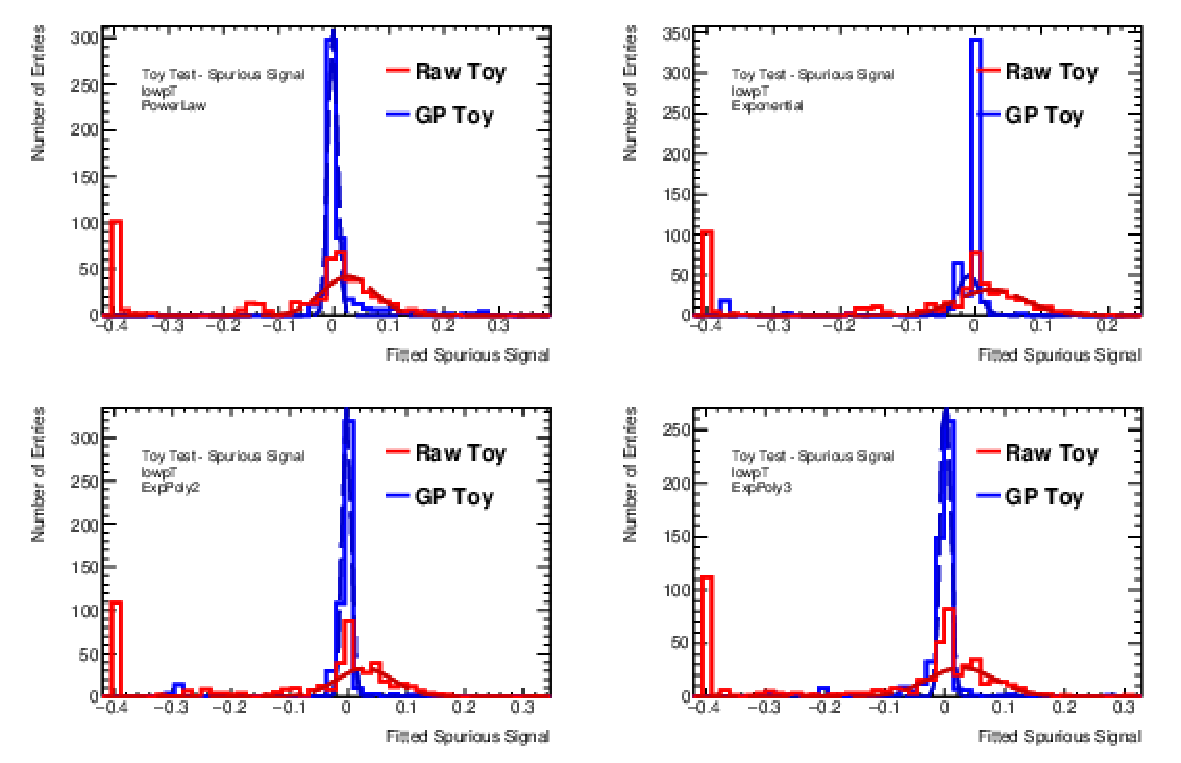
\includegraphics[width=\textwidth]{figures/background/gpr/validation/nominal/ToyTest_FitSigVals_lowpT_10_noSig}   
\caption{The distribution of spurious signal for various functions for both the GPR and raw template, using an expPoly2-derived template. Each toy in this test has 10 events.}
\label{fig:lowpt_10_noSig}
\end{center}
\end{figure}

\begin{figure} 
\begin{center}
  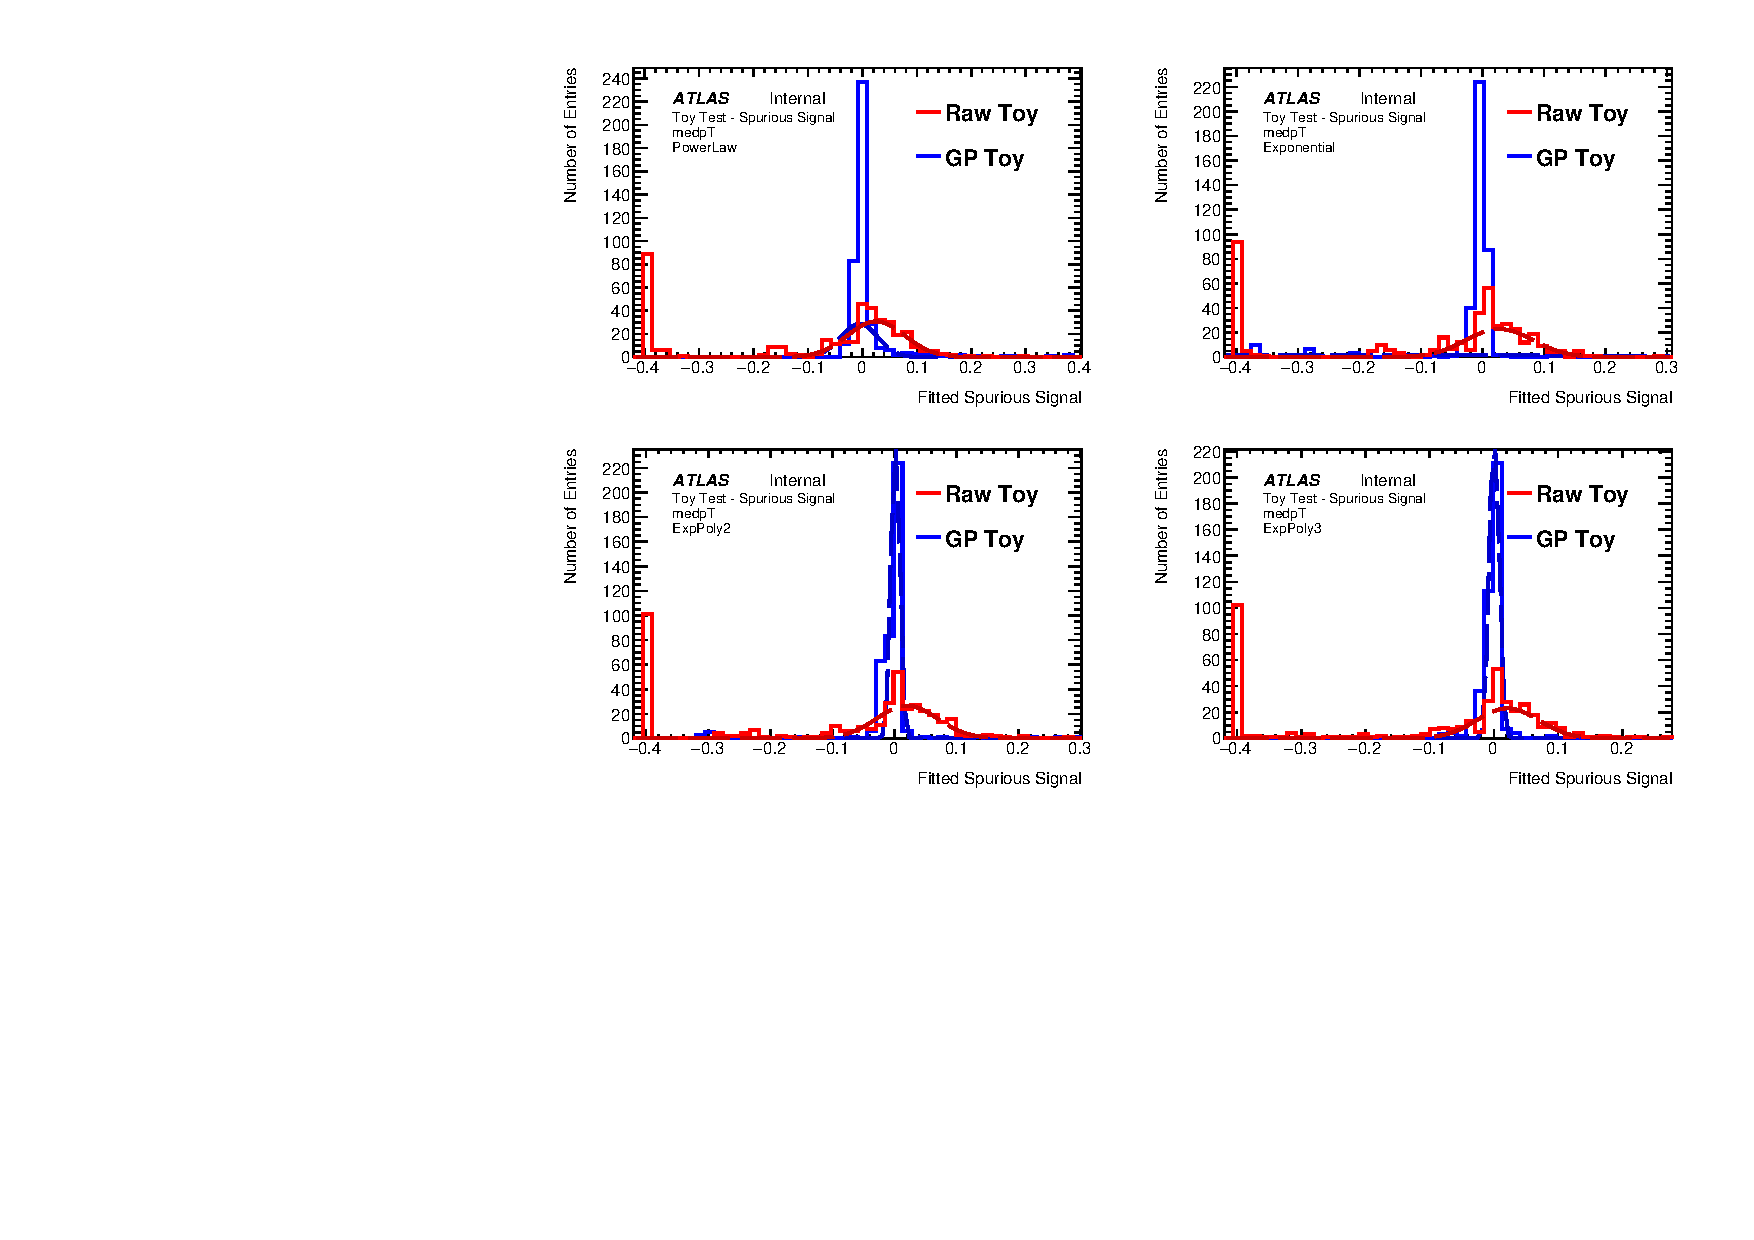
\includegraphics[width=\textwidth]{figures/background/gpr/validation/nominal/ToyTest_FitSigVals_medpT_10_noSig}   
\caption{The distribution of spurious signal for various functions for both the GPR and raw template, using an expPoly3-derived template. Each toy in this test has 10 events.}
\label{fig:medpt_10_noSig}
\end{center}
\end{figure}

\begin{figure} 
\begin{center}
  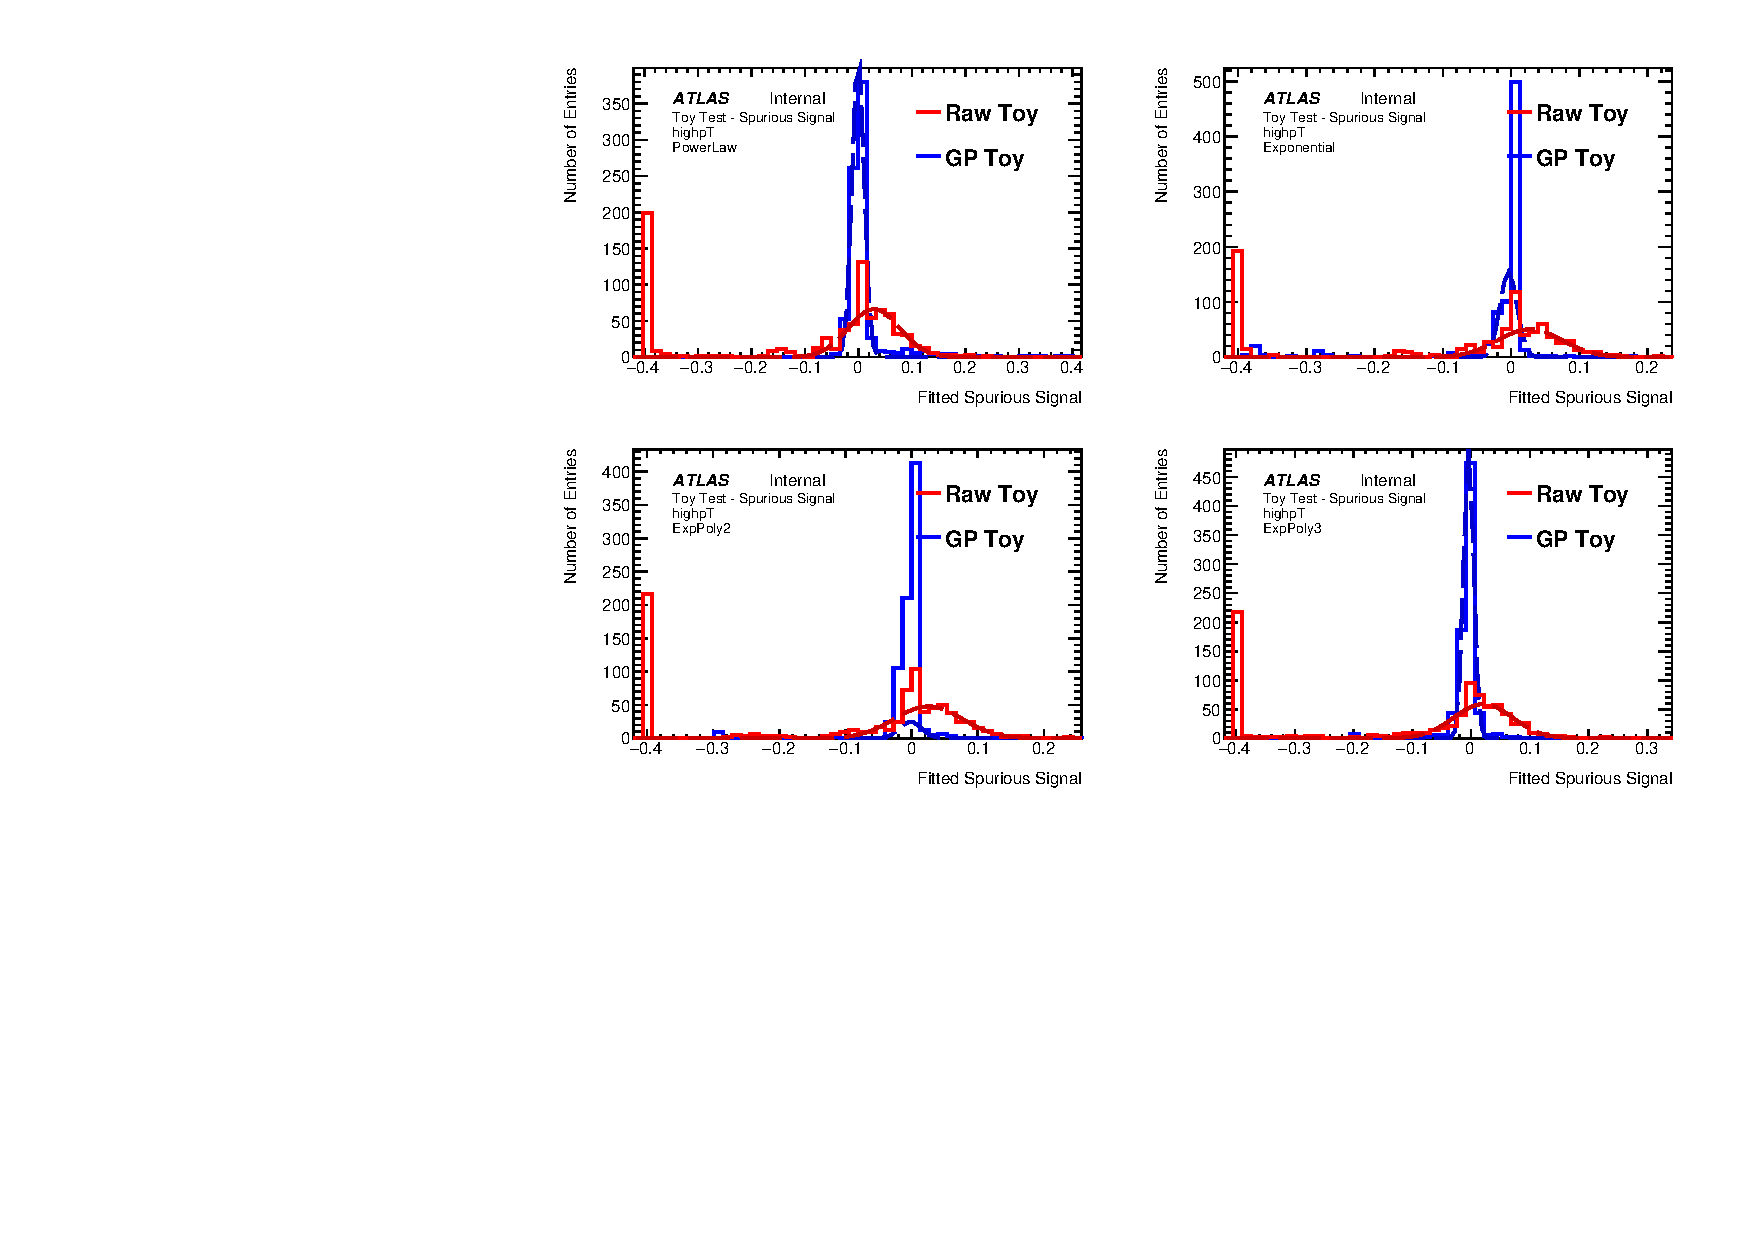
\includegraphics[width=\textwidth]{figures/background/gpr/validation/nominal/ToyTest_FitSigVals_highpT_10_noSig}   
\caption{The distribution of spurious signal for various functions for both the GPR and raw template, using a different expPoly3-derived template. Each toy in this test has 10 events.}
\label{fig:highpt_10_noSig}
\end{center}
\end{figure}

\begin{figure} 
\begin{center}
  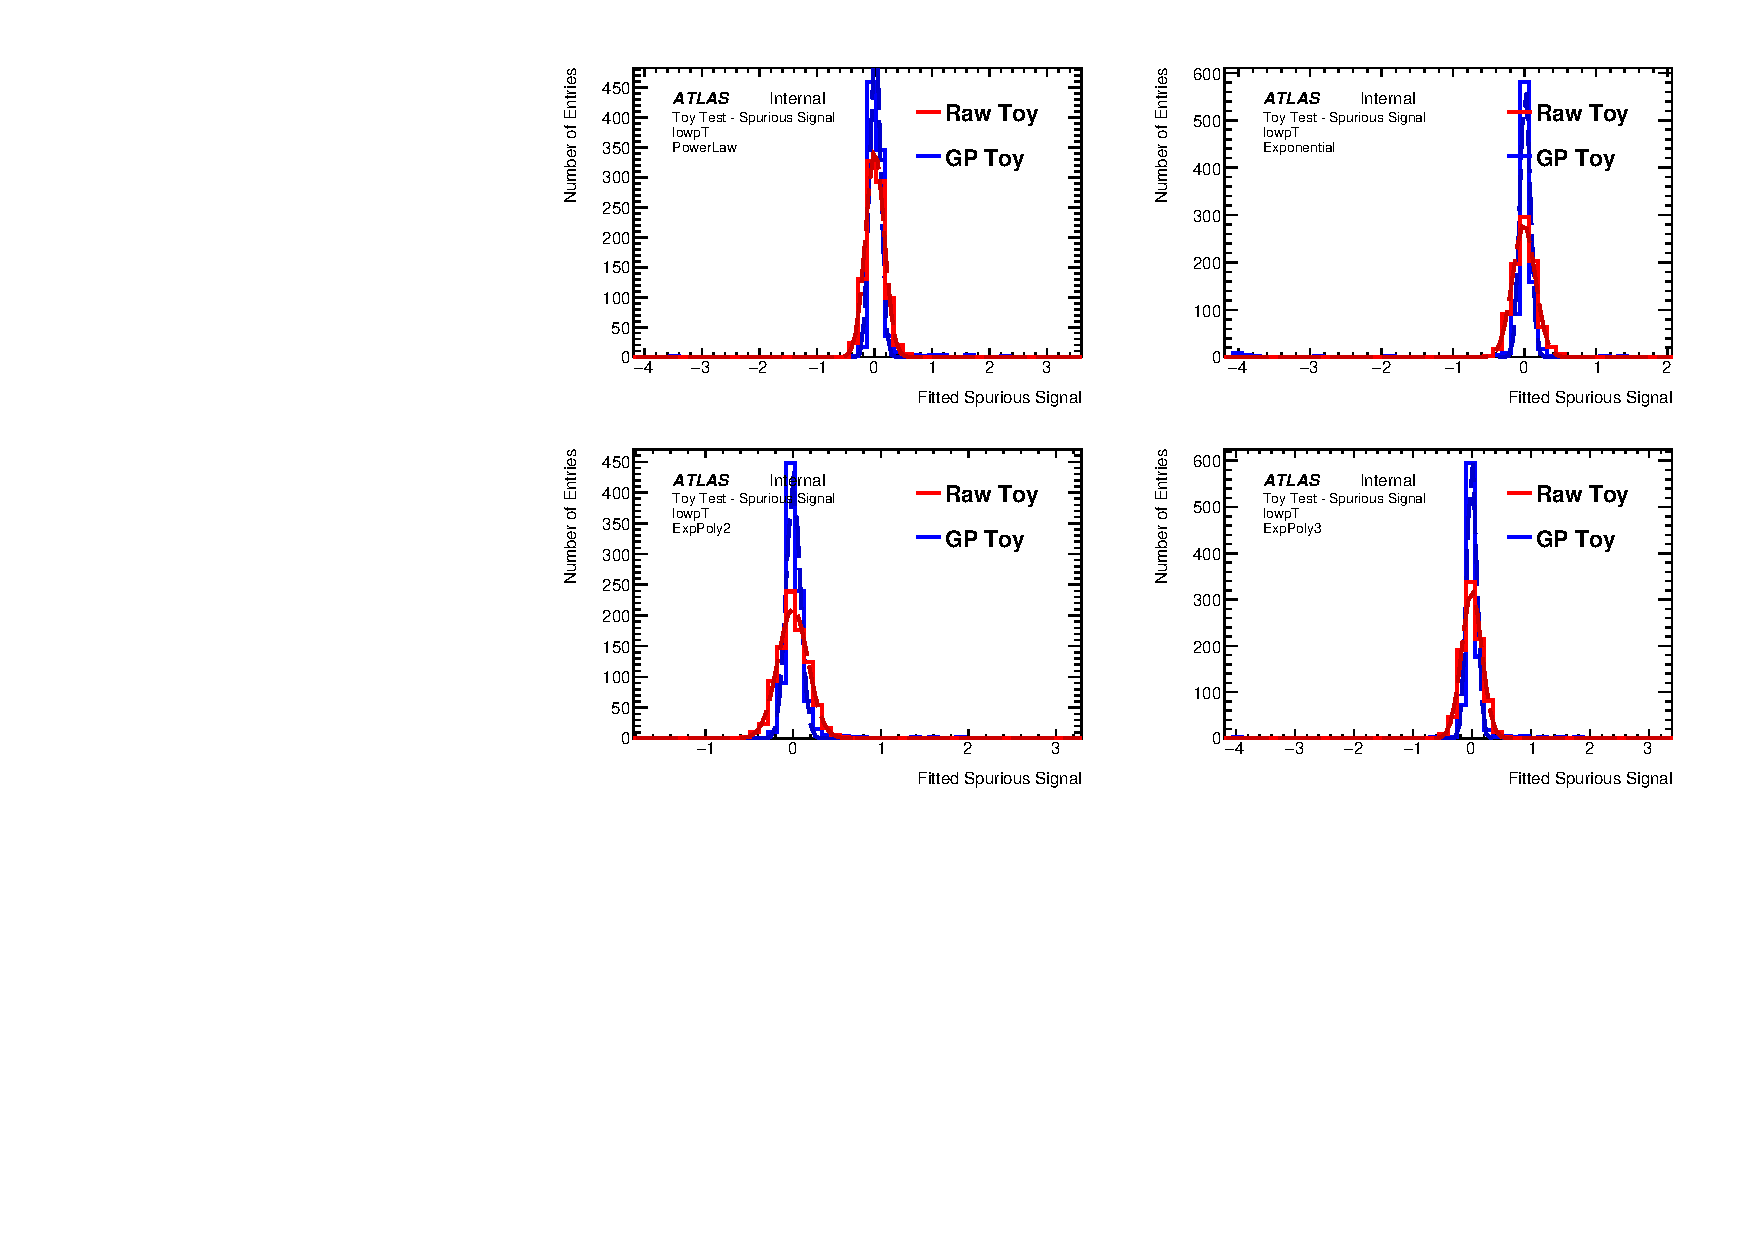
\includegraphics[width=\textwidth]{figures/background/gpr/validation/nominal/ToyTest_FitSigVals_lowpT_100_noSig}   
\caption{The distribution of spurious signal for various functions for both the GPR and raw template, using an expPoly2-derived template. Each toy in this test has 100 events.}
\label{fig:lowpt_100_noSig}
\end{center}
\end{figure}

\begin{figure} 
\begin{center}
  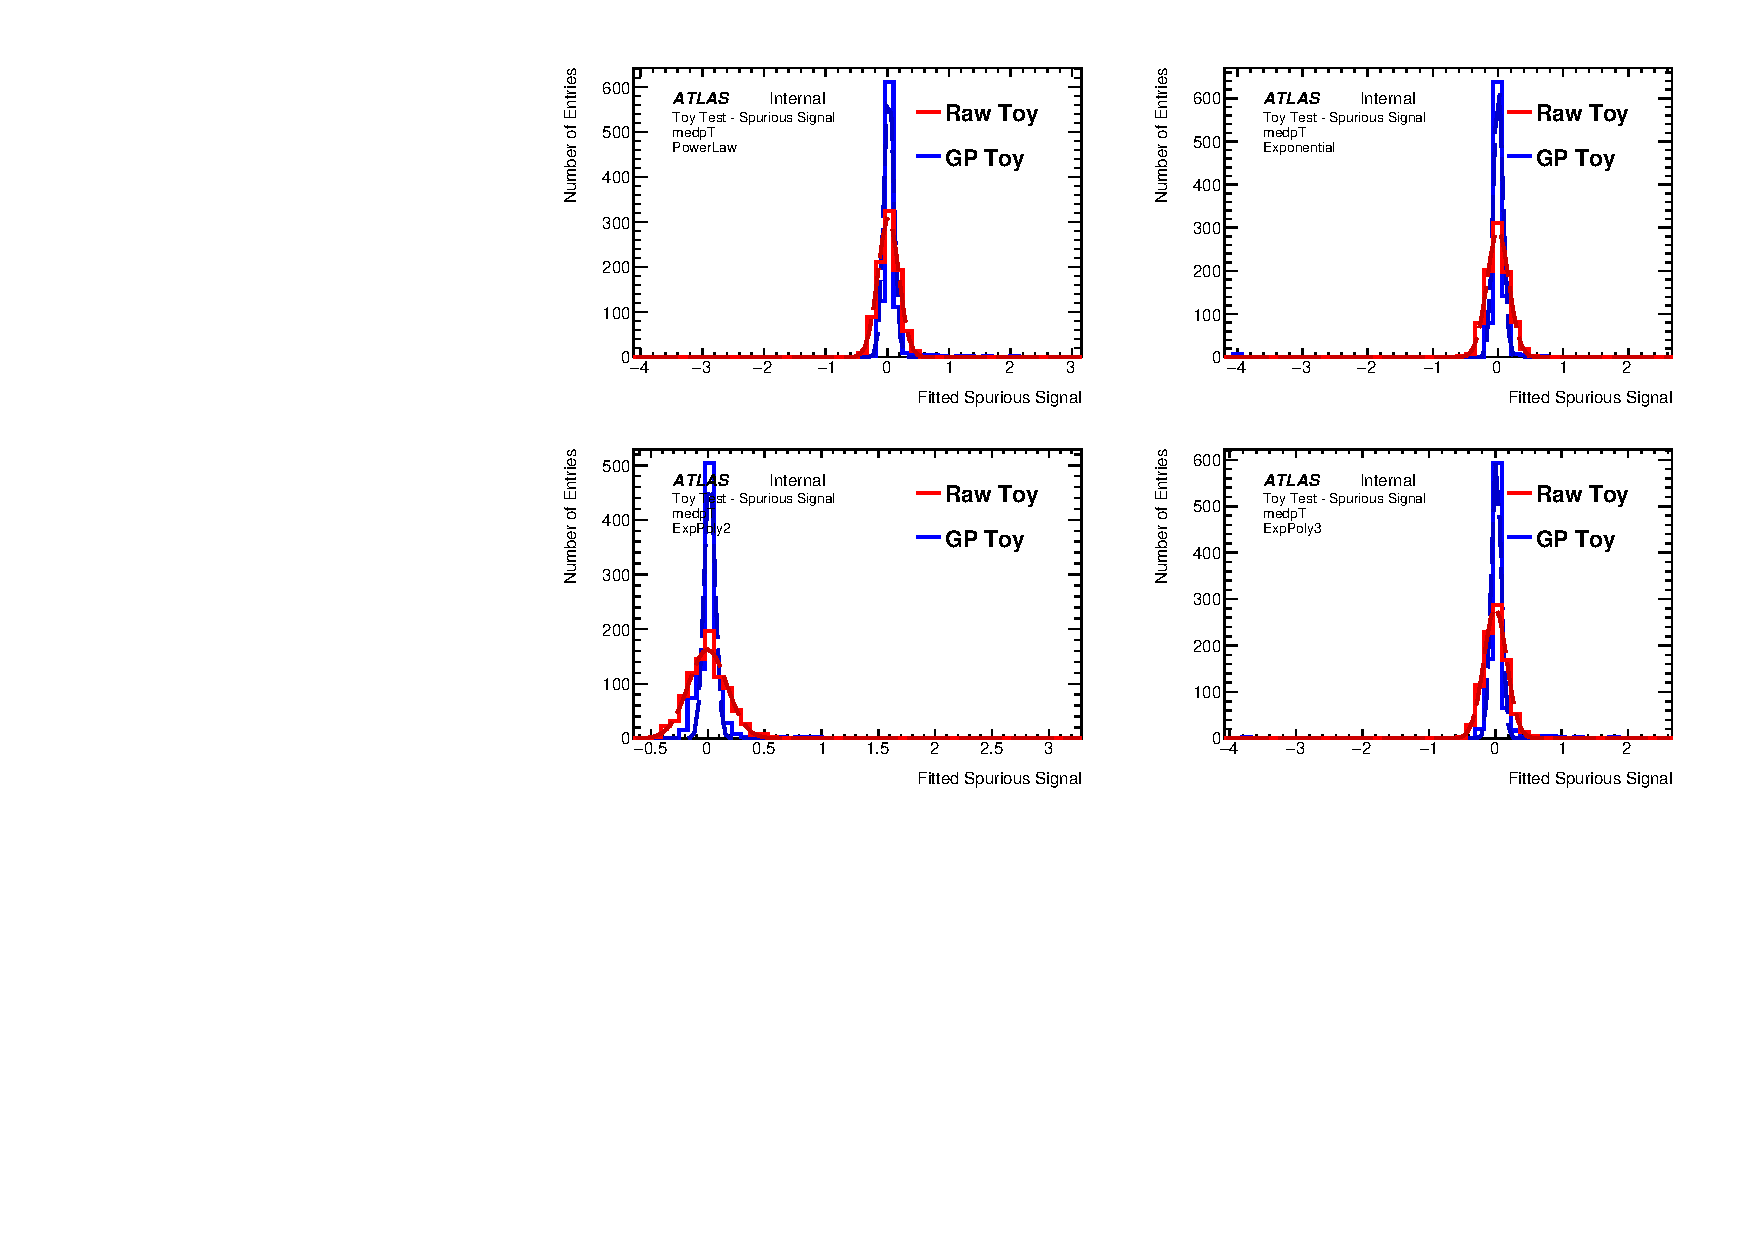
\includegraphics[width=\textwidth]{figures/background/gpr/validation/nominal/ToyTest_FitSigVals_medpT_100_noSig}   
\caption{The distribution of spurious signal for various functions for both the GPR and raw template, using an expPoly3-derived template. Each toy in this test has 100 events.}
\label{fig:medpt_100_noSig}
\end{center}
\end{figure}

\begin{figure} 
\begin{center}
  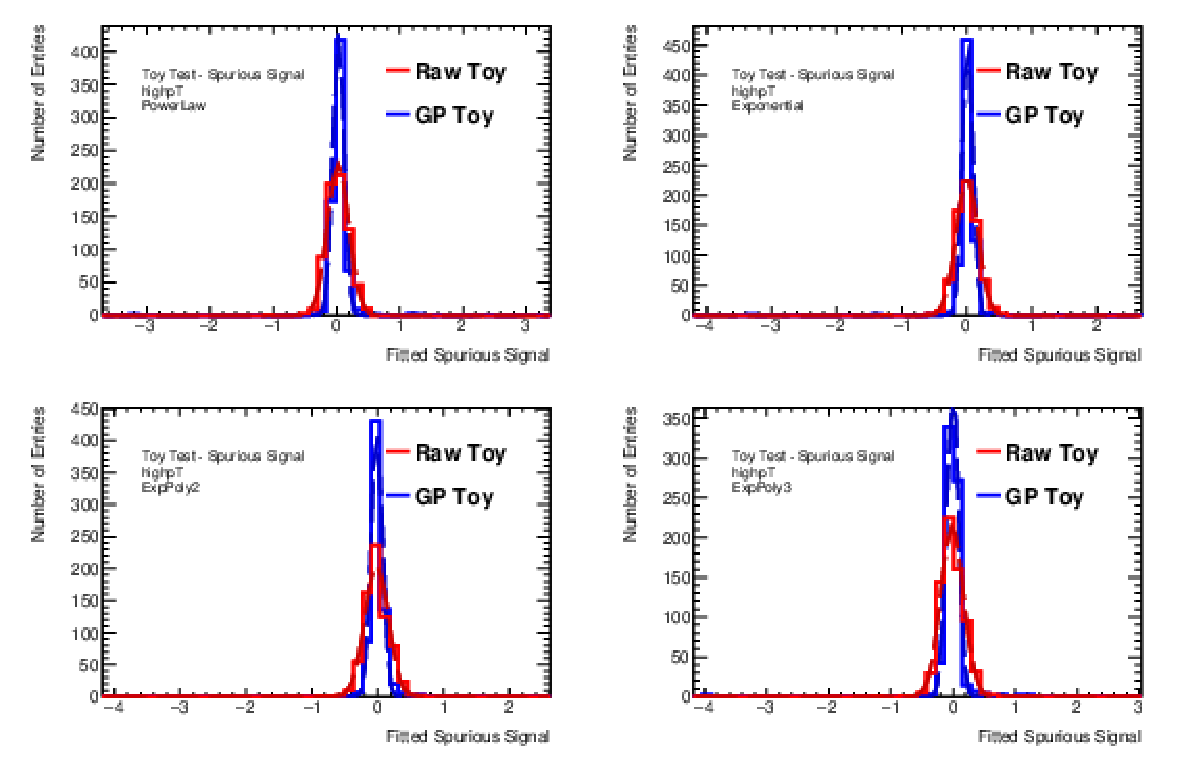
\includegraphics[width=\textwidth]{figures/background/gpr/validation/nominal/ToyTest_FitSigVals_highpT_100_noSig}   
\caption{The distribution of spurious signal for various functions for both the GPR and raw template, using a different expPoly3-derived template. Each toy in this test has 100 events.}
\label{fig:highpt_100_noSig}
\end{center}
\end{figure}

\begin{figure} 
\begin{center}
  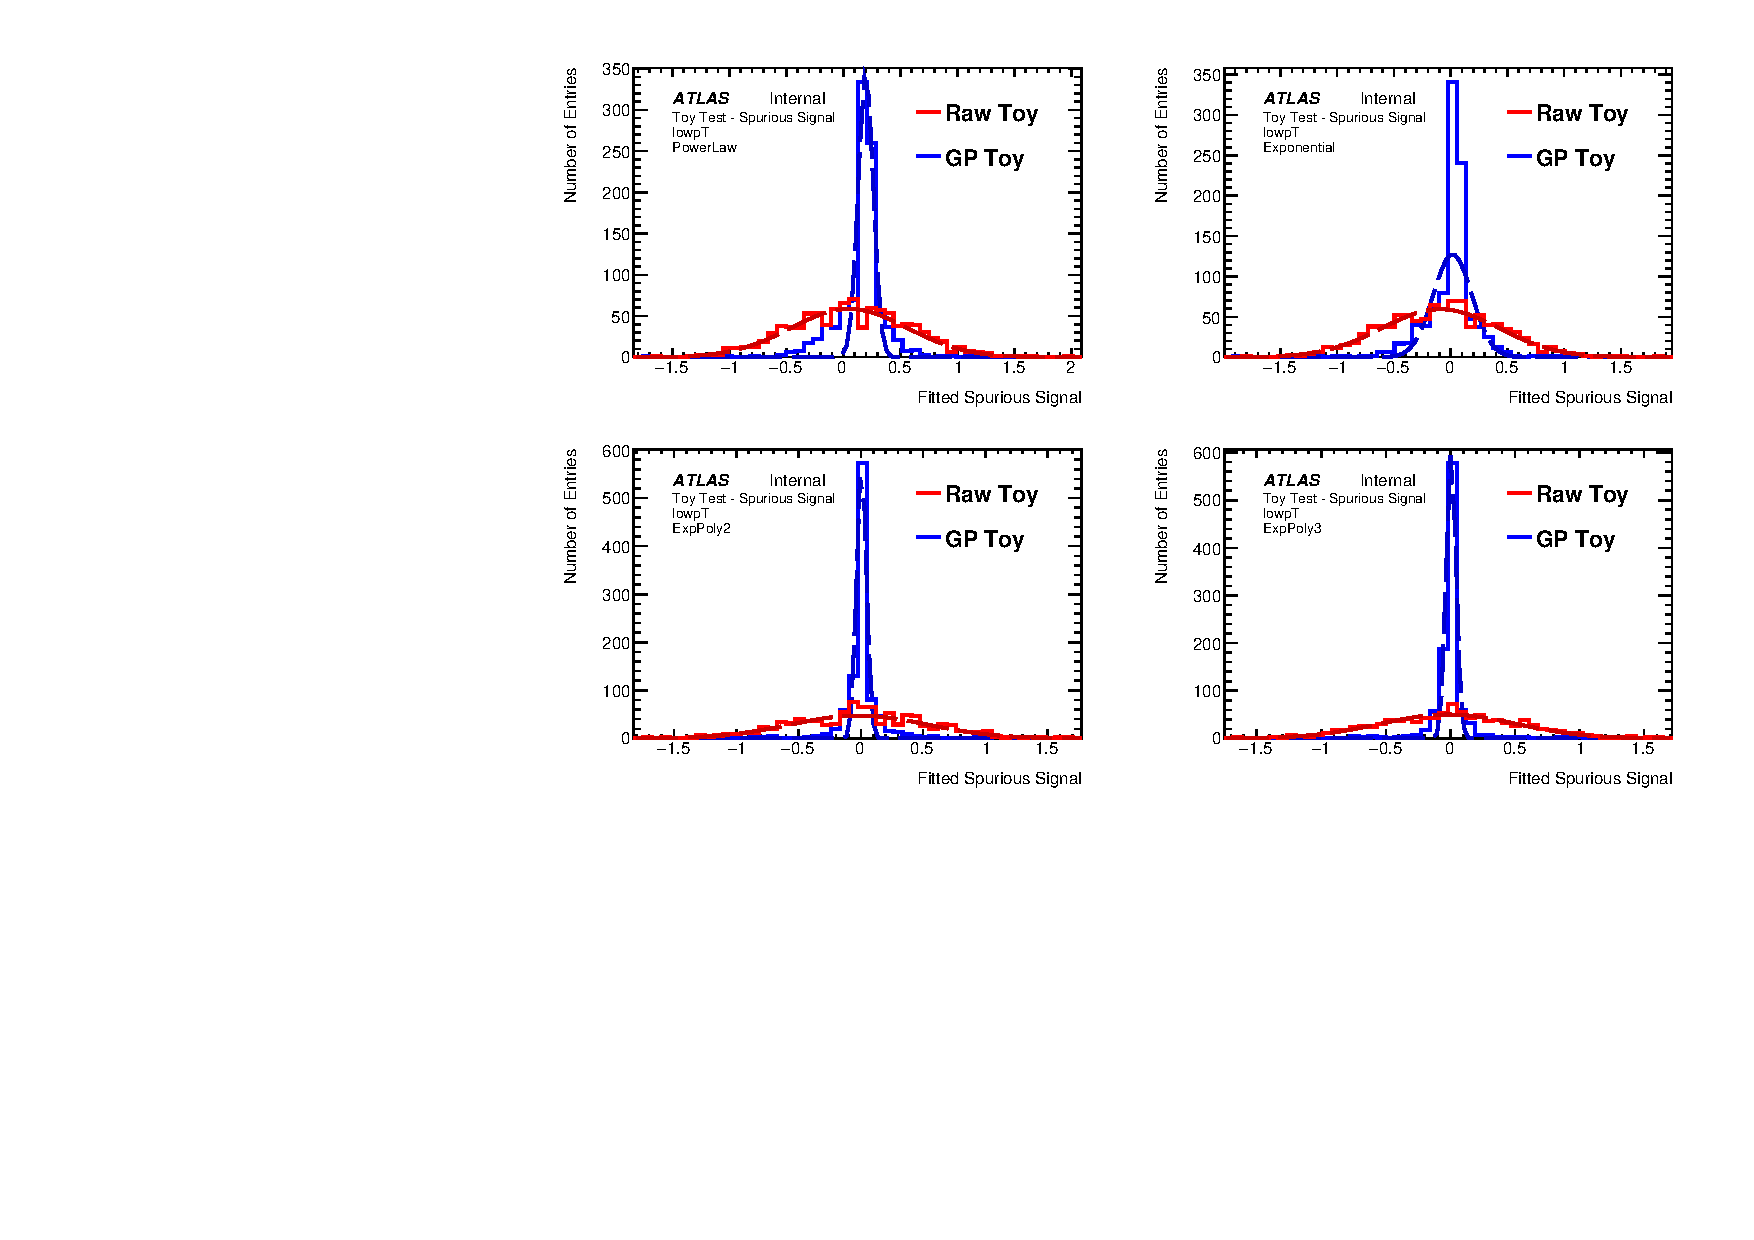
\includegraphics[width=\textwidth]{figures/background/gpr/validation/nominal/ToyTest_FitSigVals_lowpT_1000_noSig}   
\caption{The distribution of spurious signal for various functions for both the GPR and raw template, using an expPoly2-derived template. Each toy in this test has 1000 events.}
\label{fig:lowpt_1000_noSig}
\end{center}
\end{figure}

\begin{figure} 
\begin{center}
  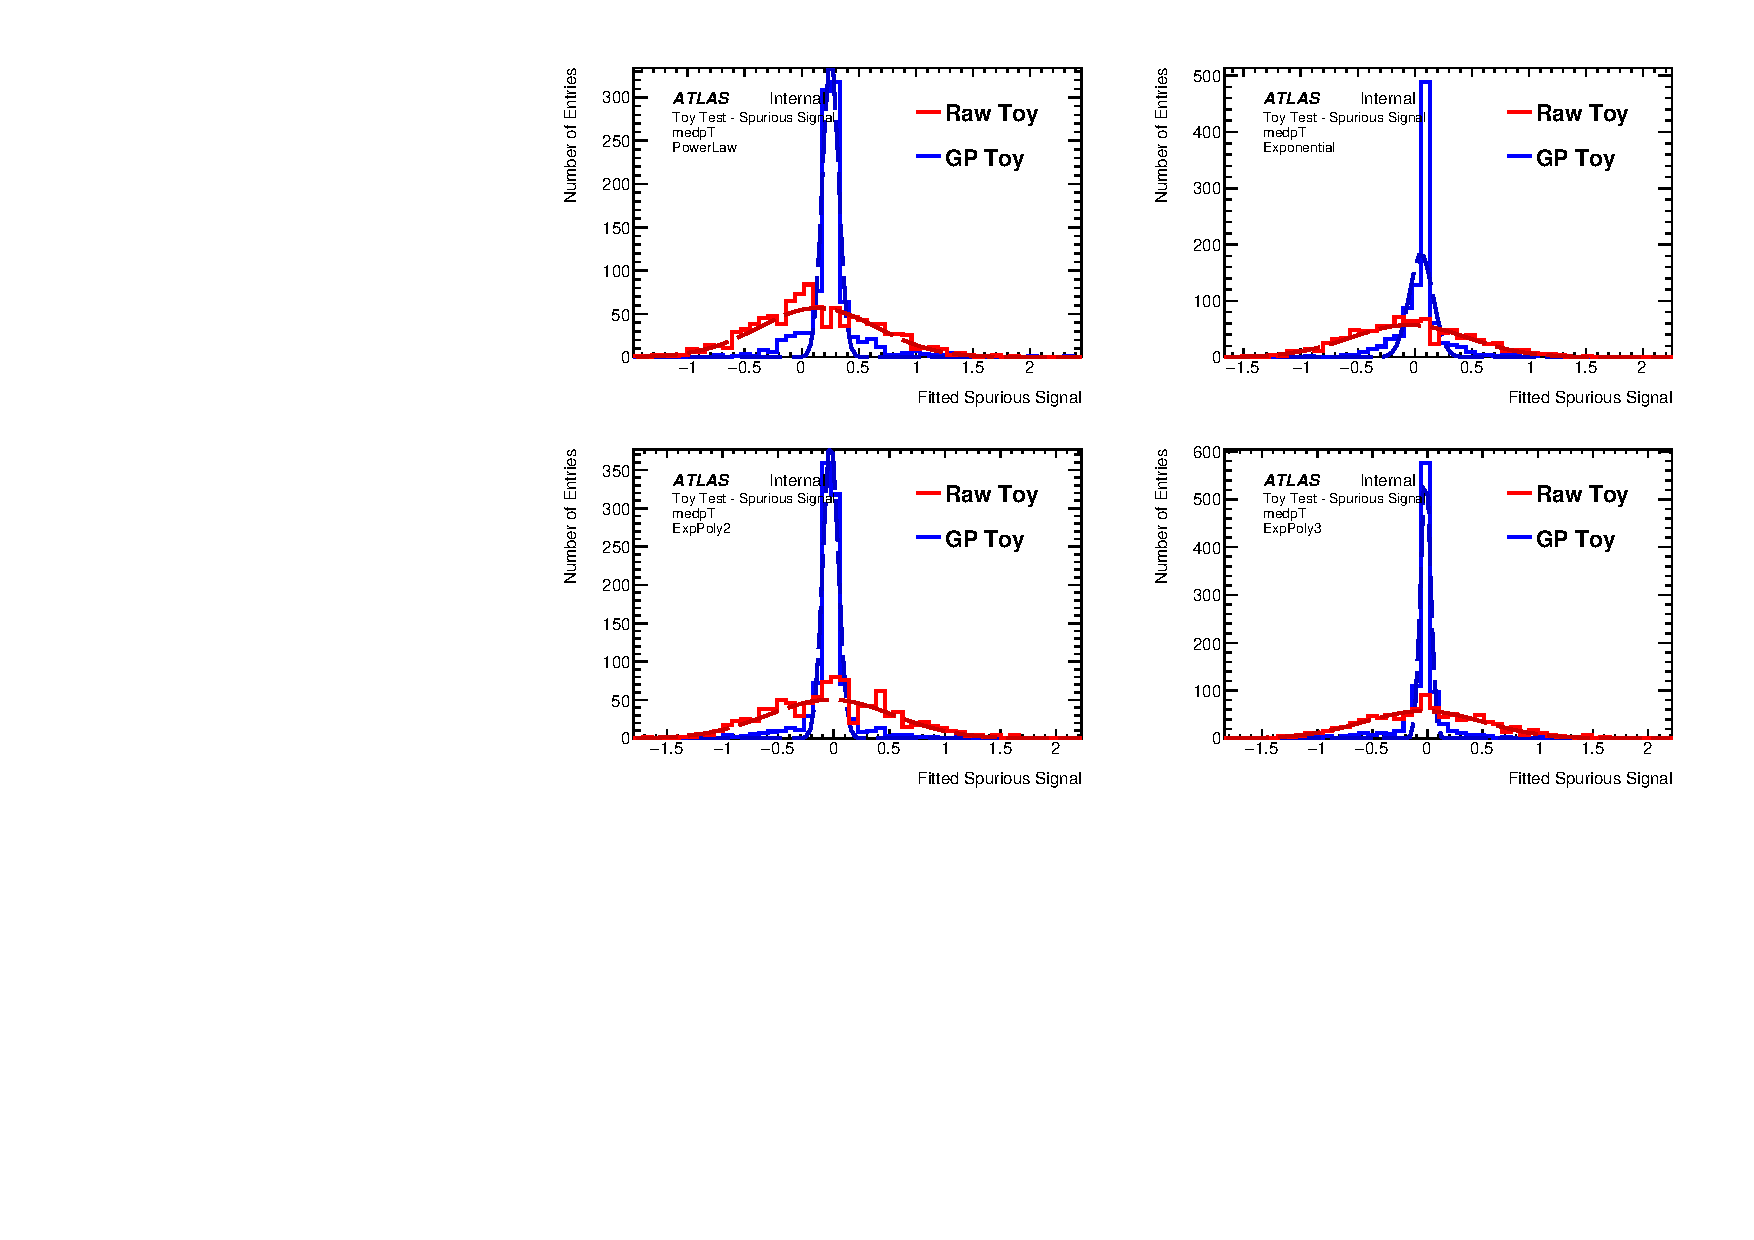
\includegraphics[width=\textwidth]{figures/background/gpr/validation/nominal/ToyTest_FitSigVals_medpT_1000_noSig}   
\caption{The distribution of spurious signal for various functions for both the GPR and raw template, using an expPoly3-derived template. Each toy in this test has 1000 events.}
\label{fig:medpt_1000_noSig}
\end{center}
\end{figure}

\begin{figure} 
\begin{center}
  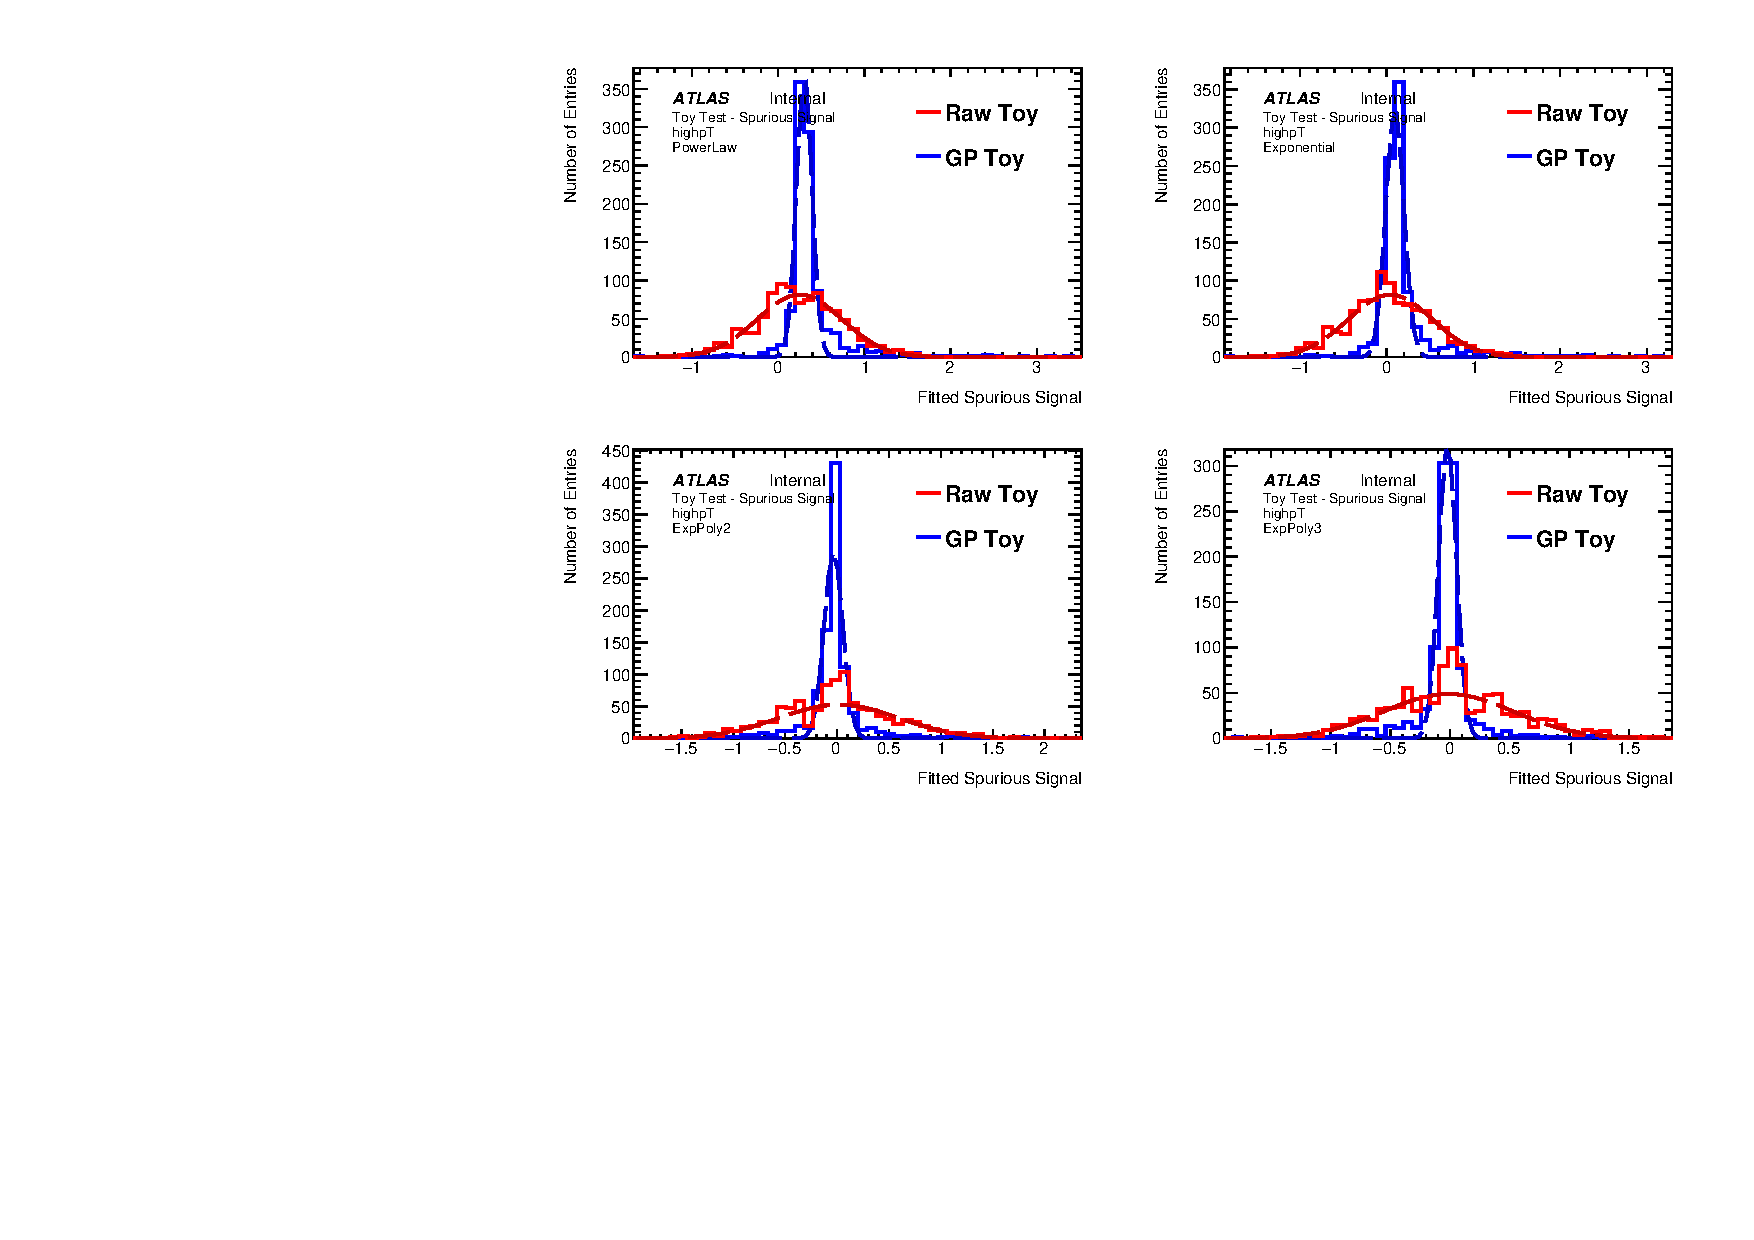
\includegraphics[width=\textwidth]{figures/background/gpr/validation/nominal/ToyTest_FitSigVals_highpT_1000_noSig}   
\caption{The distribution of spurious signal for various functions for both the GPR and raw template, using a different expPoly3-derived template. Each toy in this test has 1000 events.}
\label{fig:highpt_1000_noSig}
\end{center}
\end{figure}

\begin{figure} 
\begin{center}
  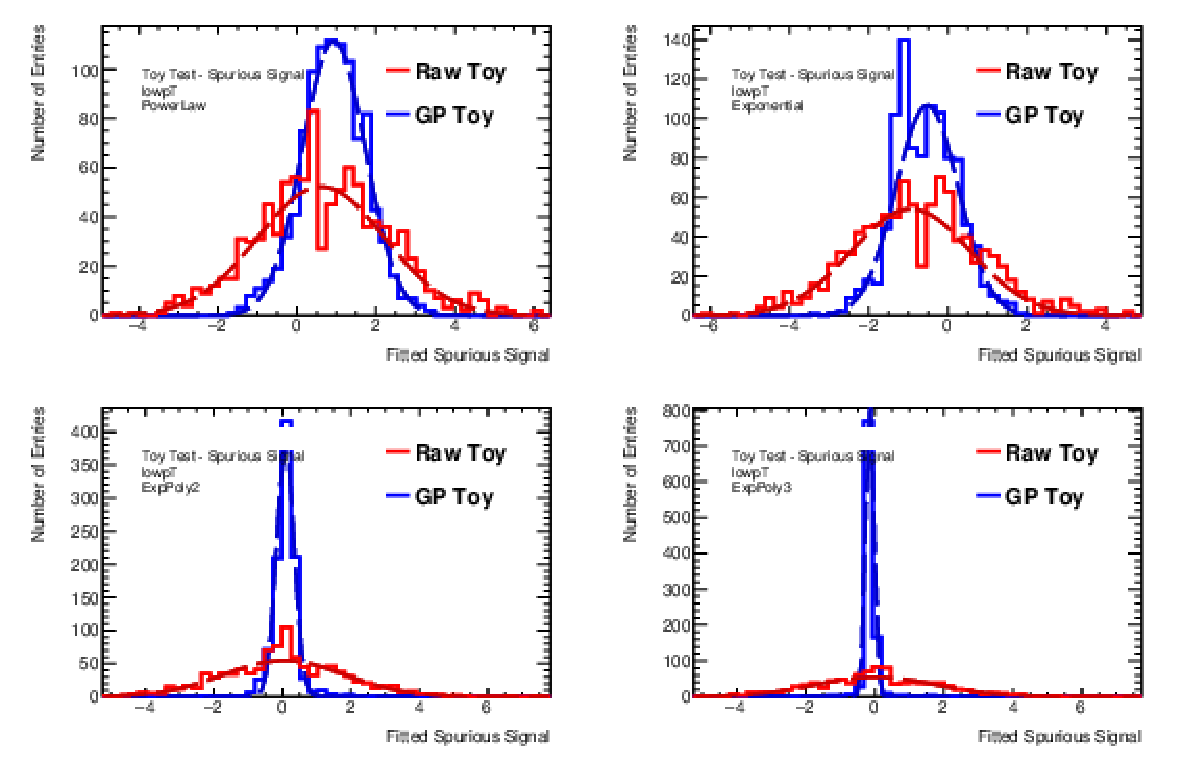
\includegraphics[width=\textwidth]{figures/background/gpr/validation/nominal/ToyTest_FitSigVals_lowpT_10k_noSig}   
\caption{The distribution of spurious signal for various functions for both the GPR and raw template, using an expPoly2-derived template. Each toy in this test has 10k events.}
\label{fig:lowpt_10k_noSig}
\end{center}
\end{figure}

\begin{figure} 
\begin{center}
  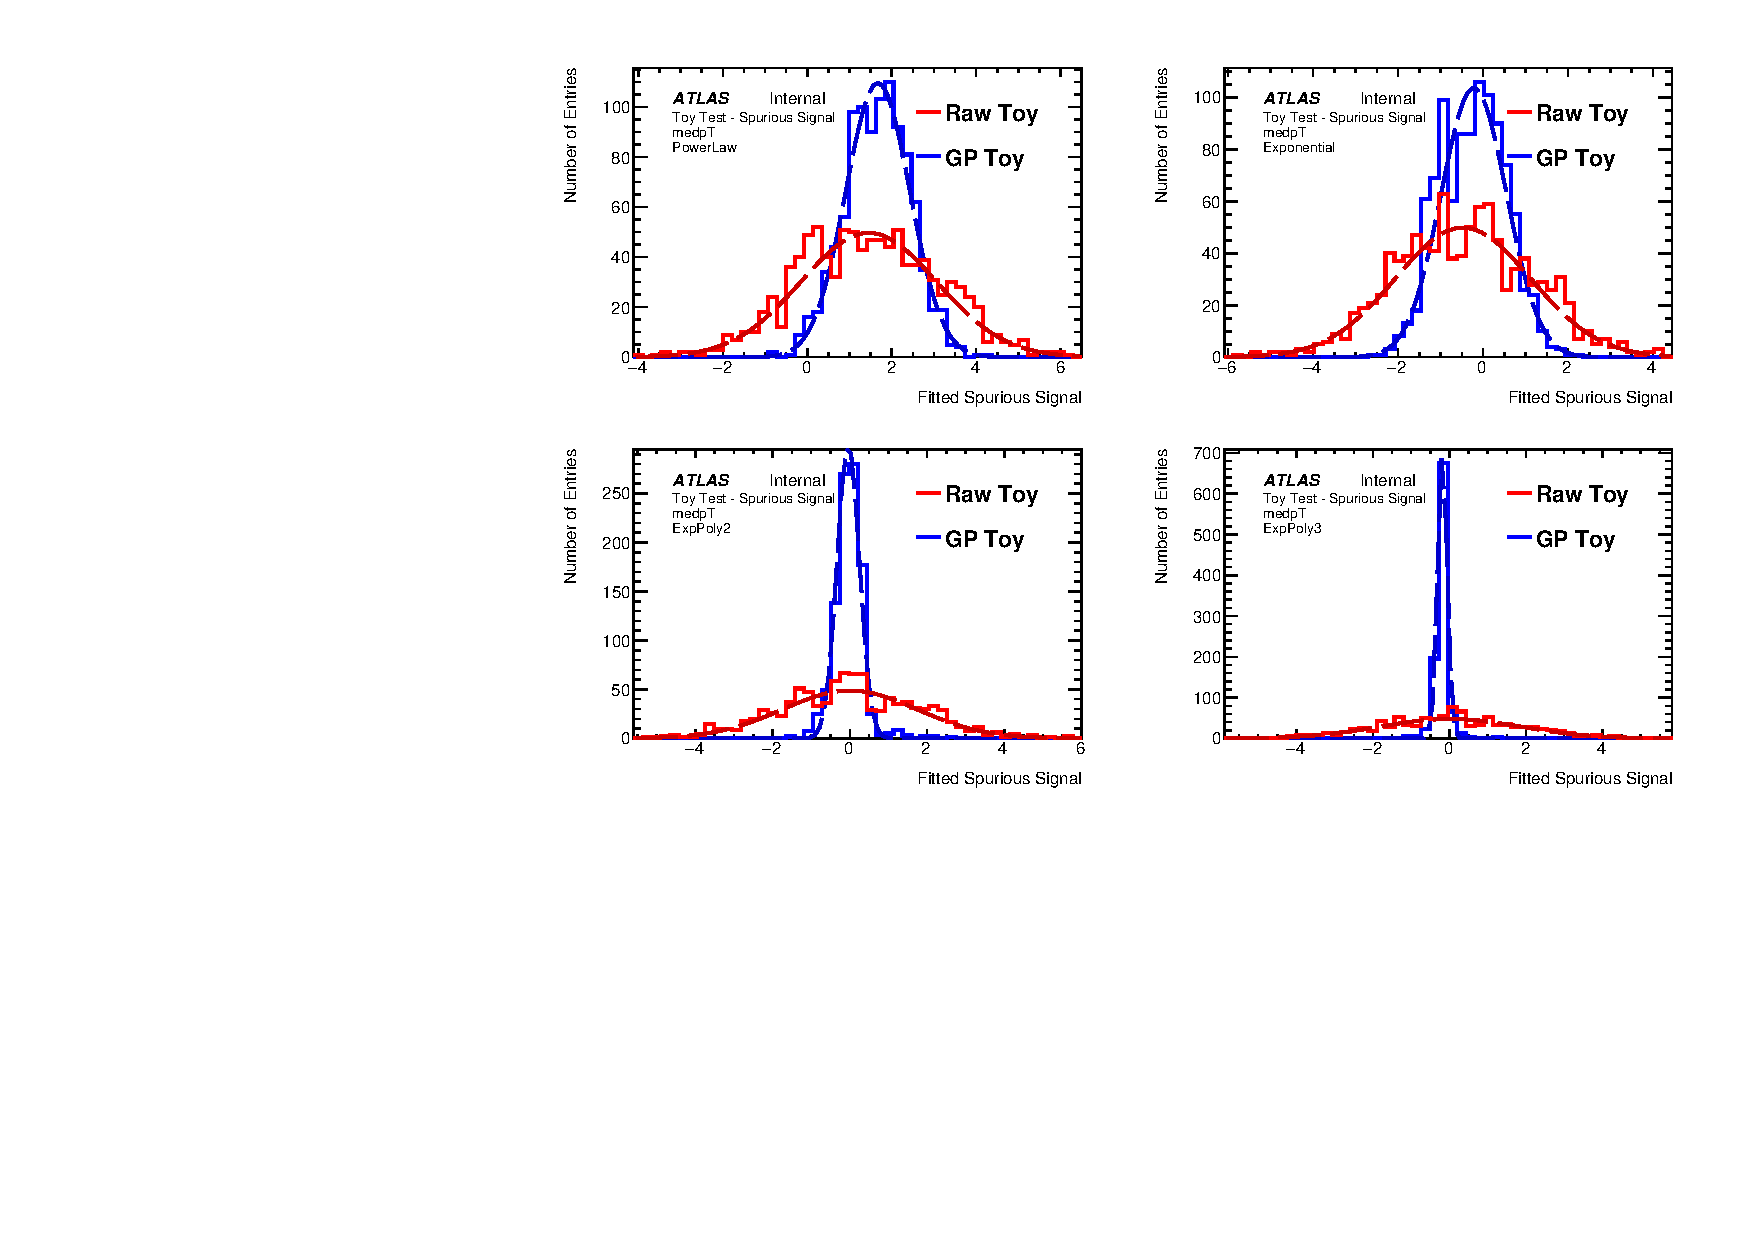
\includegraphics[width=\textwidth]{figures/background/gpr/validation/nominal/ToyTest_FitSigVals_medpT_10k_noSig}   
\caption{The distribution of spurious signal for various functions for both the GPR and raw template, using an expPoly3-derived template. Each toy in this test has 10k events.}
\label{fig:medpt_10k_noSig}
\end{center}
\end{figure}

\begin{figure} 
\begin{center}
  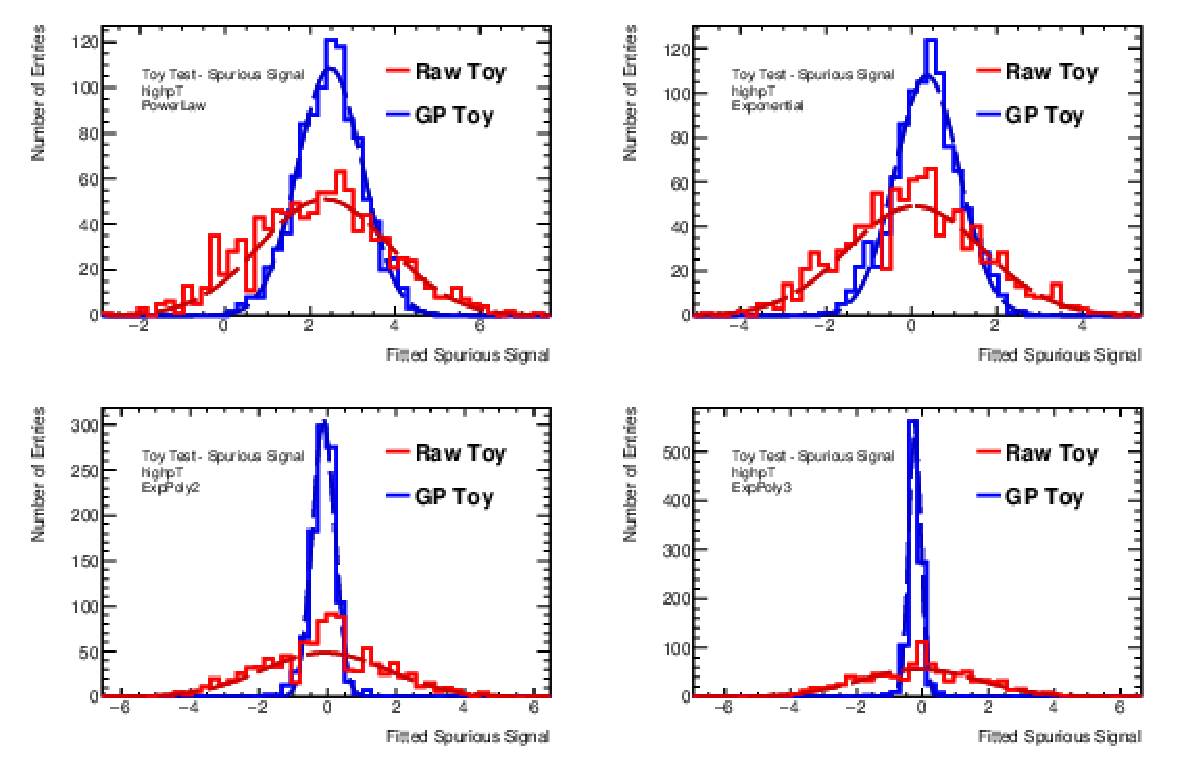
\includegraphics[width=\textwidth]{figures/background/gpr/validation/nominal/ToyTest_FitSigVals_highpT_10k_noSig}   
\caption{The distribution of spurious signal for various functions for both the GPR and raw template, using a different expPoly3-derived template. Each toy in this test has 10k events.}
\label{fig:highpt_10k_noSig}
\end{center}
\end{figure}

\begin{figure} 
\begin{center}
  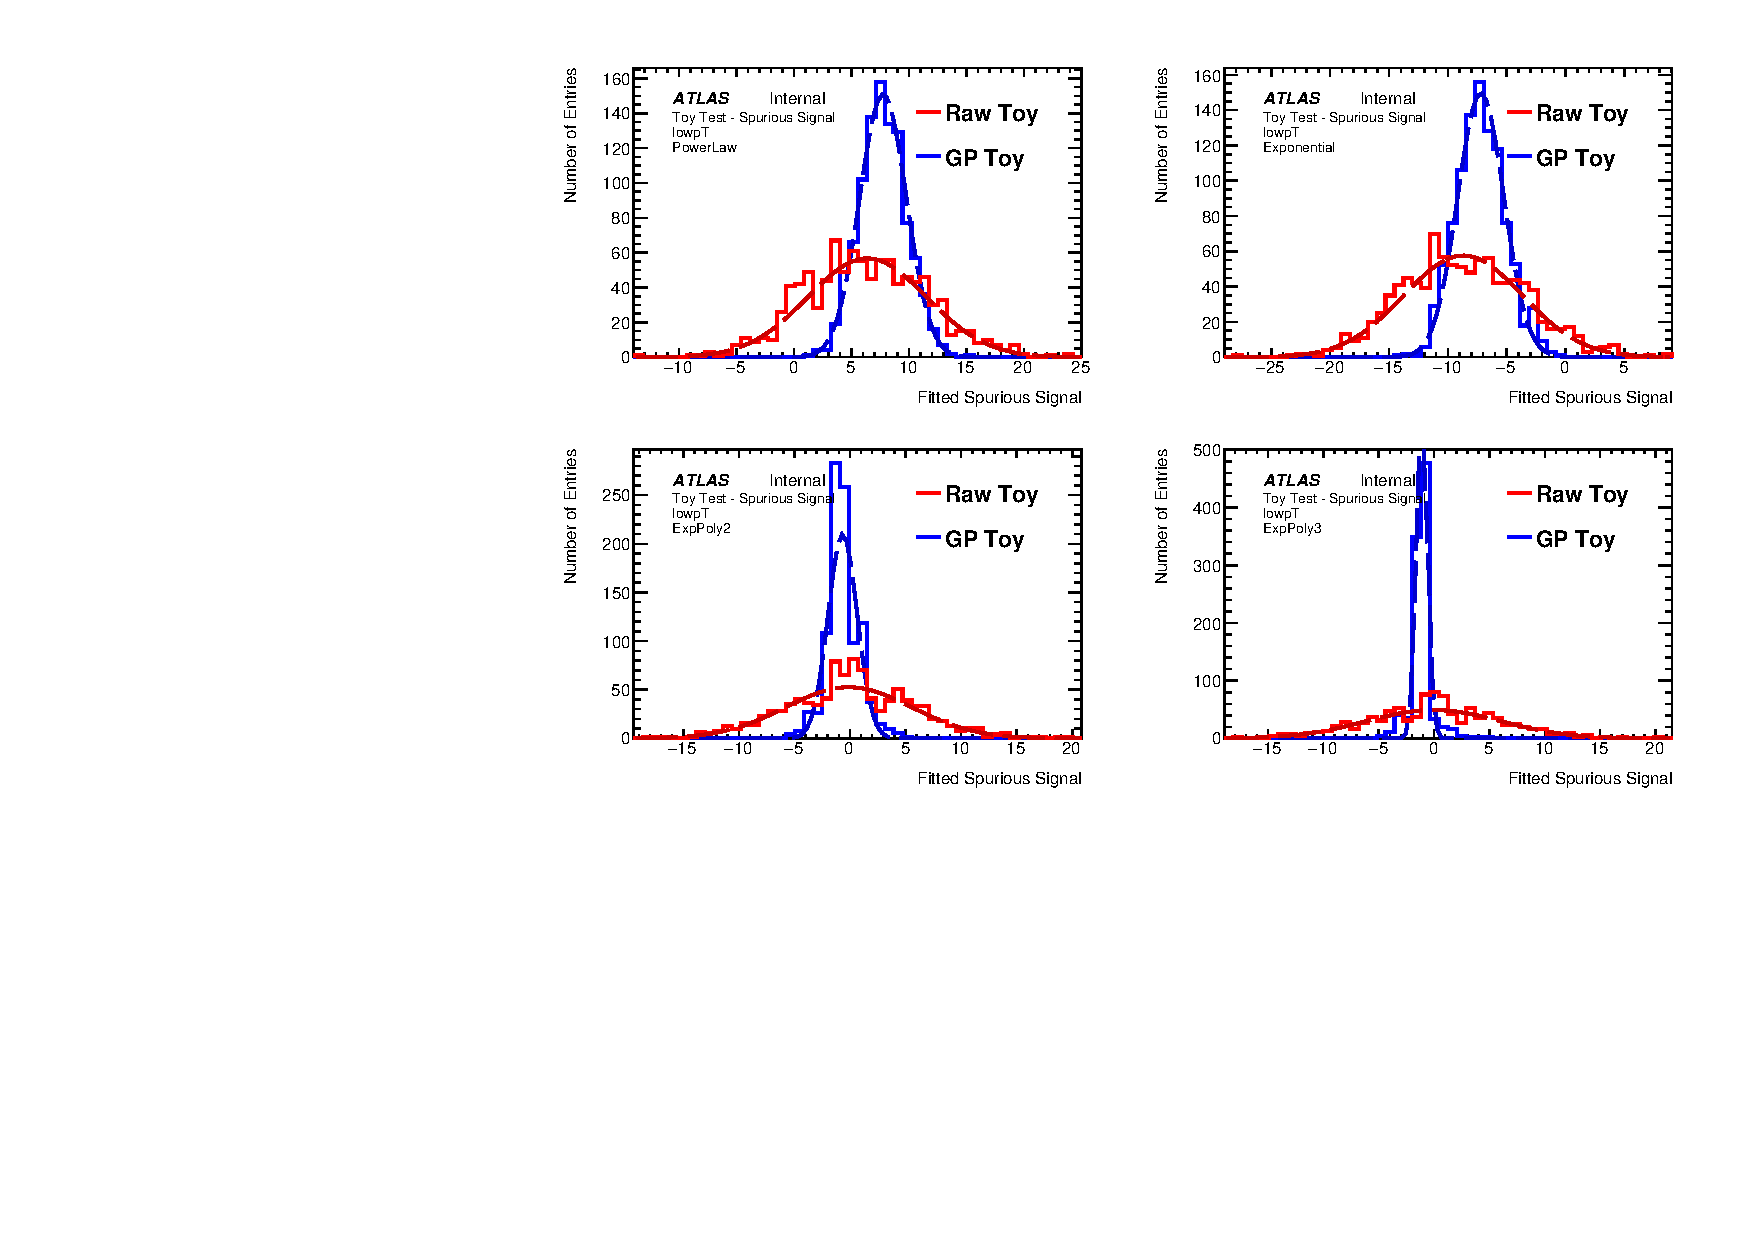
\includegraphics[width=\textwidth]{figures/background/gpr/validation/nominal/ToyTest_FitSigVals_lowpT_100k_noSig}   
\caption{The distribution of spurious signal for various functions for both the GPR and raw template, using an expPoly2-derived template. Each toy in this test has 100k events.}
\label{fig:lowpt_100k_noSig}
\end{center}
\end{figure}

\begin{figure} 
\begin{center}
  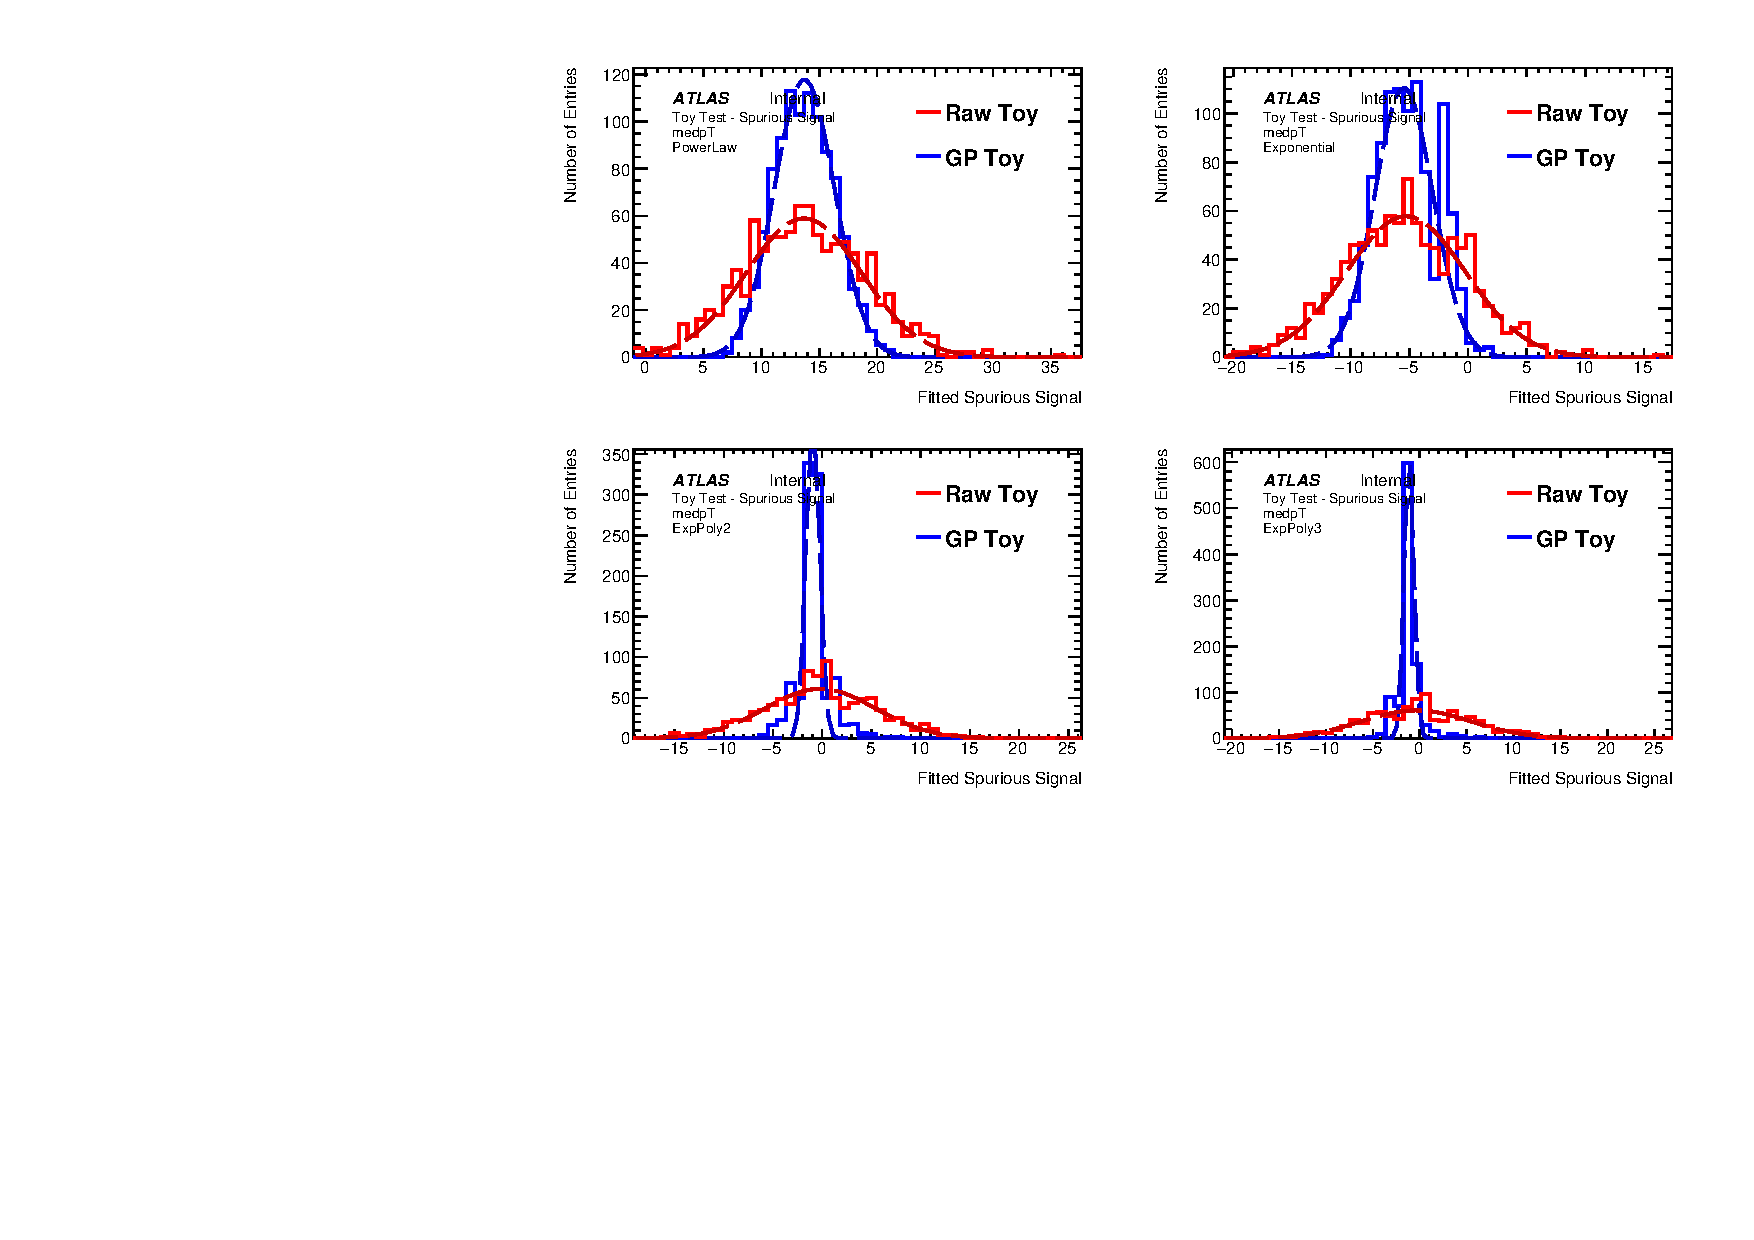
\includegraphics[width=\textwidth]{figures/background/gpr/validation/nominal/ToyTest_FitSigVals_medpT_100k_noSig}   
\caption{The distribution of spurious signal for various functions for both the GPR and raw template, using an expPoly3-derived template. Each toy in this test has 100k events.}
\label{fig:medpt_100k_noSig}
\end{center}
\end{figure}

\begin{figure} 
\begin{center}
  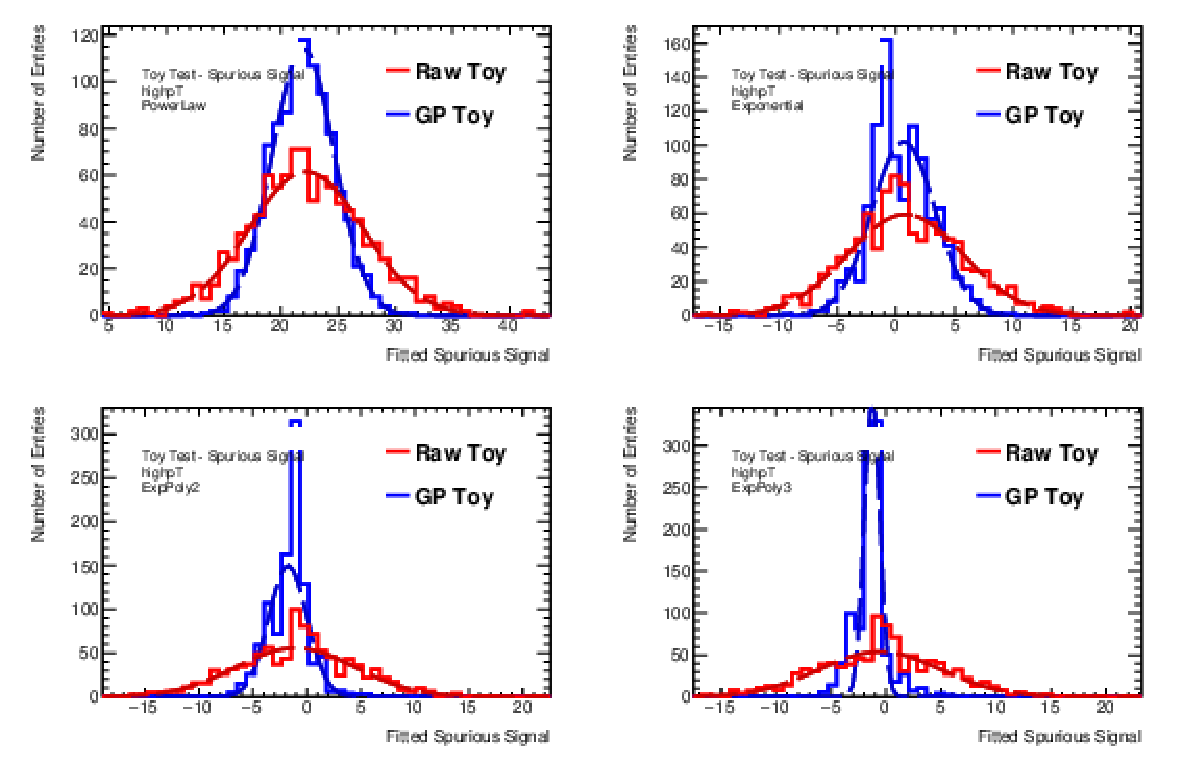
\includegraphics[width=\textwidth]{figures/background/gpr/validation/nominal/ToyTest_FitSigVals_highpT_100k_noSig}   
\caption{The distribution of spurious signal for various functions for both the GPR and raw template, using a different expPoly3-derived template. Each toy in this test has 100k events.}
\label{fig:highpt_100k_noSig}
\end{center}
\end{figure}

\begin{figure} 
\begin{center}
  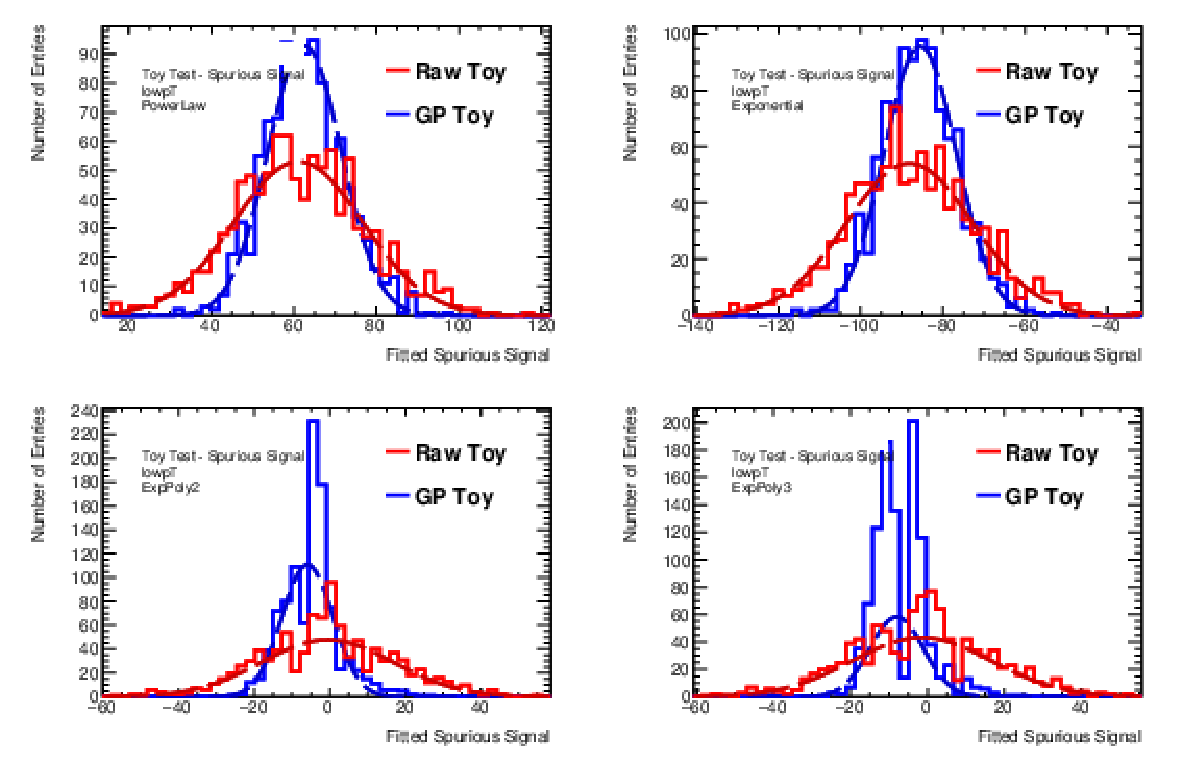
\includegraphics[width=\textwidth]{figures/background/gpr/validation/nominal/ToyTest_FitSigVals_lowpT_1M_noSig}   
\caption{The distribution of spurious signal for various functions for both the GPR and raw template, using an expPoly2-derived template. Each toy in this test has 1,000,000 events.}
\label{fig:lowpt_1M_noSig}
\end{center}
\end{figure}

\begin{figure} 
\begin{center}
  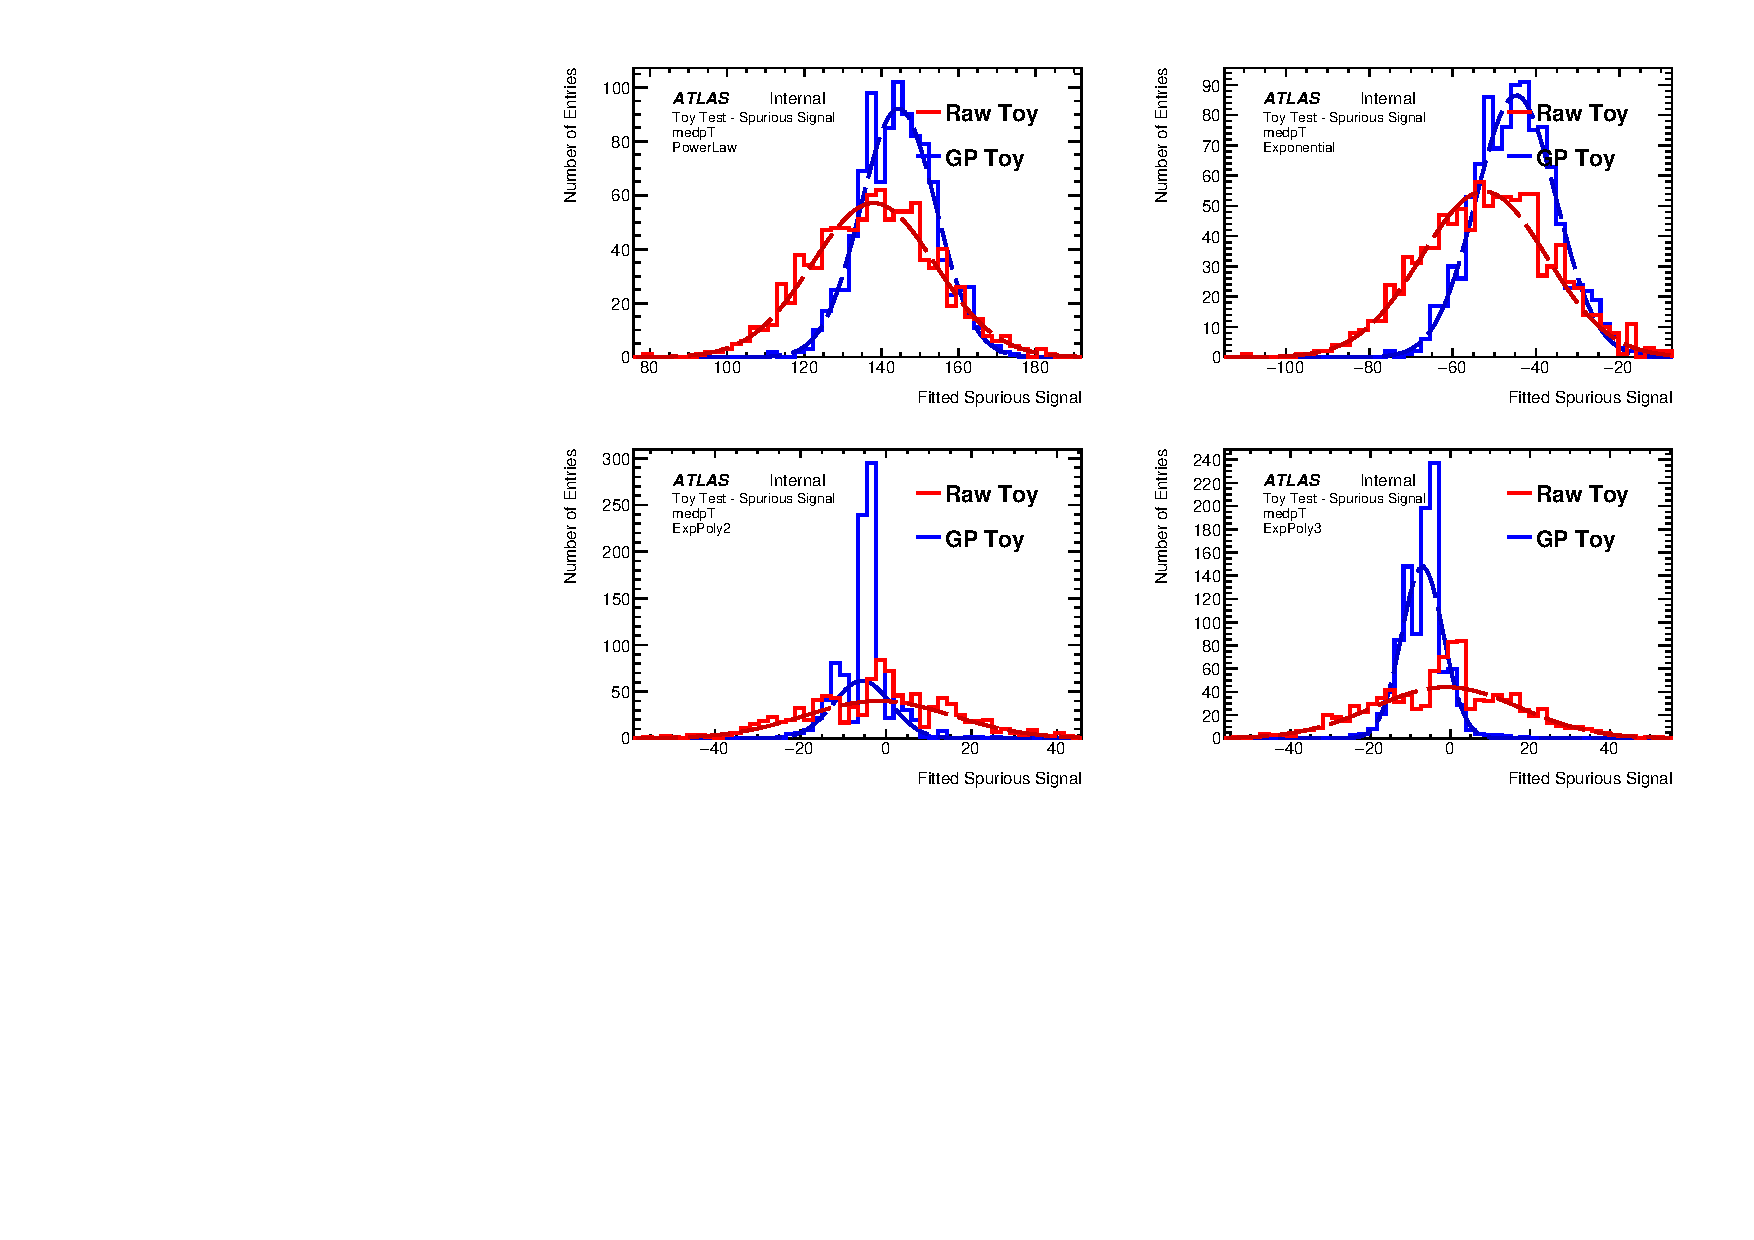
\includegraphics[width=\textwidth]{figures/background/gpr/validation/nominal/ToyTest_FitSigVals_medpT_1M_noSig}   
\caption{The distribution of spurious signal for various functions for both the GPR and raw template, using an expPoly3-derived template. Each toy in this test has 1,000,000 events.}
\label{fig:medpt_1M_noSig}
\end{center}
\end{figure}

\begin{figure} 
\begin{center}
  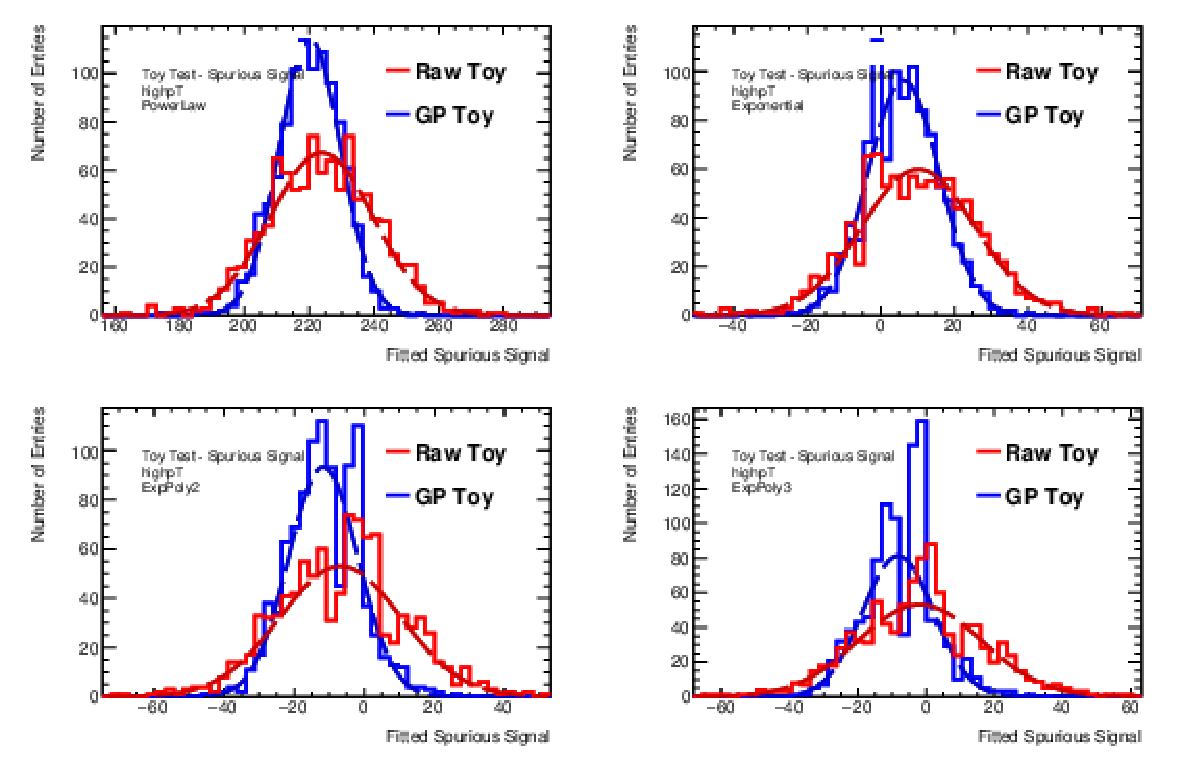
\includegraphics[width=\textwidth]{figures/background/gpr/validation/nominal/ToyTest_FitSigVals_highpT_1M_noSig}   
\caption{The distribution of spurious signal for various functions for both the GPR and raw template, using a different expPoly3-derived template. Each toy in this test has 1,000,000 events.}
\label{fig:highpt_1M_noSig}
\end{center}
\end{figure}

\begin{figure} 
\begin{center}
  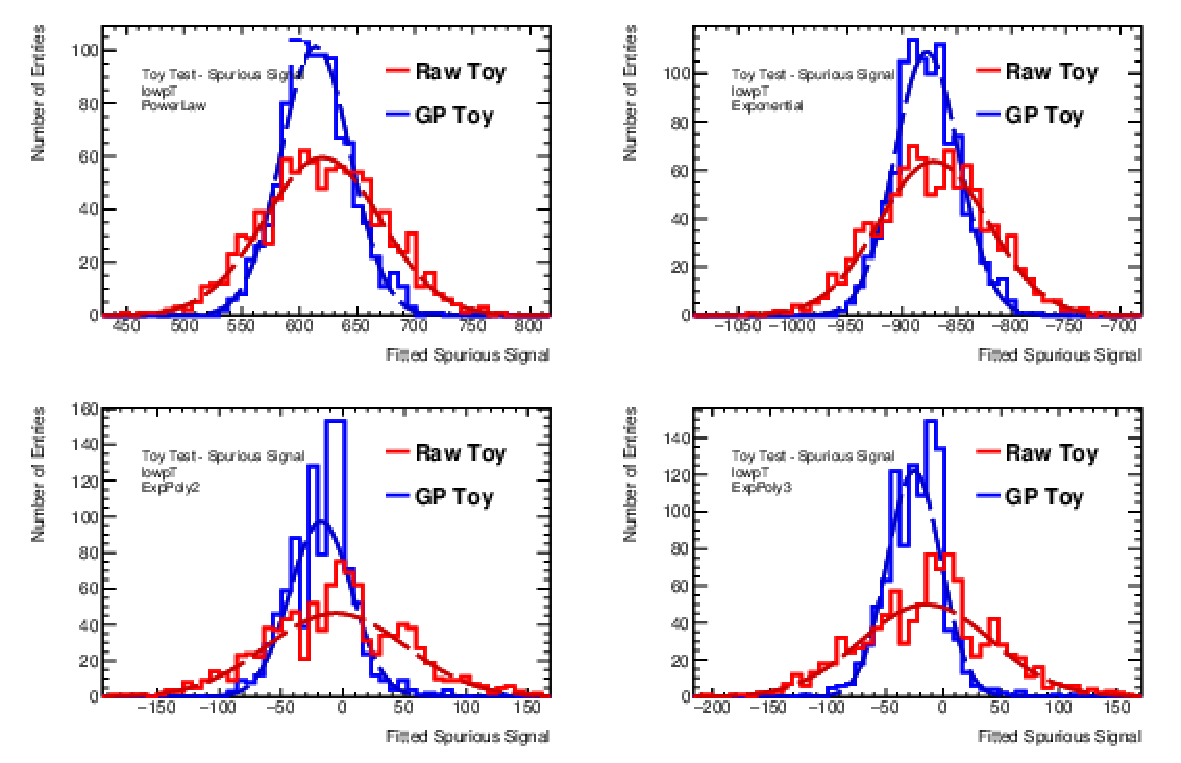
\includegraphics[width=\textwidth]{figures/background/gpr/validation/nominal/ToyTest_FitSigVals_lowpT_10M_noSig}   
\caption{The distribution of spurious signal for various functions for both the GPR and raw template, using an expPoly2-derived template. Each toy in this test has 10,000,000 events.}
\label{fig:lowpt_10M_noSig}
\end{center}
\end{figure}

\begin{figure} 
\begin{center}
  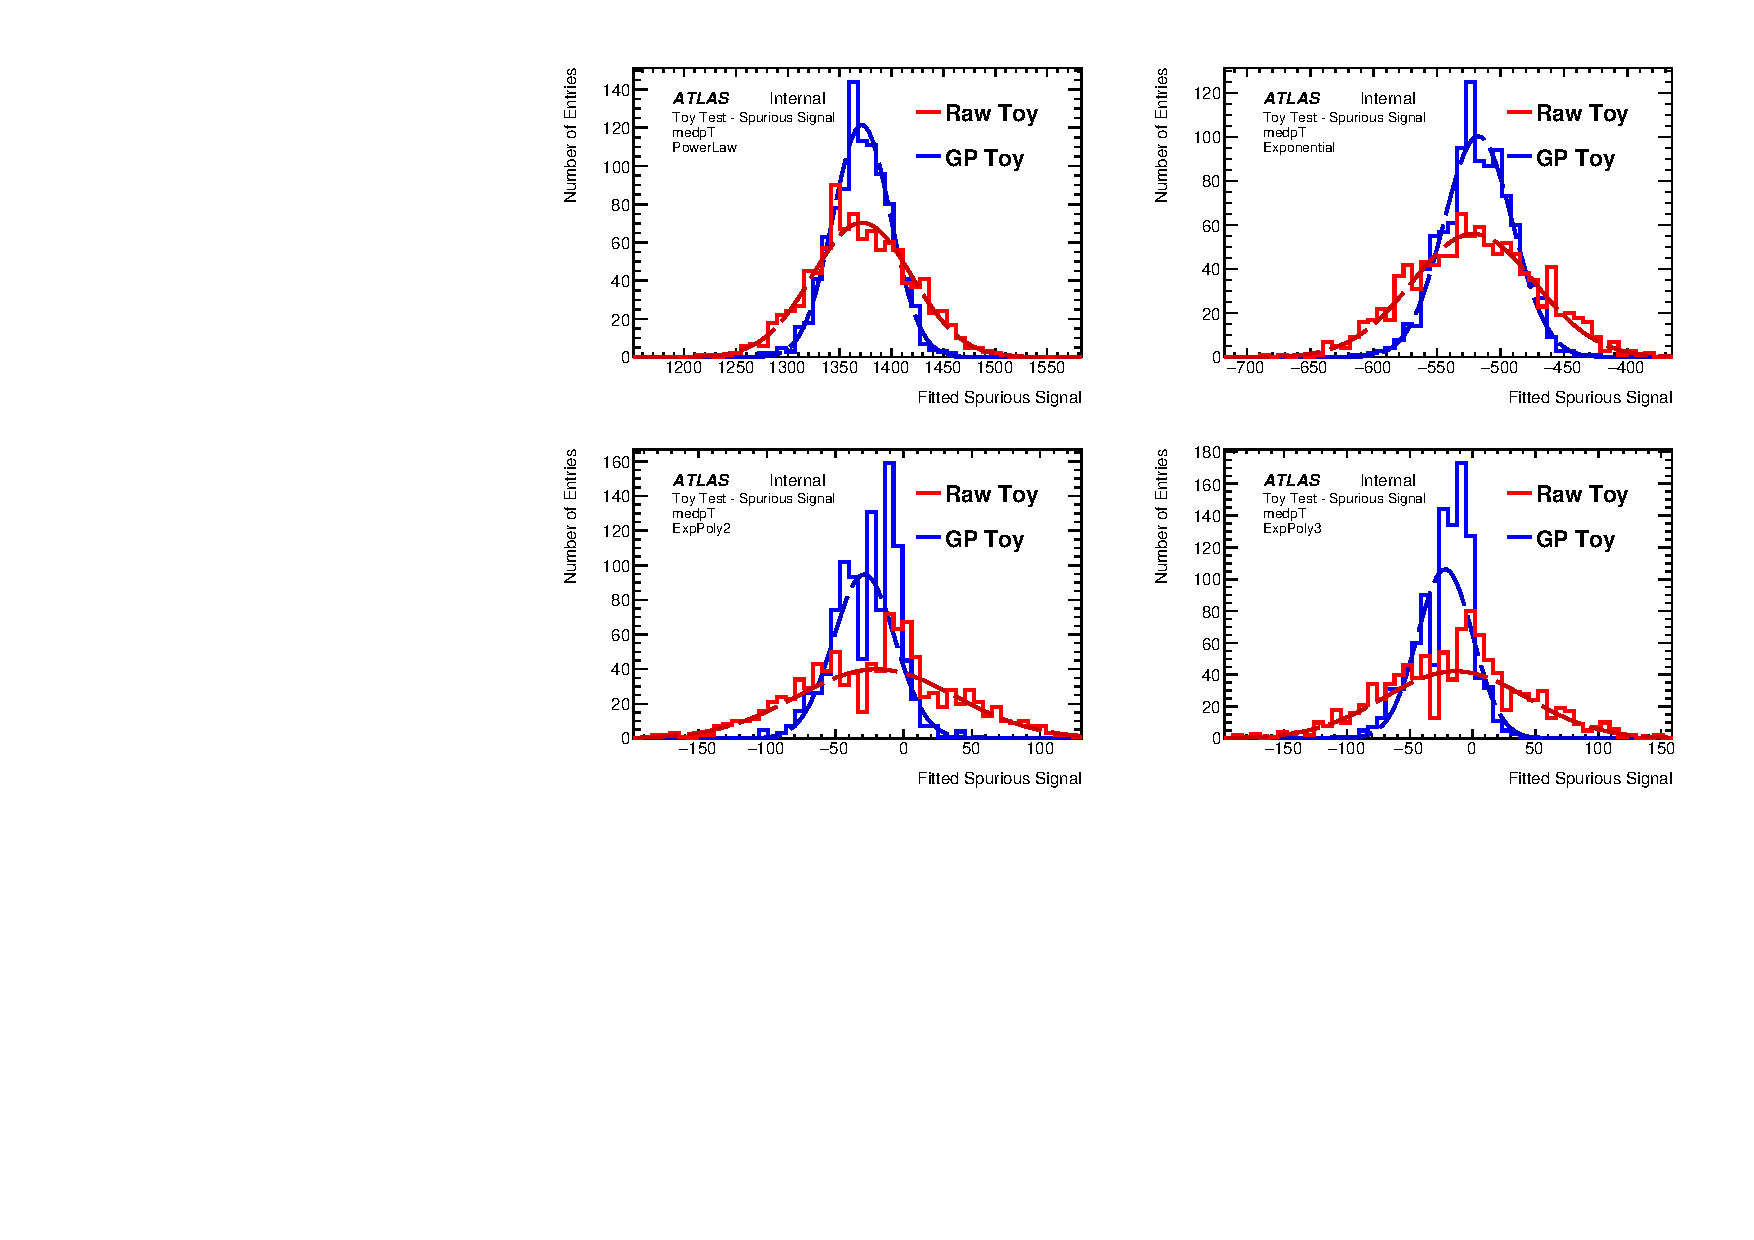
\includegraphics[width=\textwidth]{figures/background/gpr/validation/nominal/ToyTest_FitSigVals_medpT_10M_noSig}   
\caption{The distribution of spurious signal for various functions for both the GPR and raw template, using an expPoly3-derived template. Each toy in this test has 10,000,000 events.}
\label{fig:medpt_10M_noSig}
\end{center}
\end{figure}

\begin{figure} 
\begin{center}
  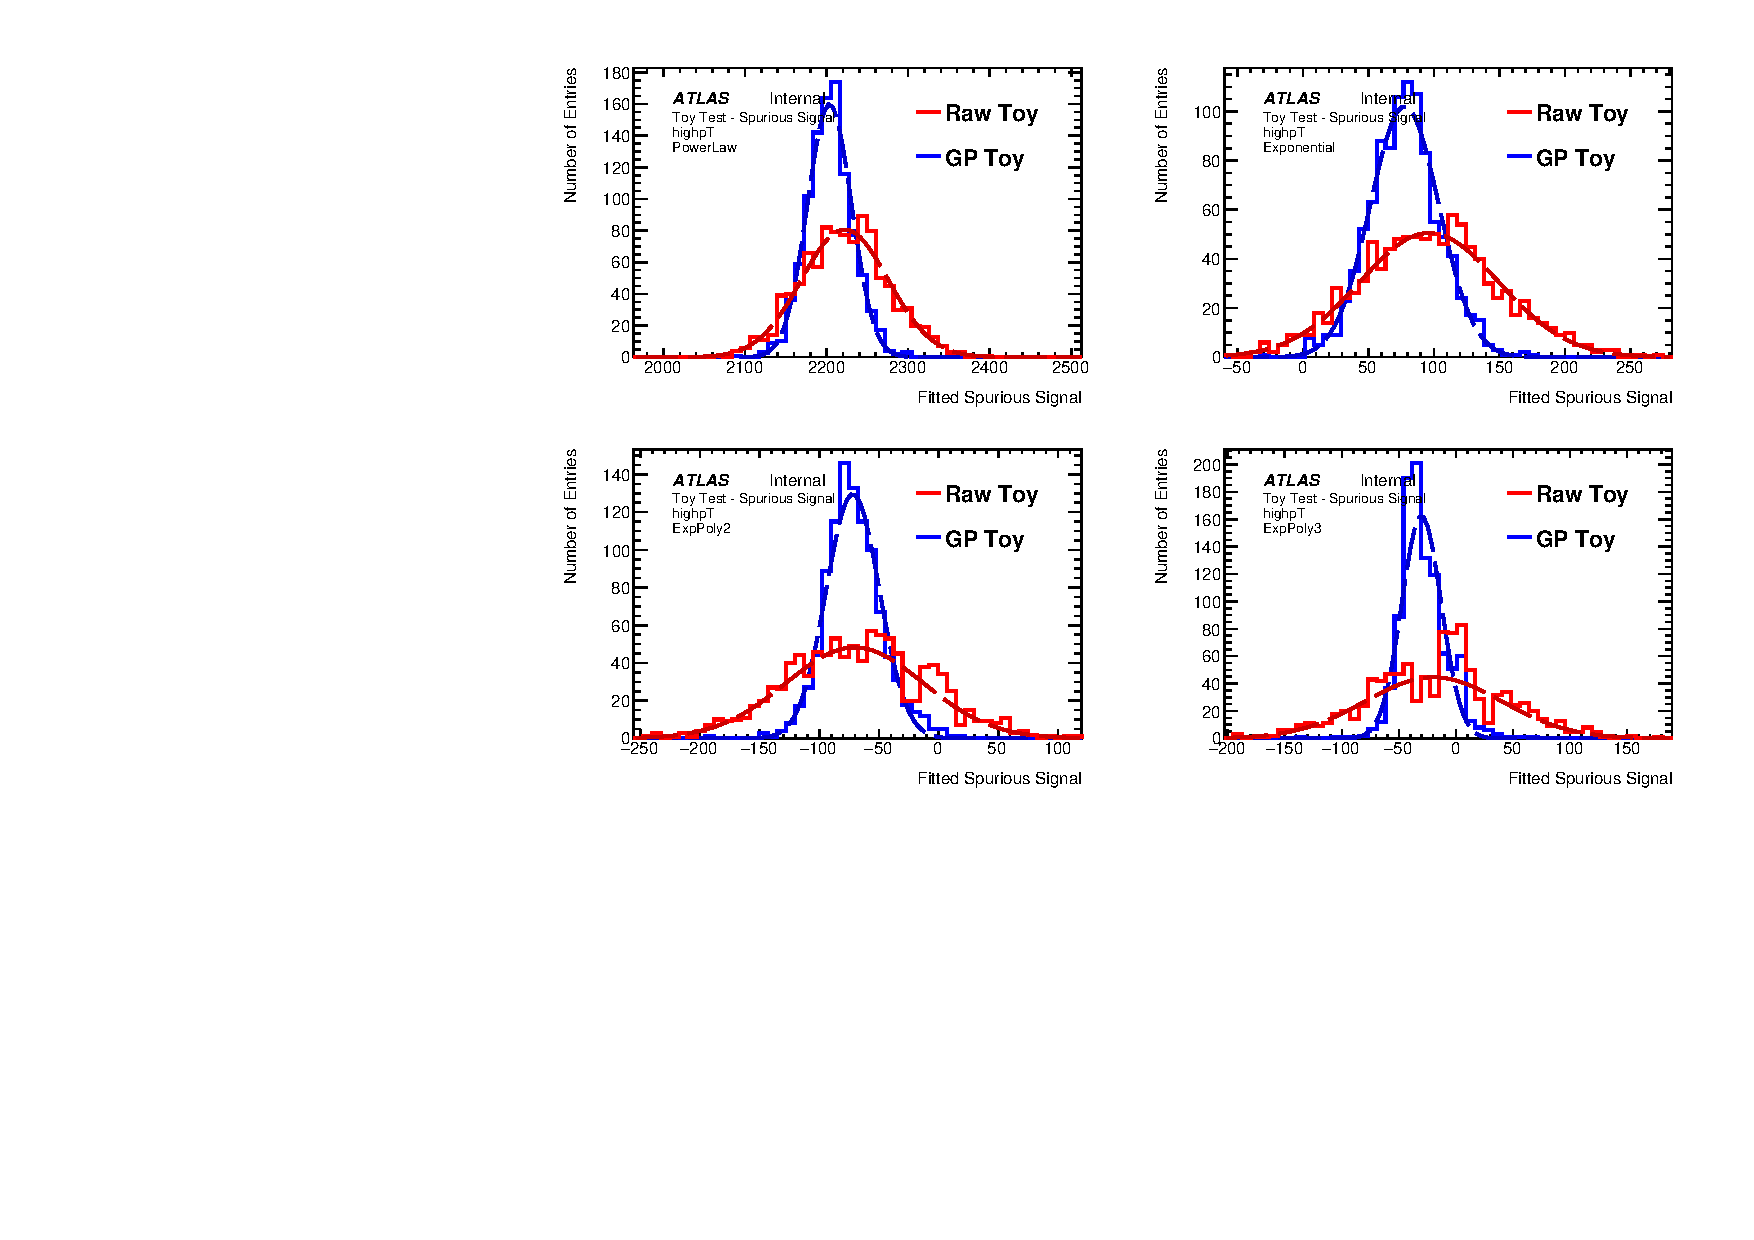
\includegraphics[width=\textwidth]{figures/background/gpr/validation/nominal/ToyTest_FitSigVals_highpT_10M_noSig}   
\caption{The distribution of spurious signal for various functions for both the GPR and raw template, using a different expPoly3-derived template. Each toy in this test has 10,000,000 events.}
\label{fig:highpt_10M_noSig}
\end{center}
\end{figure}

We report the results of the nominal bias study for all categories in the \Tab{\ref{tab:NoSigSS}}. Additionally, we plot the per-toy bias (that is, GP\_SS - Raw\_SS for each toy) for each shape and stat regime.

\begin{landscape}
	\begin{table}
		\centering 
		\resizebox{\linewidth}{!}{
			\begin{tabular}{lcSS
					S[table-format = 3.2, round-mode = places, round-precision = 2]
					S[table-format = 3.2, round-mode = places, round-precision = 2]
					S[table-format = 3.2, round-mode = places, round-precision = 2]
					S[table-format = 3.2, round-mode = places, round-precision = 2]
					S[table-format = 3.2, round-mode = places, round-precision = 2]
					S[table-format = 3.2, round-mode = places, round-precision = 2]
				}
				Nominal                   & N\_sig & {\makecell{Unweighted \\ Events}} & {\makecell{Bkg events \\ weighted}} & {Mean SS\_raw}         & {Mean SS\_GPR}        & {\makecell{GP-Raw: \\Bias, Mean}} & {Sigma Toy}         & {Sigma GPR}          & {Bias/sigma(SS\_raw)} \\
				\hline
				Fit: Exp         &        &                     &                       &                        &                       &                      &                     &                      &                       \\
				Generating: Exp2  &        &                     &                       &                        &                       &                      &                     &                      &                       \\
				low10                  &   0    & e1                  & 0.4                   & -0.0856086392657038    & -0.0198181405147273   & 0.065790498750977    & 0.179605304942675   & 0.0804227608321356   & 0.366305988411506     \\
				low100                 &   0    & e2                  & 4                     & -0.00456279273313931   & -0.06339782409475457  & -0.058835031361615   & 0.15876721225261617 & 0.5777433151077007   & -0.370574191779611    \\
				low1k                  &   0    & e3                  & 4e1                   & -0.08312535796905889   & 0.016139400710191487  & 0.09926475867925     & 0.5155595221854518  & 0.22290210095525473  & 0.19253792124422      \\
				low10k                 &   0    & e4                  & 4e2                   & -0.8088403732000055    & -0.5714771528789513   & 0.237363220321054    & 1.6192934455040988  & 0.7940658071133893   & 0.146584438404344     \\
				low100k                &   0    & e5                  & 4e3                   & -8.662558651490635     & -7.180045066316387    & 1.48251358517425     & 5.2208056521806565  & 2.0602948862549058   & 0.283962607295106     \\
				low1M                  &   0    & e6                  & 4e4                   & -87.69944954490472     & -85.6101975590245     & 2.08925198588022     & 15.669450391614046  & 9.115771729935428    & 0.133332818552356     \\
				low10M                 &   0    & e7                  & 4e5                   & -871.7509377878234     & -876.5849772067857    & -4.83403941896222    & 50.31897375421032   & 29.77441032102435    & -0.096067925442493    \\
				\hline
				Fit: Exp2        &        &                     &                       &                        &                       &                      &                     &                      &                       \\
				Generating: Exp3 &        &                     &                       &                        &                       &                      &                     &                      &                       \\
				med10                  &   0    & e1                  & 0.4                   & -0.10147202640635238   & -0.007495570836160461 & 0.093976455570192    & 0.1899571908509915  & 0.0505766175720417   & 0.494724391054562     \\
				med100                 &   0    & e2                  & 4                     & -0.0009487144527428039 & 0.03673375124126233   & 0.037682465694005    & 0.174682427170514   & 0.23577418182938328  & 0.215719842598831     \\
				med1k                  &   0    & e3                  & 4e1                   & -0.011218465820916826  & -0.038589743657067826 & -0.027371277836151   & 0.561639982124615   & 0.23291724529751529  & -0.048734560763657    \\
				med10k                 &   0    & e4                  & 4e2                   & -0.01188562598373835   & -0.025960990531341054 & -0.014075364547603   & 1.784473152441334   & 0.3852513961827399   & -0.007887686361852    \\
				med100k                &   0    & e5                  & 4e3                   & -0.27118453498416467   & -0.8887620543116782   & -0.617577519327513   & 5.684209055204971   & 1.640510314152104    & -0.108647925037522    \\
				med1M                  &   0    & e6                  & 4e4                   & -1.9534510830223808    & -4.959142177670772    & -3.00569109464839    & 16.902135565317487  & 5.691272889007479    & -0.177829072724748    \\
				med10M                 &   0    & e7                  & 4e5                   & -20.42989690333931     & -26.755933120427304   & -6.326036217088      & 55.28558245403774   & 23.0604489566008     & -0.114424700550948    \\
				\hline
				Fit: Exp2        &        &                     &                       &                        &                       &                      &                     &                      &                       \\
				Generating: Exp3 &        &                     &                       &                        &                       &                      &                     &                      &                       \\
				high10                 &   0    & e1                  & 0.4                   & -0.10424559123307484   & -0.007415442347673825 & 0.096830148885401    & 0.19245261858875531 & 0.037550491861219434 & 0.503137601324686     \\
				high100                &   0    & e2                  & 4                     & -0.012054685573784028  & 0.01916704871163027   & 0.031221734285414    & 0.18434206816345447 & 0.24863747745658435  & 0.16936847132327      \\
				high1k                 &   0    & e3                  & 4e1                   & 0.00029766977634685787 & -0.03323398495940897  & -0.033531654735756   & 0.5495740987559312  & 0.31722528484167756  & -0.061013892051429    \\
				high10k                &   0    & e4                  & 4e2                   & -0.13224523509238087   & -0.13561317449969687  & -0.003367939407316   & 1.7367933808521807  & 0.38522893906701317  & -0.00193917102889     \\
				high100k               &   0    & e5                  & 4e3                   & -0.9128795645403252    & -1.6253716695465354   & -0.71249210500621    & 5.466963438977402   & 1.8602563479729348   & -0.130326846513443    \\
				high1M                 &   0    & e6                  & 4e4                   & -6.722672666705272     & -11.328761840185077   & -4.60608917347981    & 17.919147598803733  & 10.217042596843571   & -0.257048453230404    \\
				high10M                &   0    & e7                  & 4e5                   & -67.98514243446012     & -71.0056531649924     & -3.02051073053228    & 58.72969029815181   & 24.19364408740454    & -0.051430728055914 \\
				\hline
			\end{tabular}
		}
		\caption{Spurious signal means and widths for the three test functional-form distributions for a range of different template statistics.}
		\label{tab:NoSigSS}
	\end{table}	
\end{landscape}


\begin{figure} 
\begin{center}
  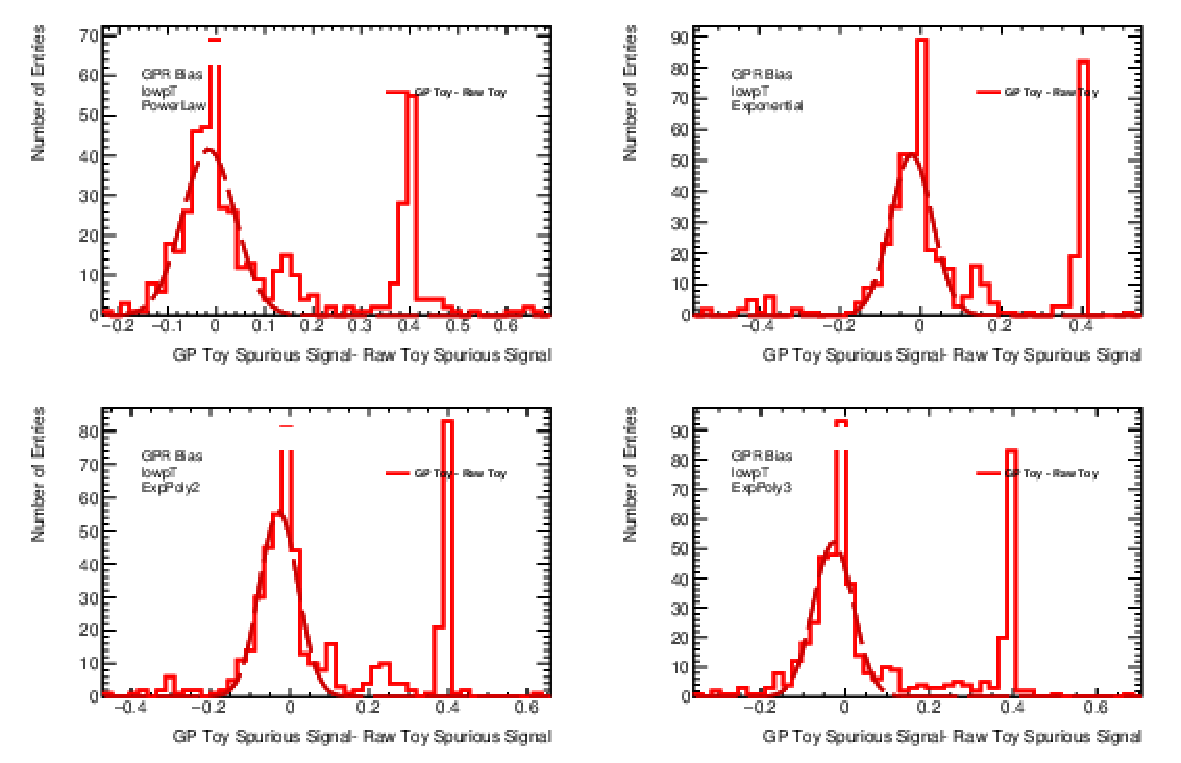
\includegraphics[width=\textwidth]{figures/background/gpr/validation/nominal/ToyTest_FitSigBiases_lowpT_10_noSig}   
\caption{The per-toy bias (GP Spurious Signal - Raw Spurious Signal), using an expPoly2-derived template. Each toy in this test has 10 events.}
\label{fig:bias_lowpt_10_noSig}
\end{center}
\end{figure}

\begin{figure} 
\begin{center}
  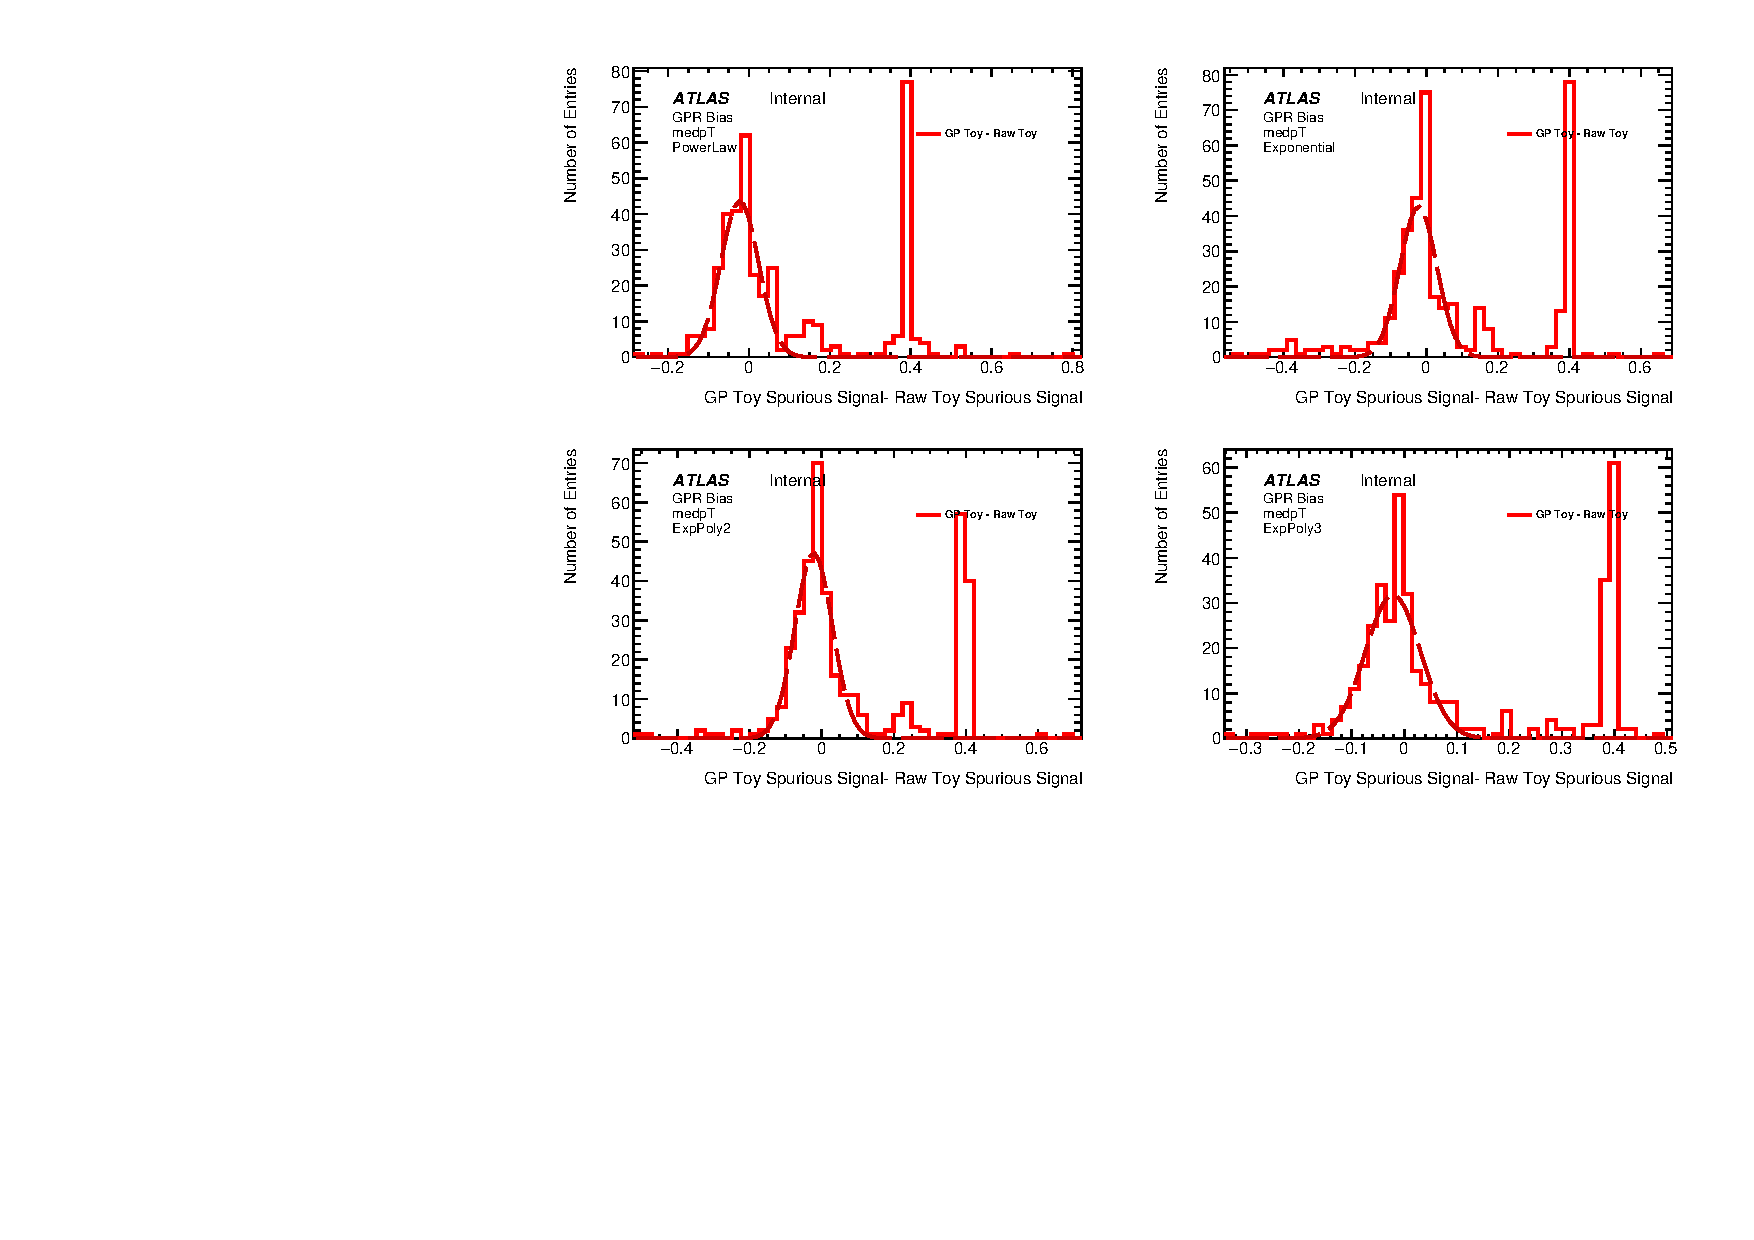
\includegraphics[width=\textwidth]{figures/background/gpr/validation/nominal/ToyTest_FitSigBiases_medpT_10_noSig}   
\caption{The per-toy bias (GP Spurious Signal - Raw Spurious Signal), using an expPoly3-derived template. Each toy in this test has 10 events.}
\label{fig:bias_medpt_10_noSig}
\end{center}
\end{figure}

\begin{figure} 
\begin{center}
  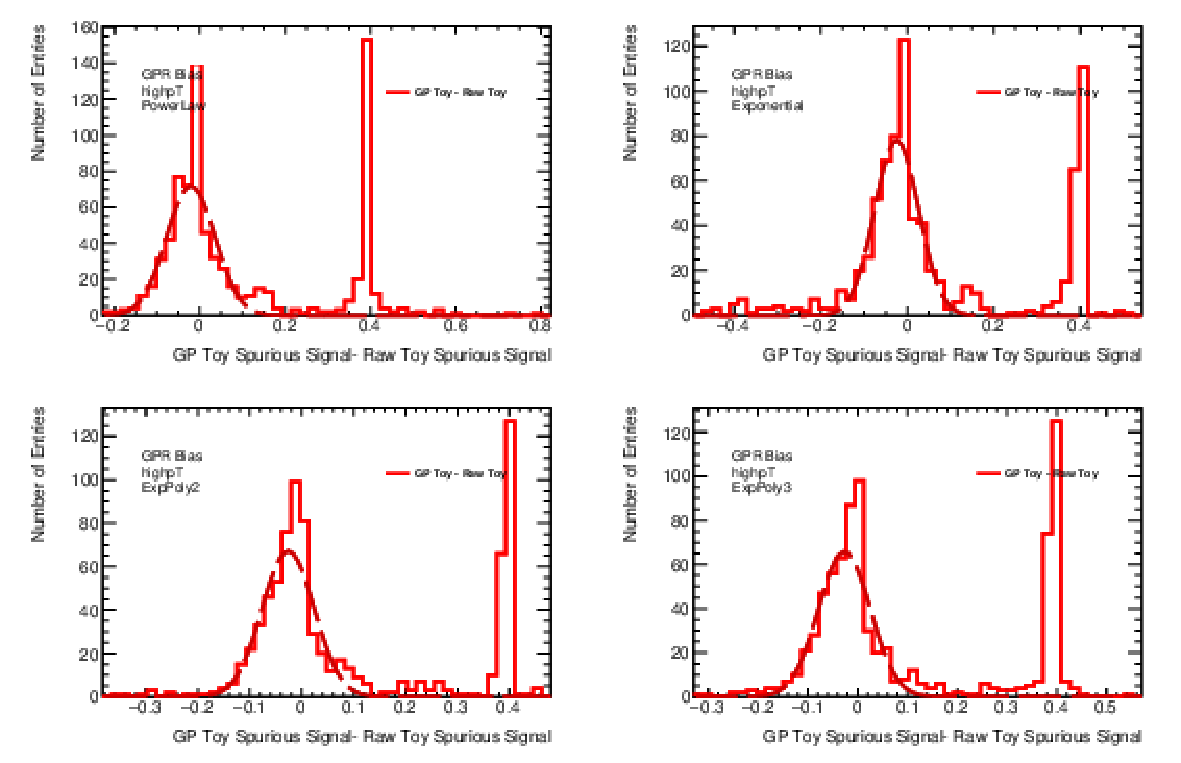
\includegraphics[width=\textwidth]{figures/background/gpr/validation/nominal/ToyTest_FitSigBiases_highpT_10_noSig}   
\caption{The per-toy bias (GP Spurious Signal - Raw Spurious Signal), using a different expPoly3-derived template. Each toy in this test has 10 events.}
\label{fig:bias_highpt_10_noSig}
\end{center}
\end{figure}

\begin{figure} 
\begin{center}
  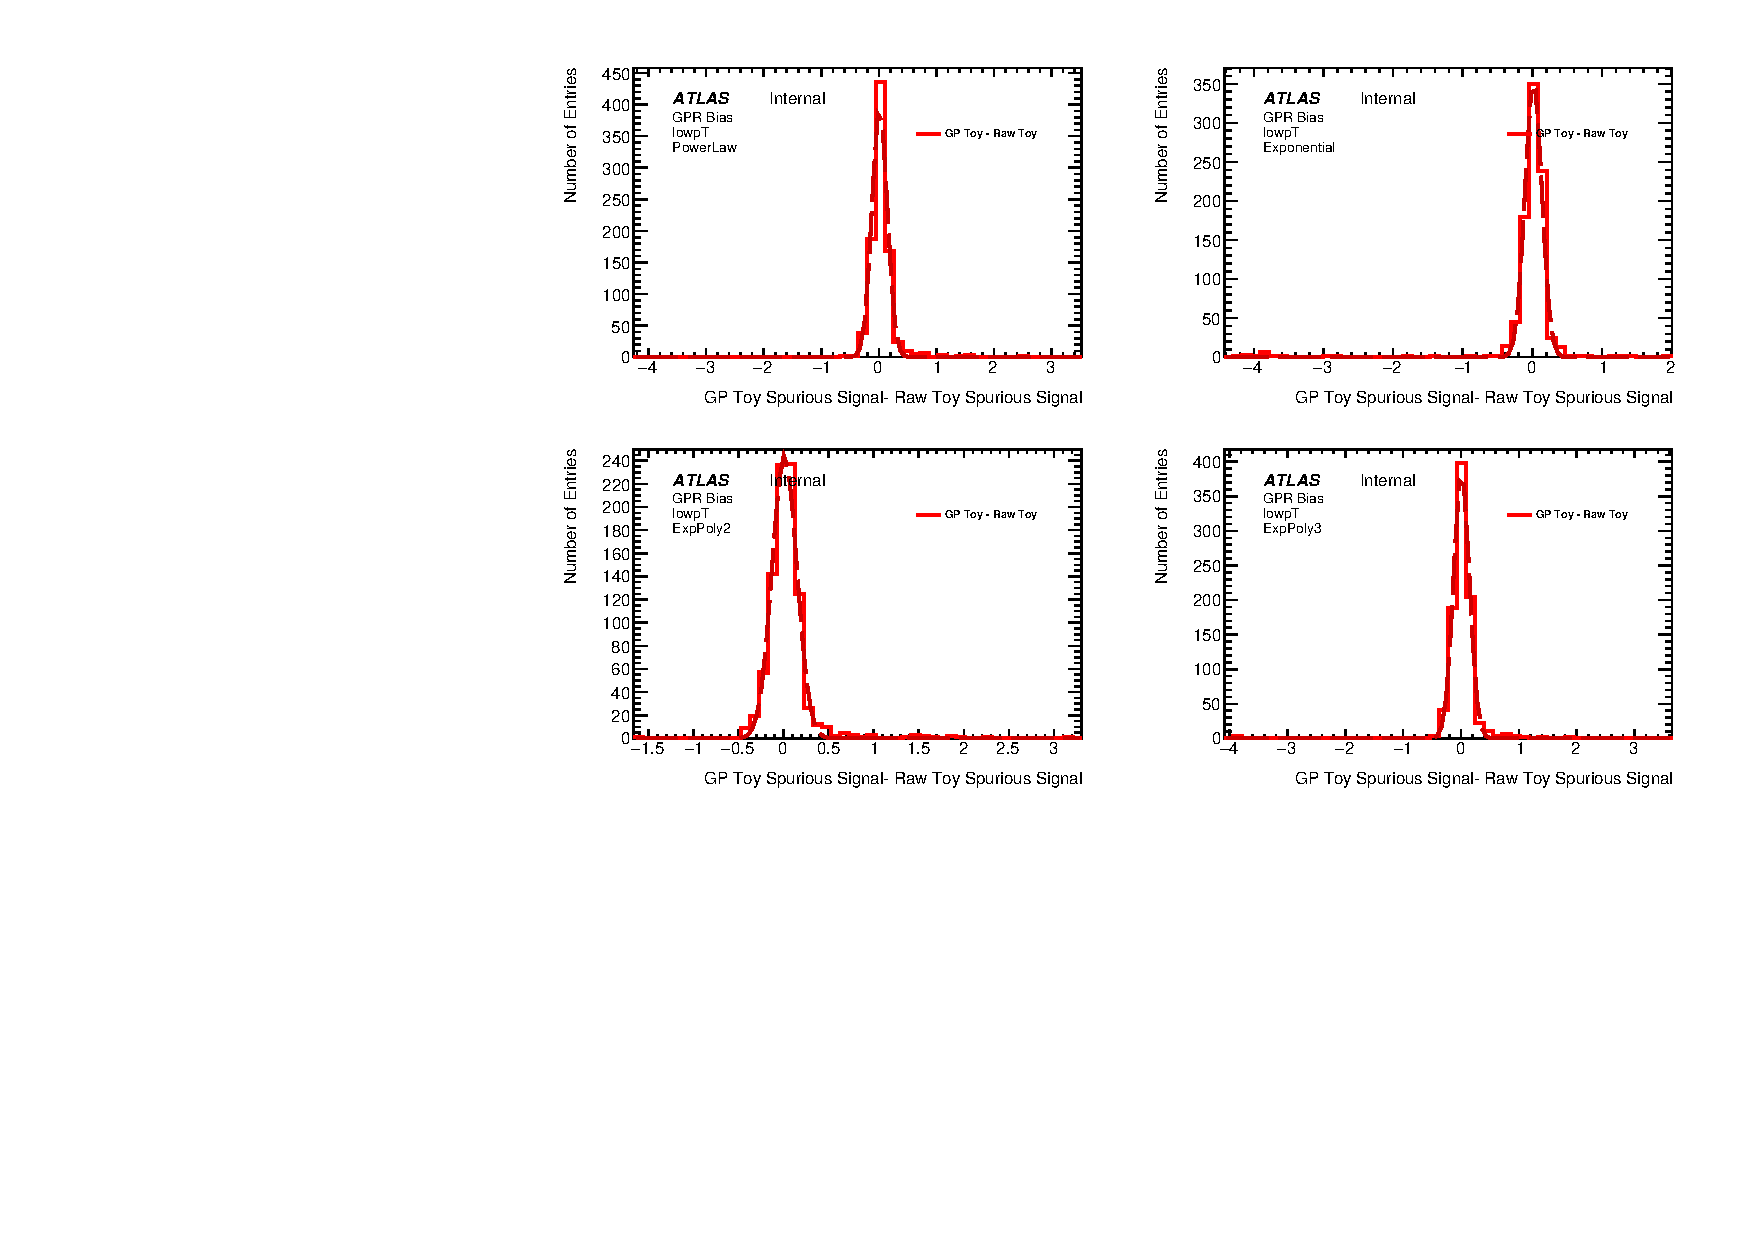
\includegraphics[width=\textwidth]{figures/background/gpr/validation/nominal/ToyTest_FitSigBiases_lowpT_100_noSig}   
\caption{The per-toy bias (GP Spurious Signal - Raw Spurious Signal), using an expPoly2-derived template. Each toy in this test has 100 events.}
\label{fig:bias_lowpt_100_noSig}
\end{center}
\end{figure}

\begin{figure} 
\begin{center}
  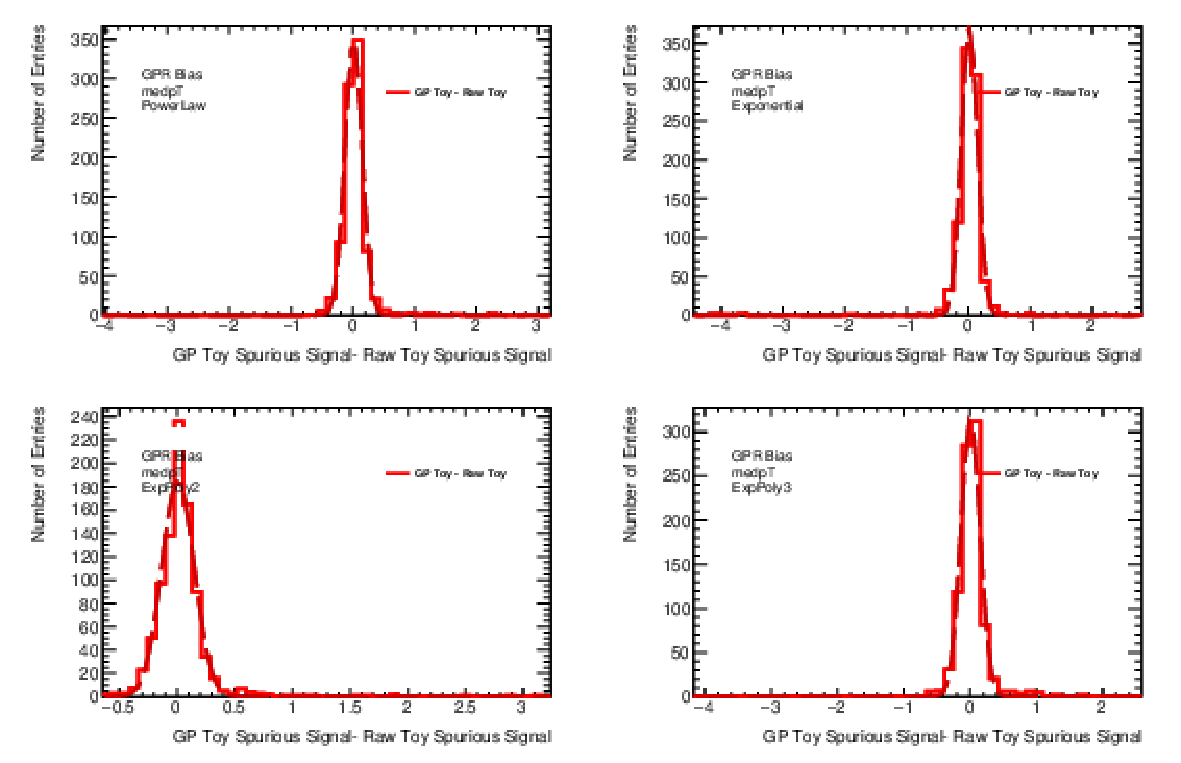
\includegraphics[width=\textwidth]{figures/background/gpr/validation/nominal/ToyTest_FitSigBiases_medpT_100_noSig}   
\caption{The per-toy bias (GP Spurious Signal - Raw Spurious Signal), using an expPoly3-derived template. Each toy in this test has 100 events.}
\label{fig:bias_medpt_100_noSig}
\end{center}
\end{figure}

\begin{figure} 
\begin{center}
  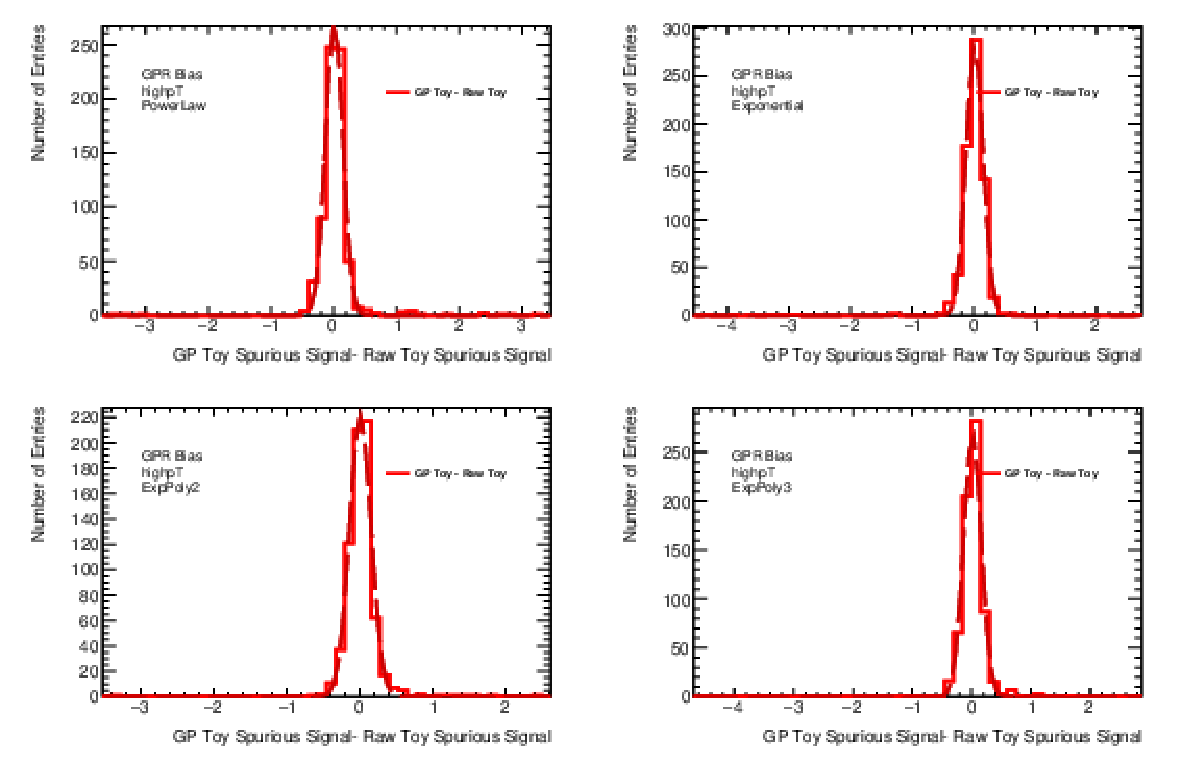
\includegraphics[width=\textwidth]{figures/background/gpr/validation/nominal/ToyTest_FitSigBiases_highpT_100_noSig}   
\caption{The per-toy bias (GP Spurious Signal - Raw Spurious Signal), using a different expPoly3-derived template. Each toy in this test has 100 events.}
\label{fig:bias_highpt_100_noSig}
\end{center}
\end{figure}

\begin{figure} 
\begin{center}
  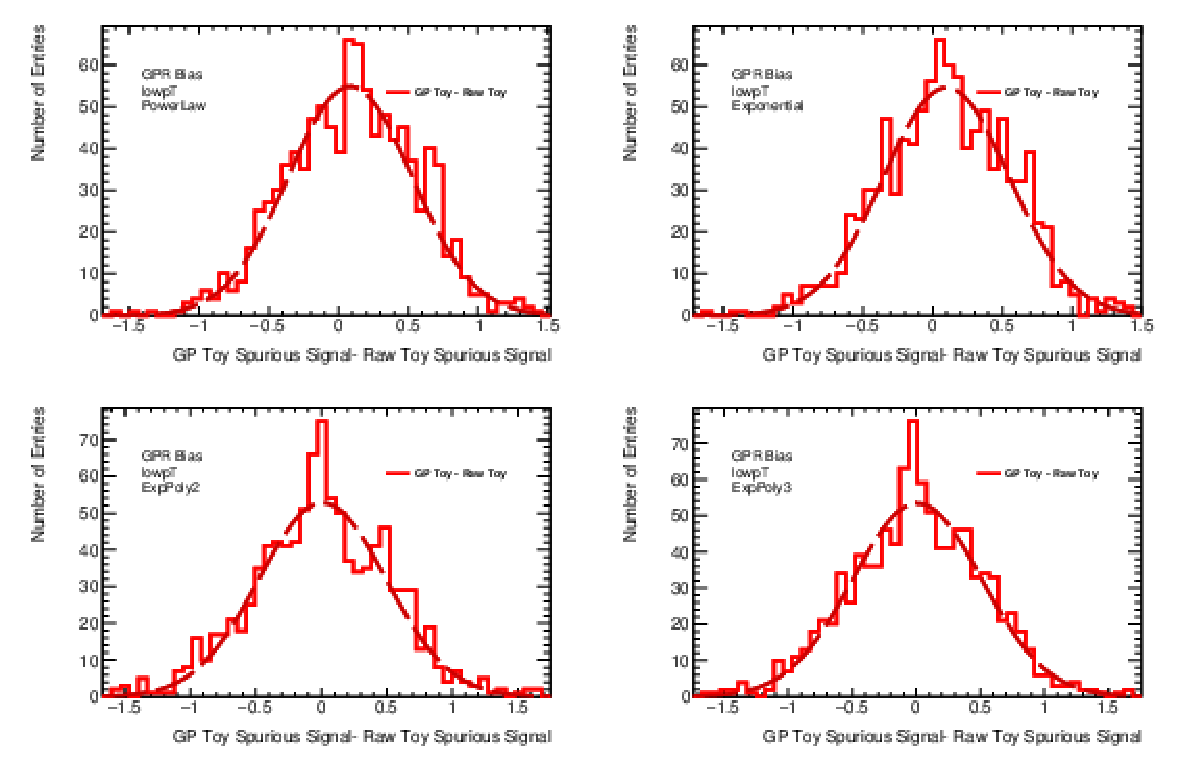
\includegraphics[width=\textwidth]{figures/background/gpr/validation/nominal/ToyTest_FitSigBiases_lowpT_1000_noSig}   
\caption{The per-toy bias (GP Spurious Signal - Raw Spurious Signal), using an expPoly2-derived template. Each toy in this test has 1000 events.}
\label{fig:bias_lowpt_1000_noSig}
\end{center}
\end{figure}

\begin{figure} 
\begin{center}
  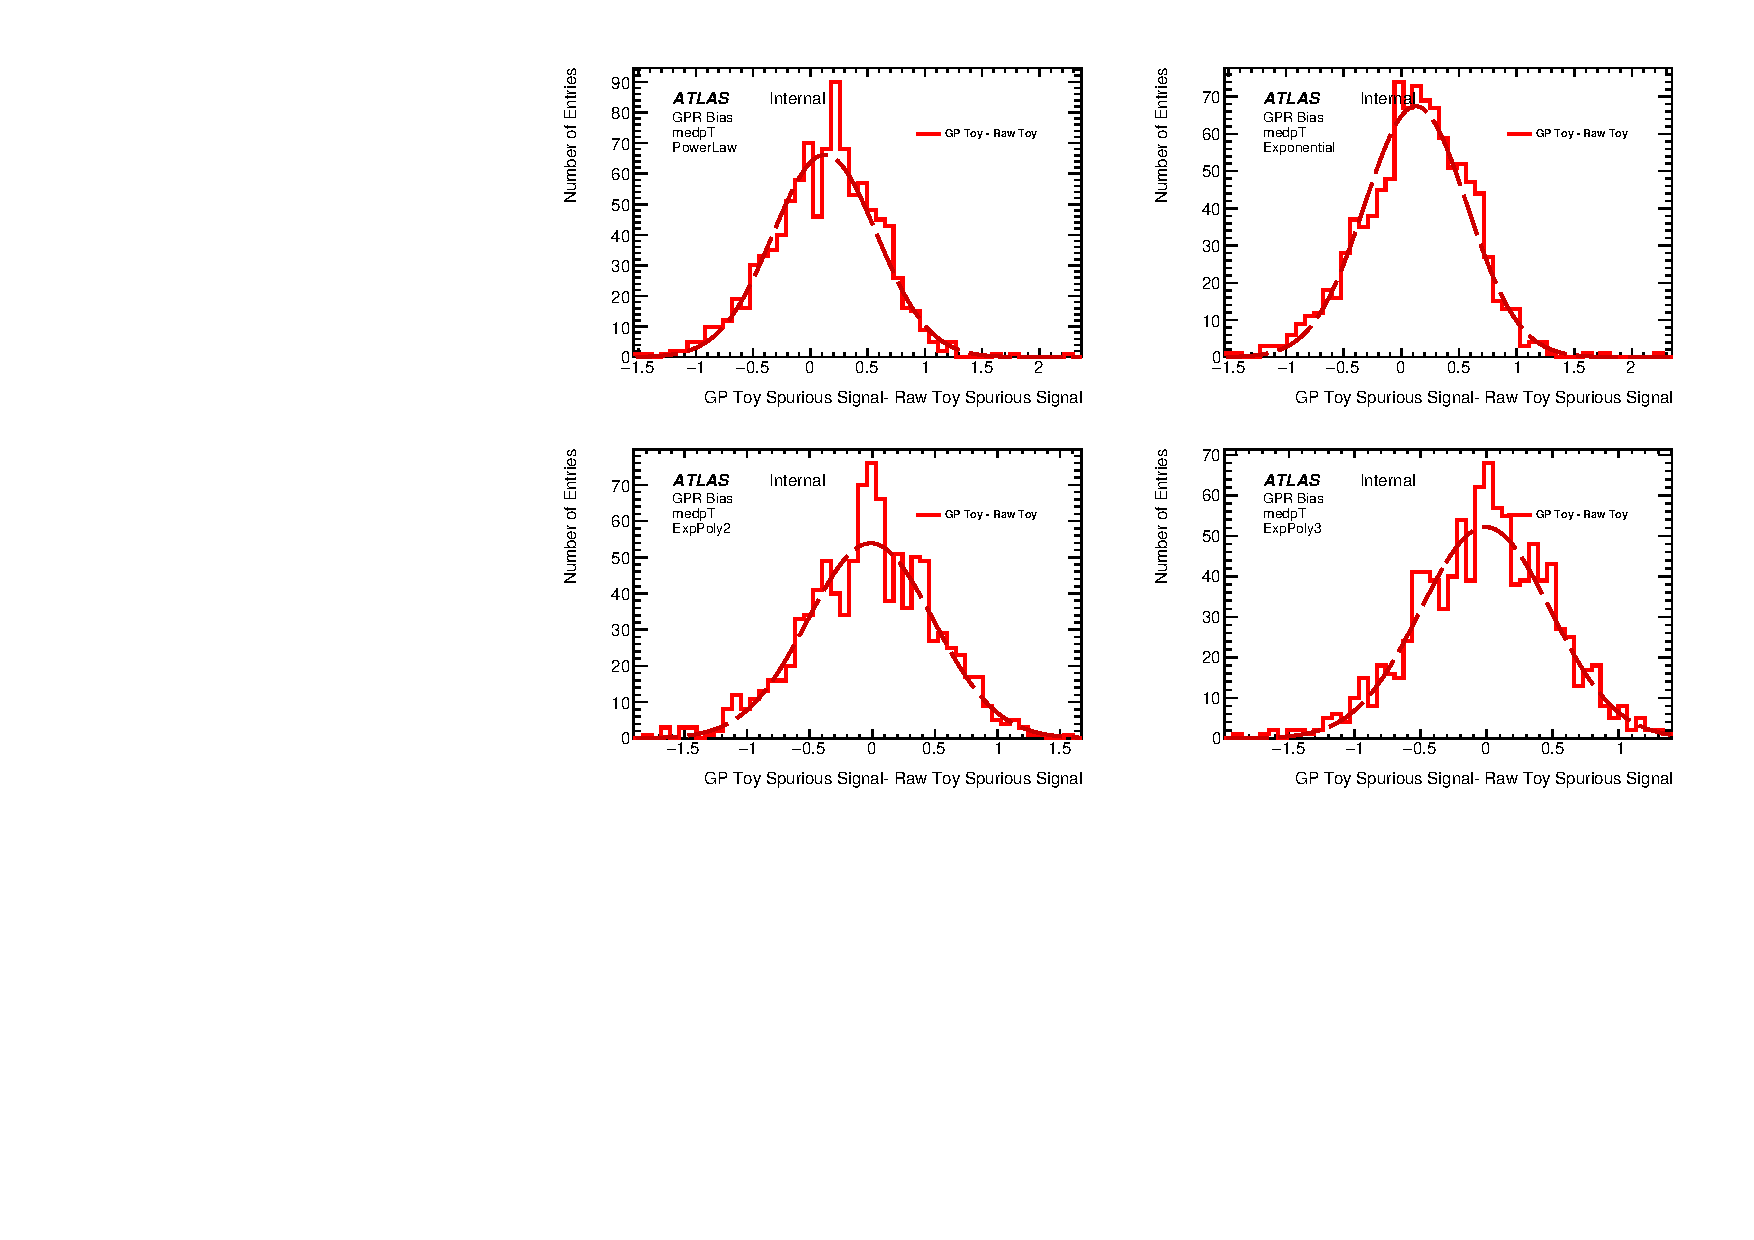
\includegraphics[width=\textwidth]{figures/background/gpr/validation/nominal/ToyTest_FitSigBiases_medpT_1000_noSig}   
\caption{The per-toy bias (GP Spurious Signal - Raw Spurious Signal), using an expPoly3-derived template. Each toy in this test has 1000 events.}
\label{fig:bias_medpt_1000_noSig}
\end{center}
\end{figure}

\begin{figure} 
\begin{center}
  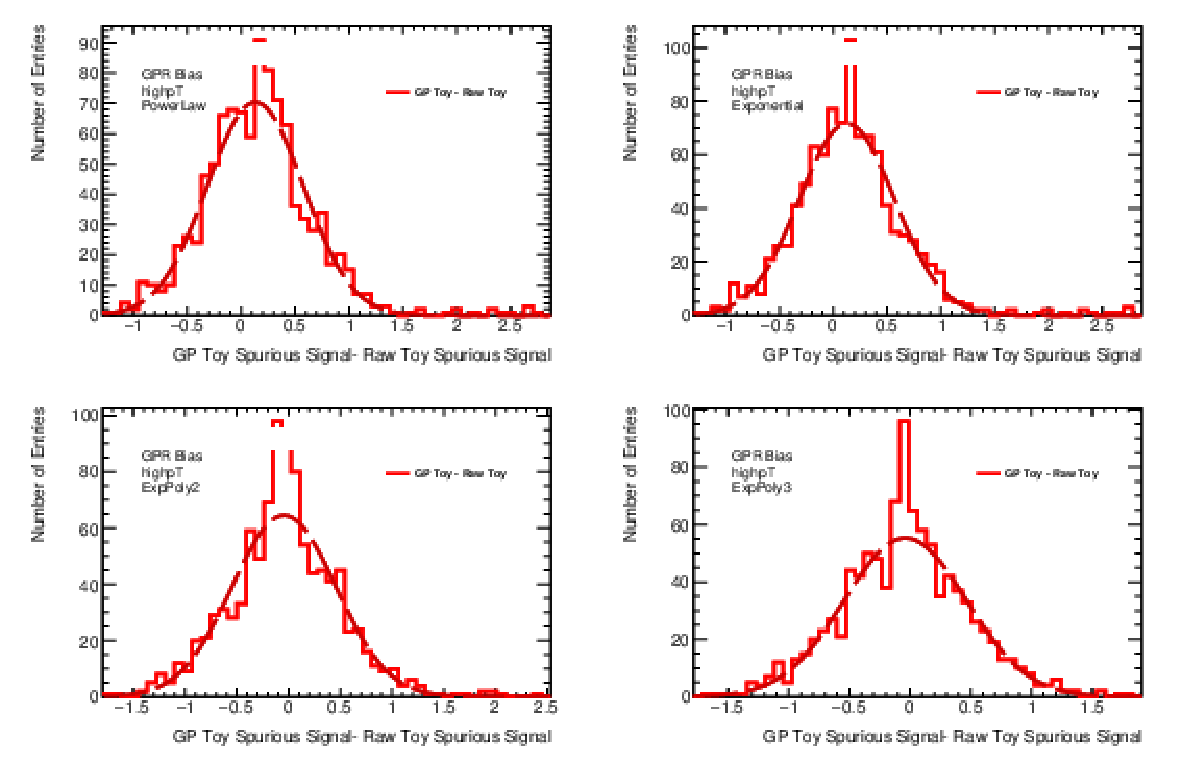
\includegraphics[width=\textwidth]{figures/background/gpr/validation/nominal/ToyTest_FitSigBiases_highpT_1000_noSig}   
\caption{The per-toy bias (GP Spurious Signal - Raw Spurious Signal), using a different expPoly3-derived template. Each toy in this test has 1000 events.}
\label{fig:bias_highpt_1000_noSig}
\end{center}
\end{figure}

\begin{figure} 
\begin{center}
  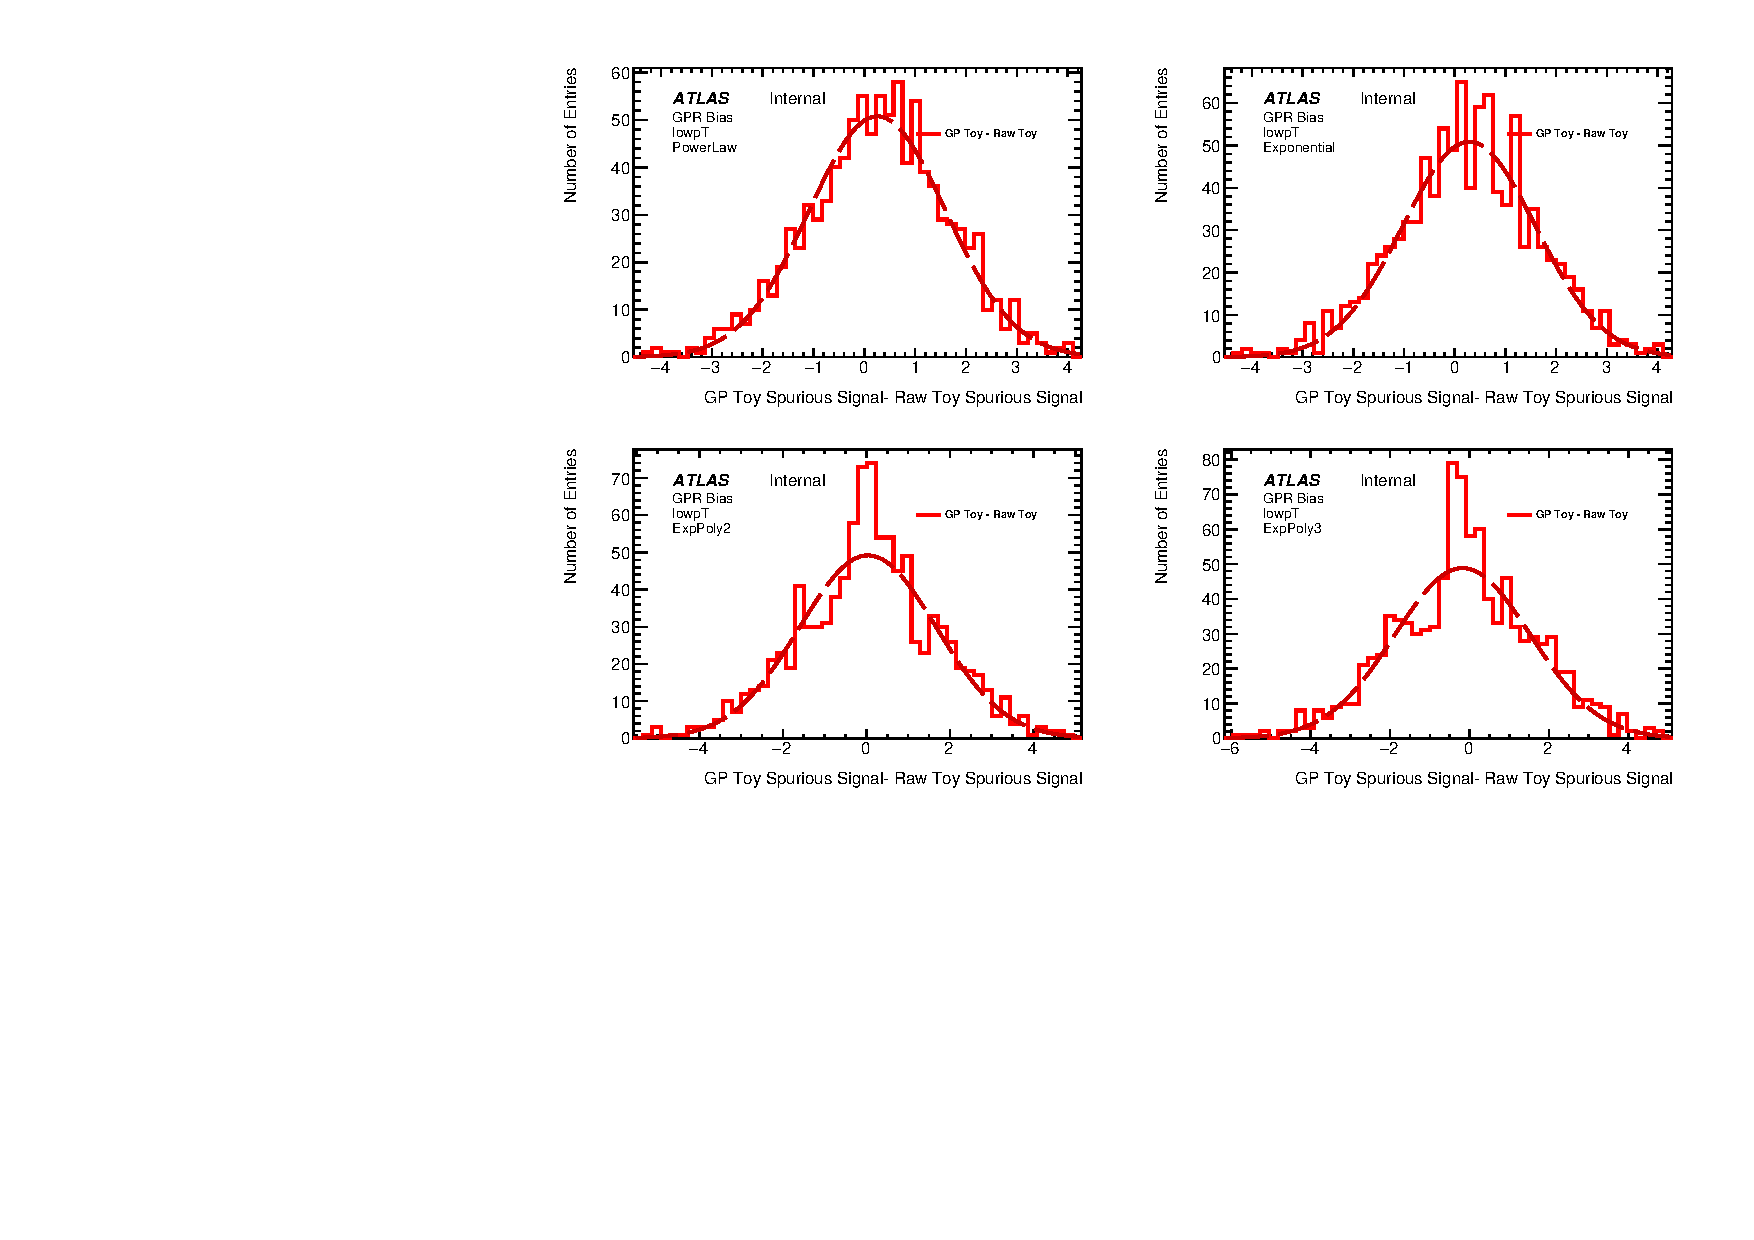
\includegraphics[width=\textwidth]{figures/background/gpr/validation/nominal/ToyTest_FitSigBiases_lowpT_10k_noSig}   
\caption{The per-toy bias (GP Spurious Signal - Raw Spurious Signal), using an expPoly2-derived template. Each toy in this test has 10k events.}
\label{fig:bias_lowpt_10k_noSig}
\end{center}
\end{figure}

\begin{figure} 
\begin{center}
  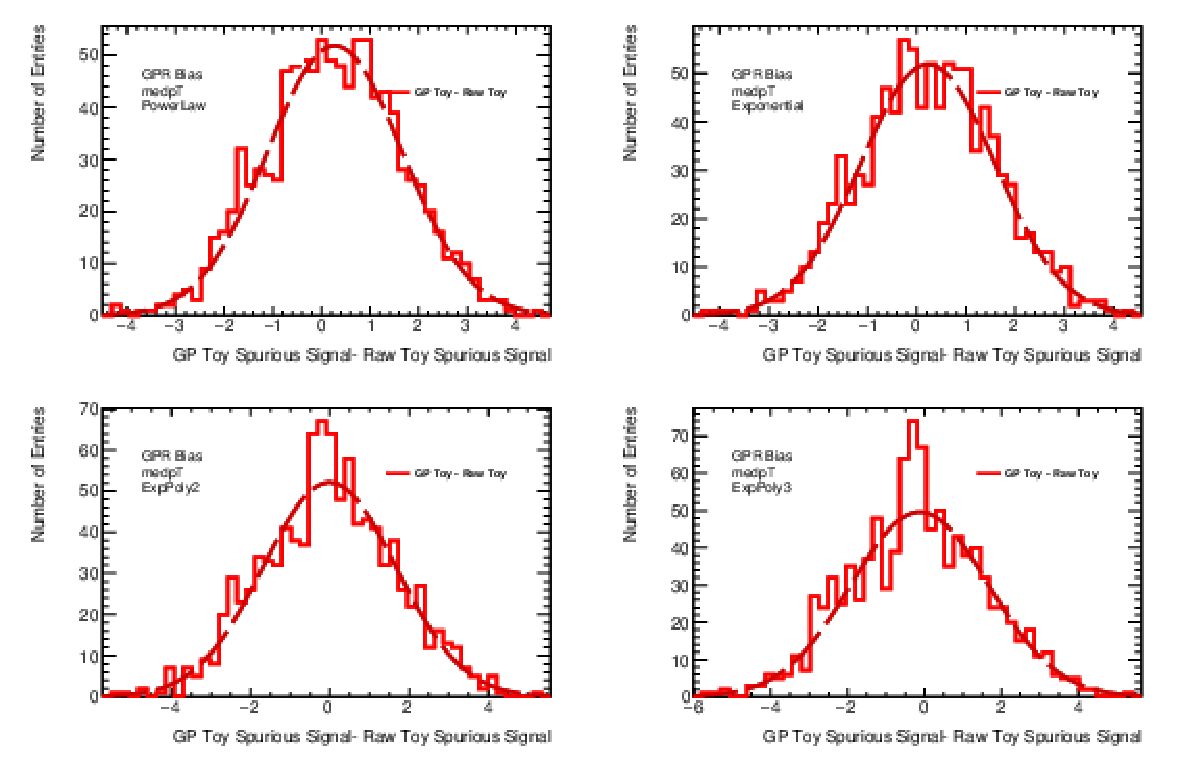
\includegraphics[width=\textwidth]{figures/background/gpr/validation/nominal/ToyTest_FitSigBiases_medpT_10k_noSig}   
\caption{The per-toy bias (GP Spurious Signal - Raw Spurious Signal), using an expPoly3-derived template. Each toy in this test has 10k events.}
\label{fig:bias_medpt_10k_noSig}
\end{center}
\end{figure}

\begin{figure} 
\begin{center}
  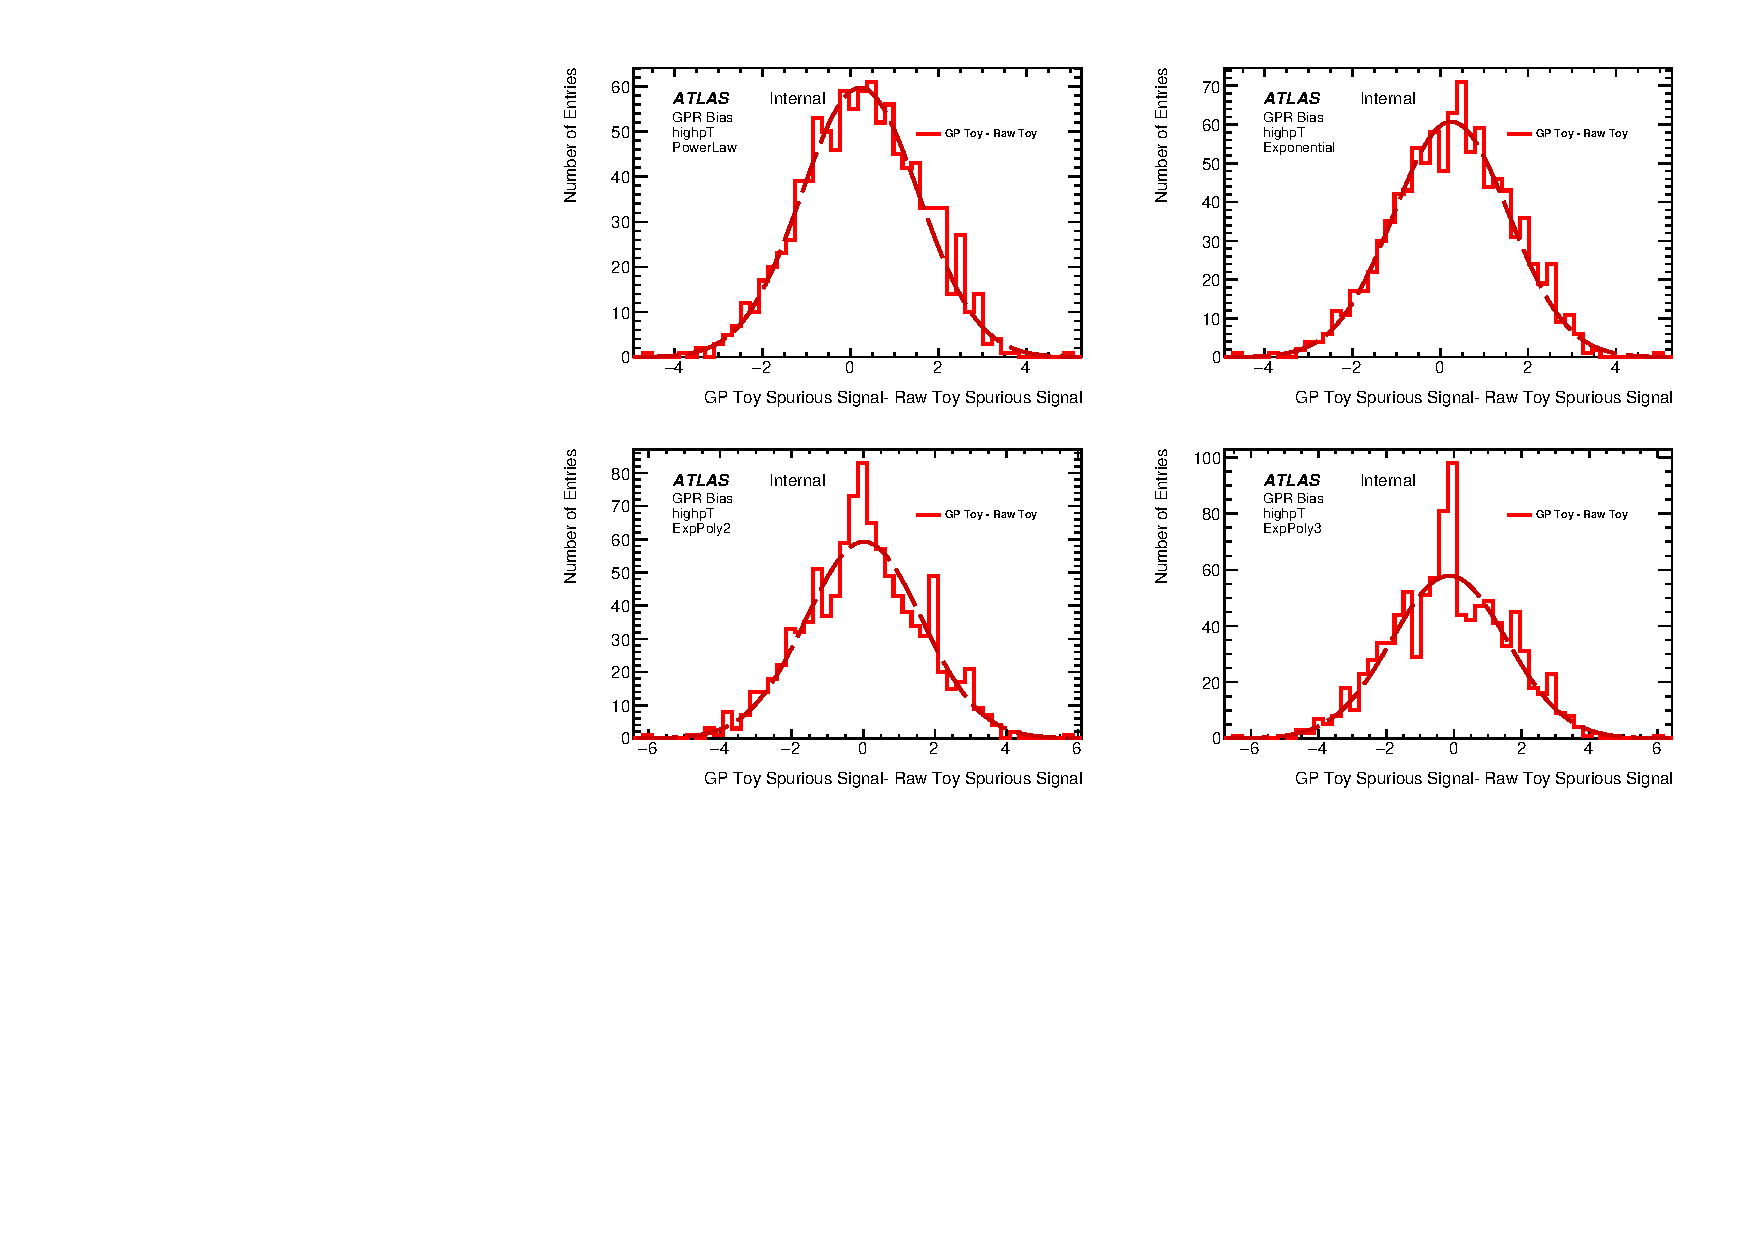
\includegraphics[width=\textwidth]{figures/background/gpr/validation/nominal/ToyTest_FitSigBiases_highpT_10k_noSig}   
\caption{The per-toy bias (GP Spurious Signal - Raw Spurious Signal), using a different expPoly3-derived template. Each toy in this test has 10k events.}
\label{fig:bias_highpt_10k_noSig}
\end{center}
\end{figure}

\begin{figure} 
\begin{center}
  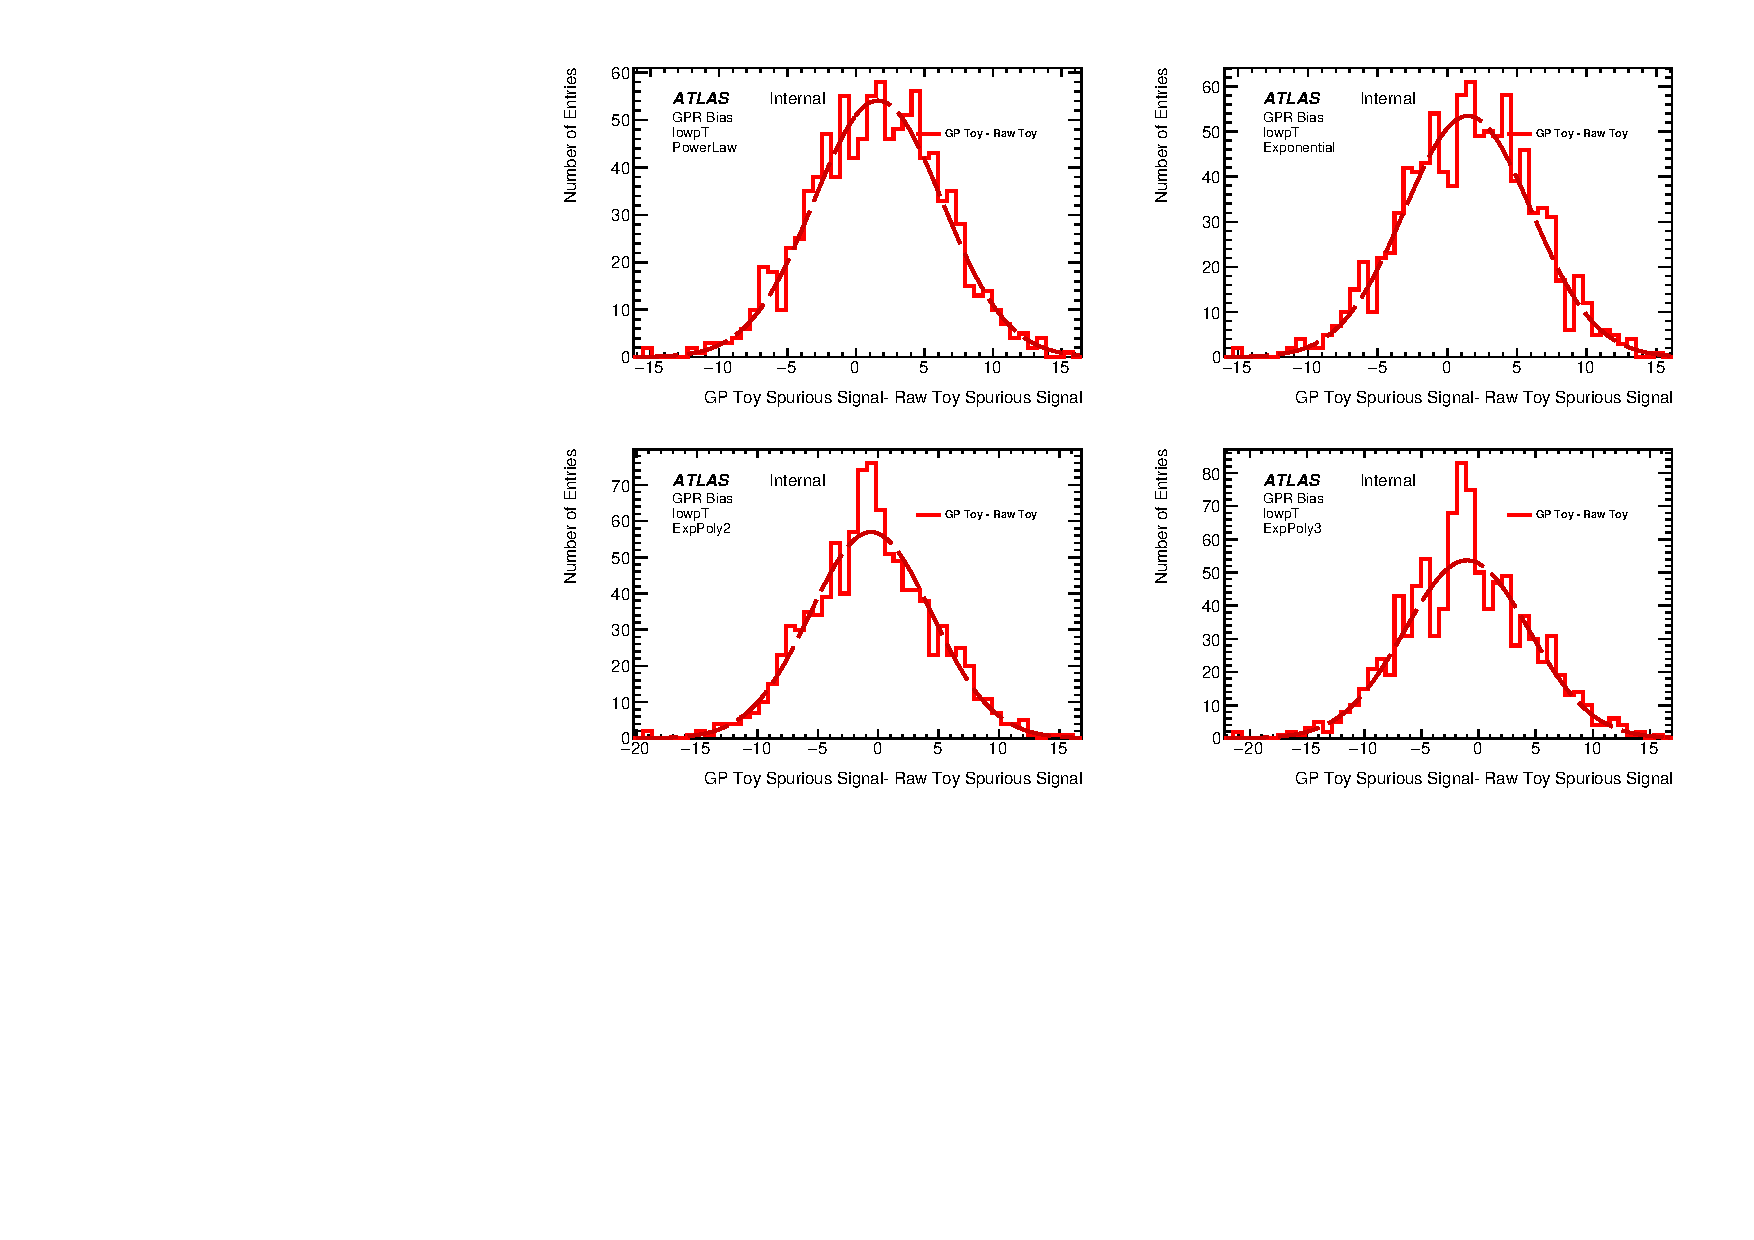
\includegraphics[width=\textwidth]{figures/background/gpr/validation/nominal/ToyTest_FitSigBiases_lowpT_100k_noSig}   
\caption{The per-toy bias (GP Spurious Signal - Raw Spurious Signal), using an expPoly2-derived template. Each toy in this test has 100k events.}
\label{fig:bias_lowpt_100k_noSig}
\end{center}
\end{figure}

\begin{figure} 
\begin{center}
  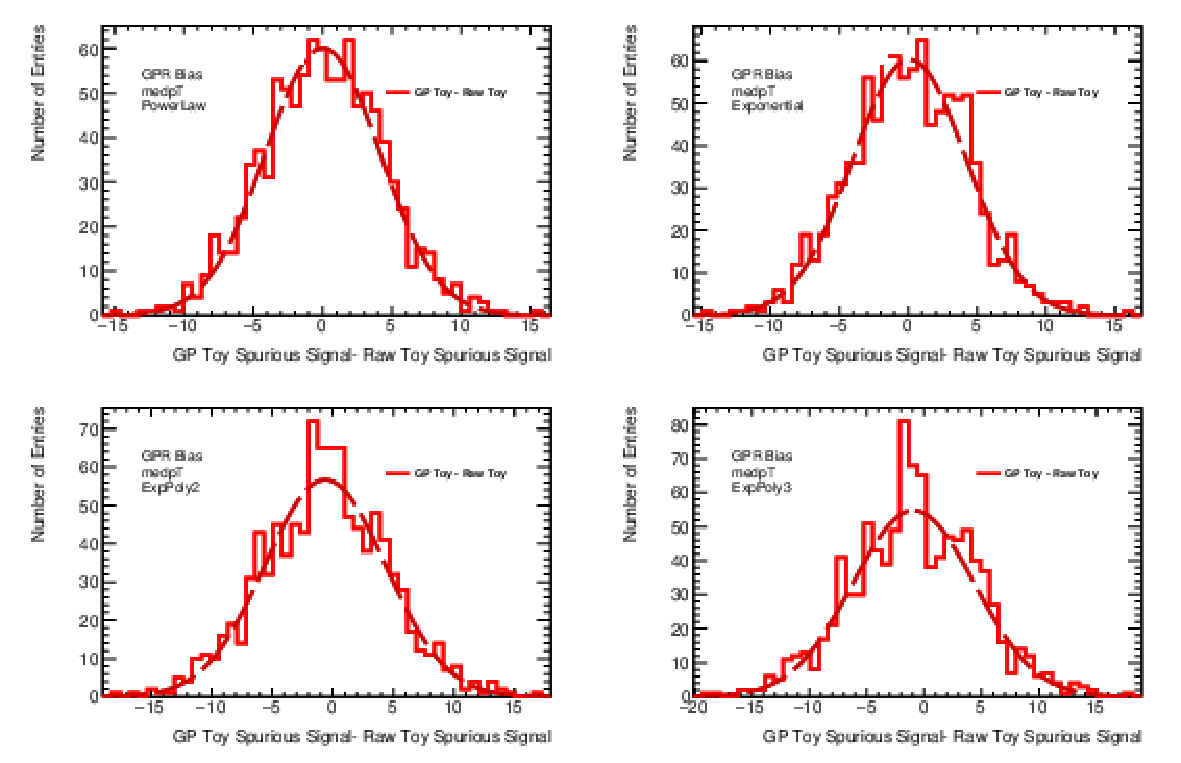
\includegraphics[width=\textwidth]{figures/background/gpr/validation/nominal/ToyTest_FitSigBiases_medpT_100k_noSig}   
\caption{The per-toy bias (GP Spurious Signal - Raw Spurious Signal), using an expPoly3-derived template. Each toy in this test has 100k events.}
\label{fig:bias_medpt_100k_noSig}
\end{center}
\end{figure}

\begin{figure} 
\begin{center}
  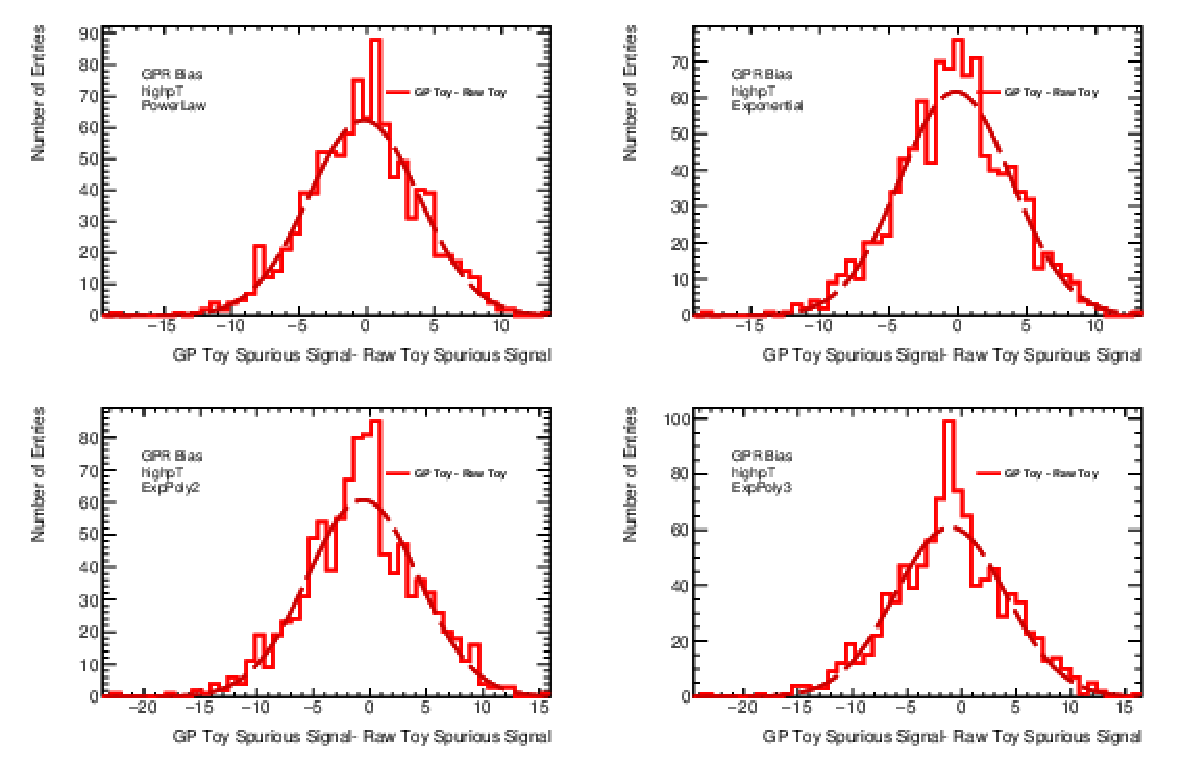
\includegraphics[width=\textwidth]{figures/background/gpr/validation/nominal/ToyTest_FitSigBiases_highpT_100k_noSig}   
\caption{The per-toy bias (GP Spurious Signal - Raw Spurious Signal), using a different expPoly3-derived template. Each toy in this test has 100k events.}
\label{fig:bias_highpt_100k_noSig}
\end{center}
\end{figure}

\begin{figure} 
\begin{center}
  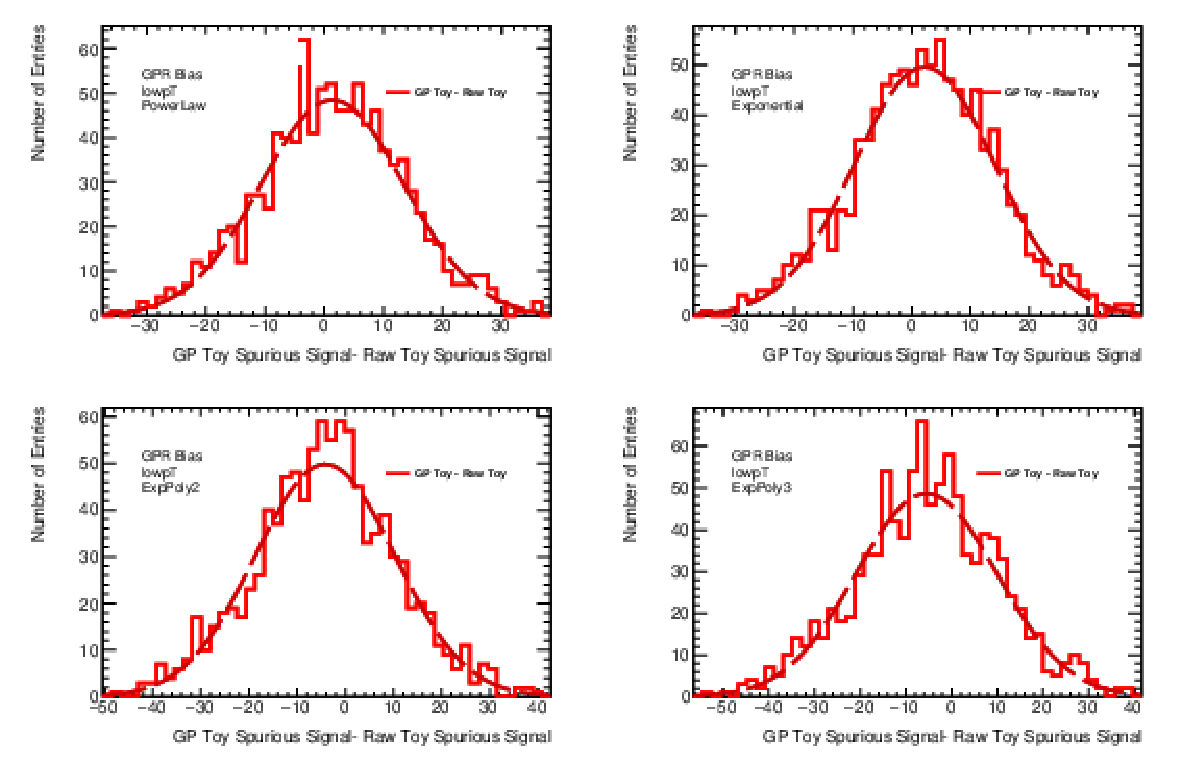
\includegraphics[width=\textwidth]{figures/background/gpr/validation/nominal/ToyTest_FitSigBiases_lowpT_1M_noSig}   
\caption{The per-toy bias (GP Spurious Signal - Raw Spurious Signal), using an expPoly2-derived template. Each toy in this test has 1,000,000 events.}
\label{fig:bias_lowpt_1M_noSig}
\end{center}
\end{figure}

\begin{figure} 
\begin{center}
  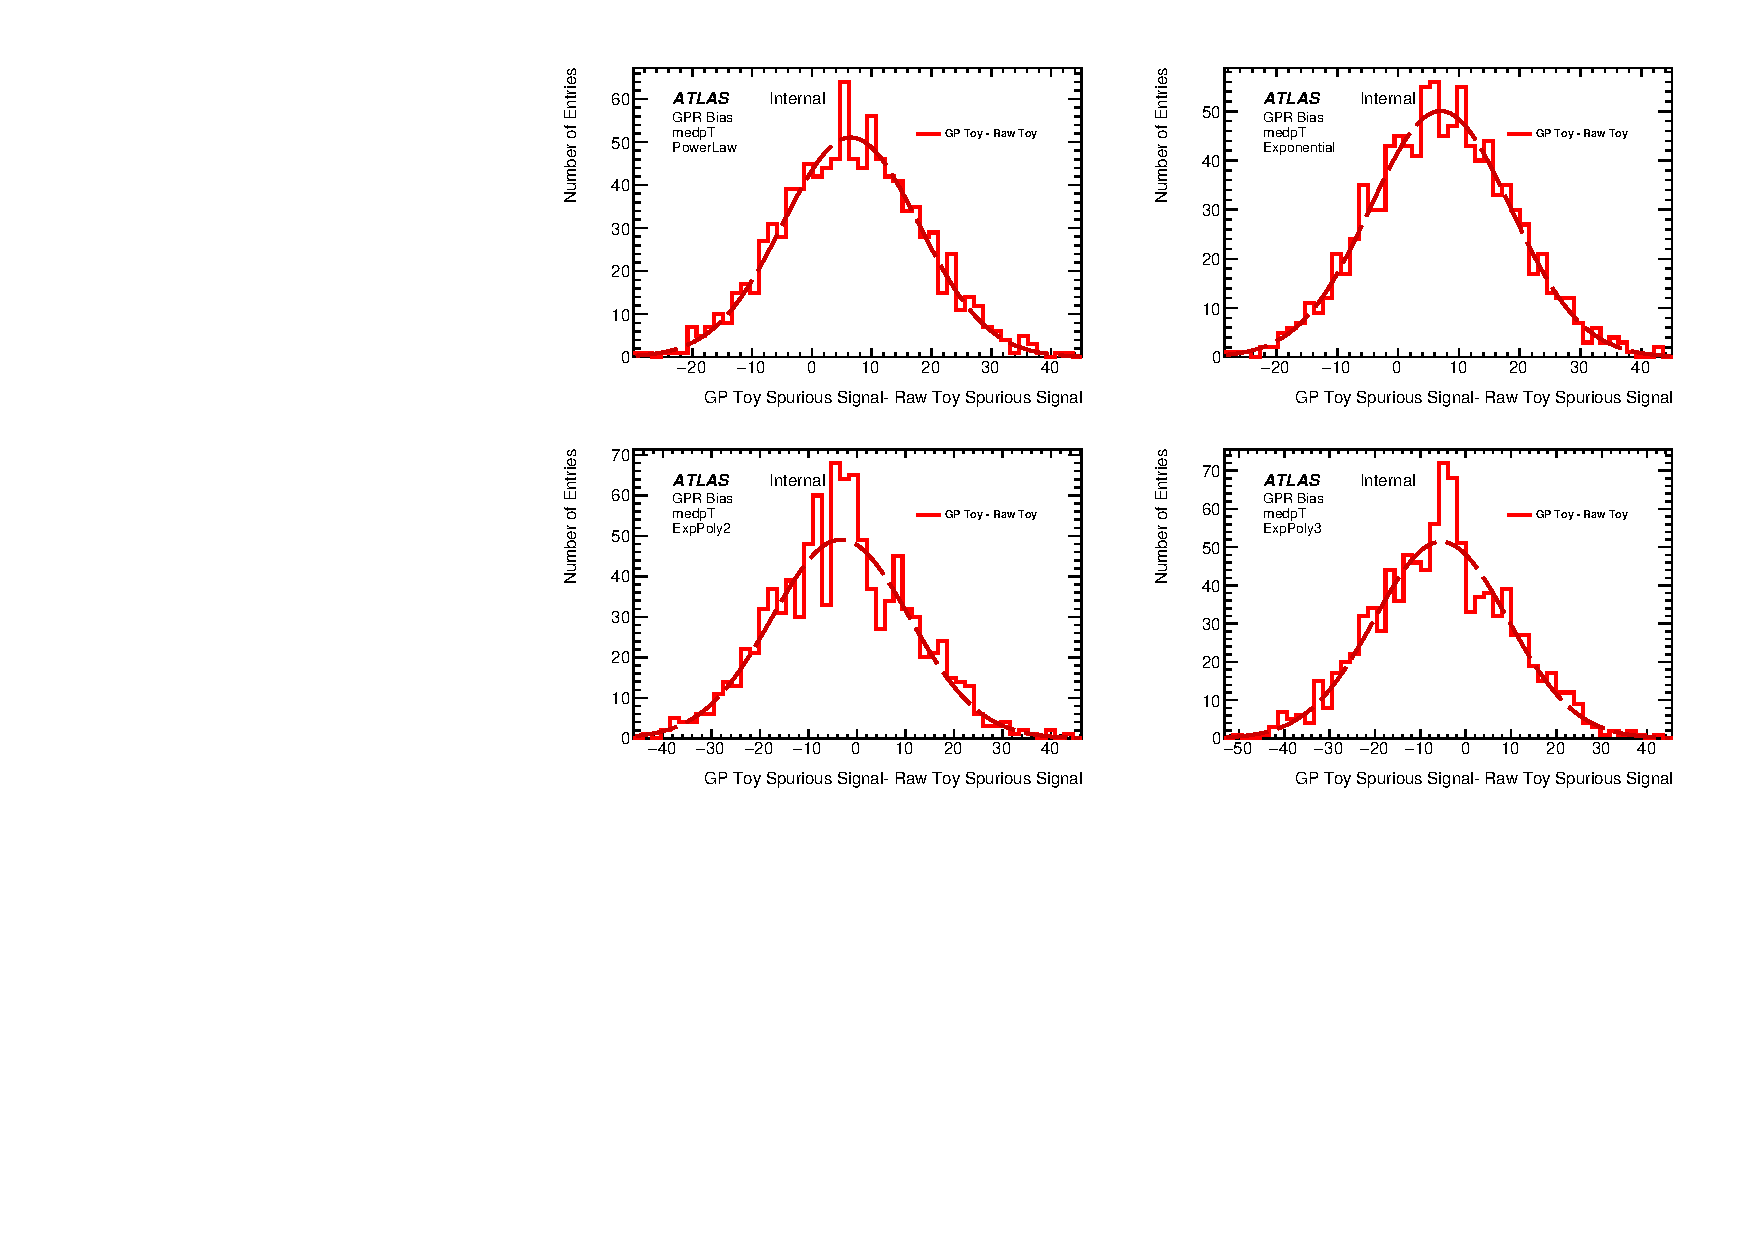
\includegraphics[width=\textwidth]{figures/background/gpr/validation/nominal/ToyTest_FitSigBiases_medpT_1M_noSig}   
\caption{The per-toy bias (GP Spurious Signal - Raw Spurious Signal), using an expPoly3-derived template. Each toy in this test has 1,000,000 events.}
\label{fig:bias_medpt_1M_noSig}
\end{center}
\end{figure}

\begin{figure} 
\begin{center}
  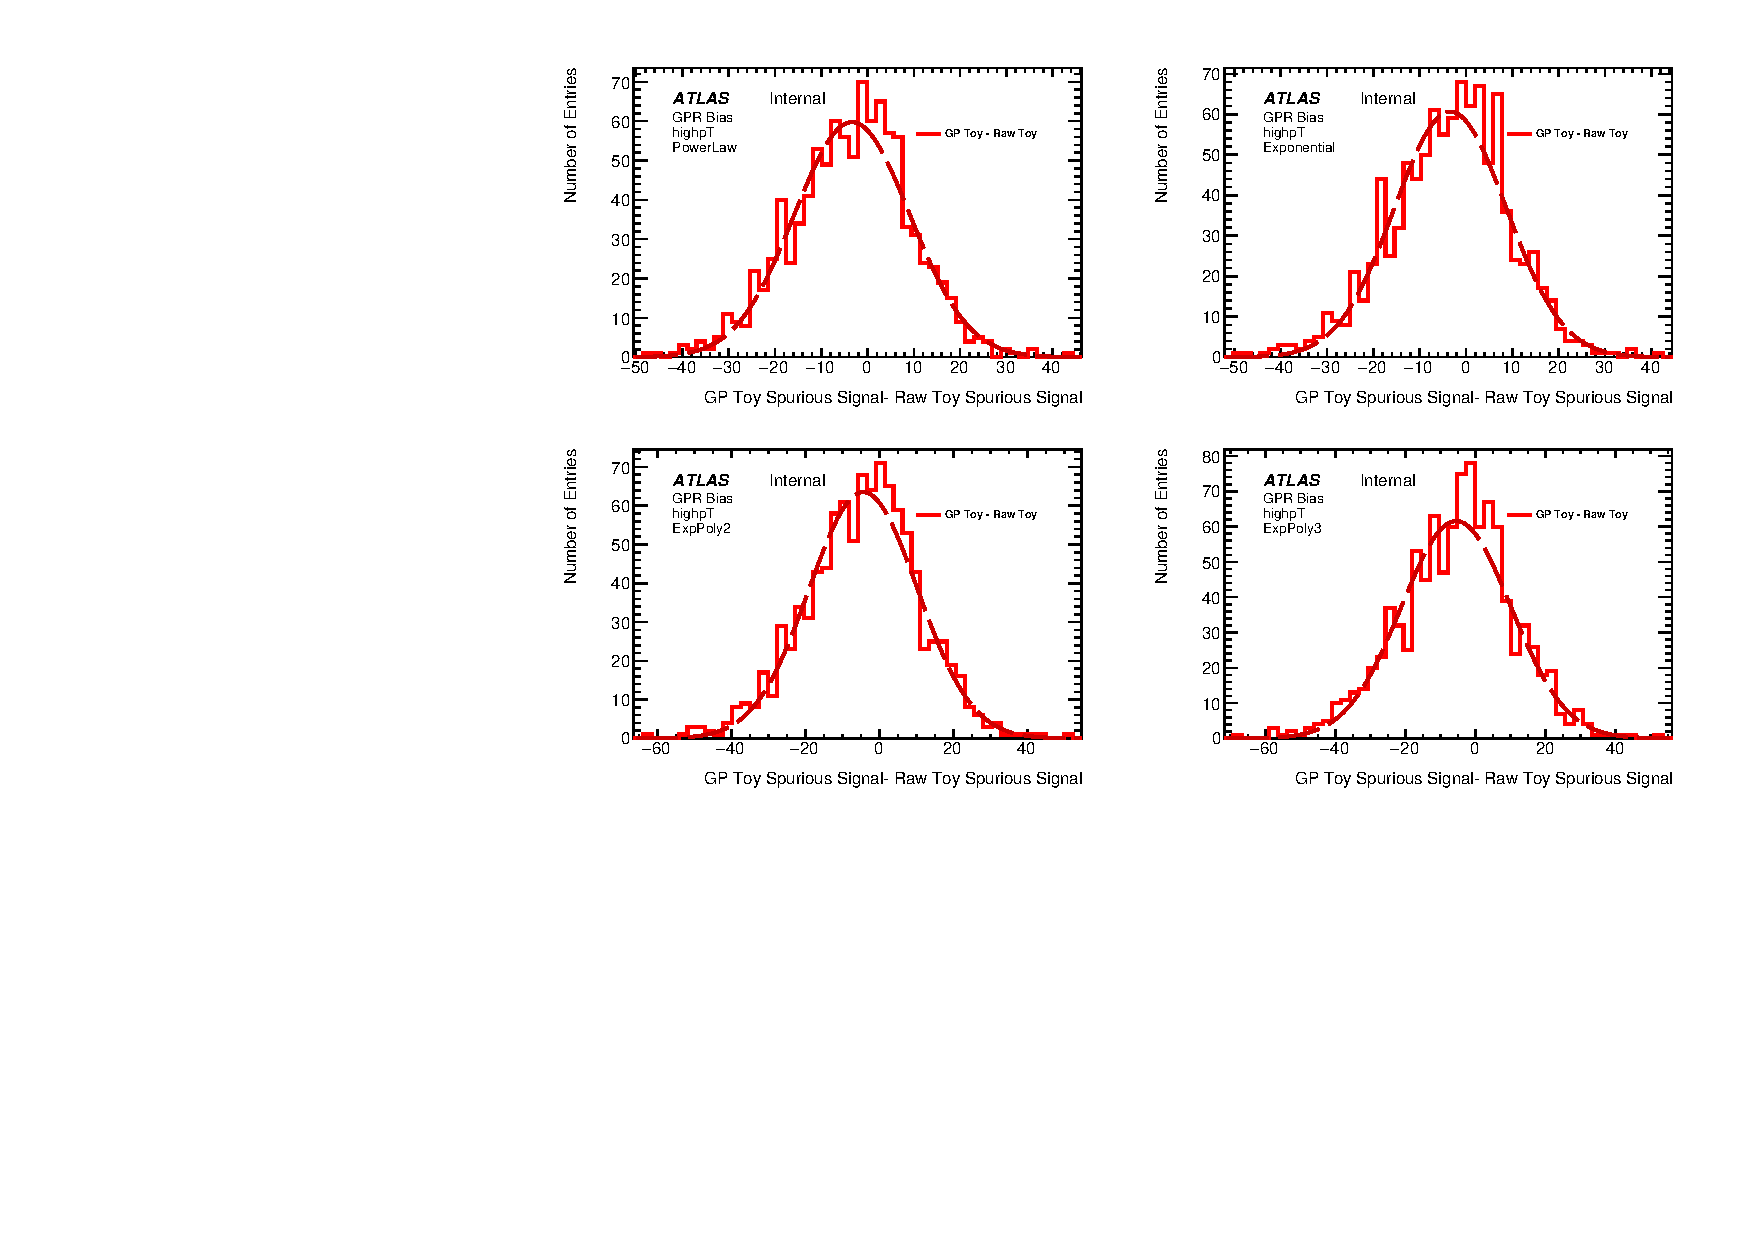
\includegraphics[width=\textwidth]{figures/background/gpr/validation/nominal/ToyTest_FitSigBiases_highpT_1M_noSig}   
\caption{The per-toy bias (GP Spurious Signal - Raw Spurious Signal), using a different expPoly3-derived template. Each toy in this test has 1,000,000 events.}
\label{fig:bias_highpt_1M_noSig}
\end{center}
\end{figure}

\begin{figure} 
\begin{center}
  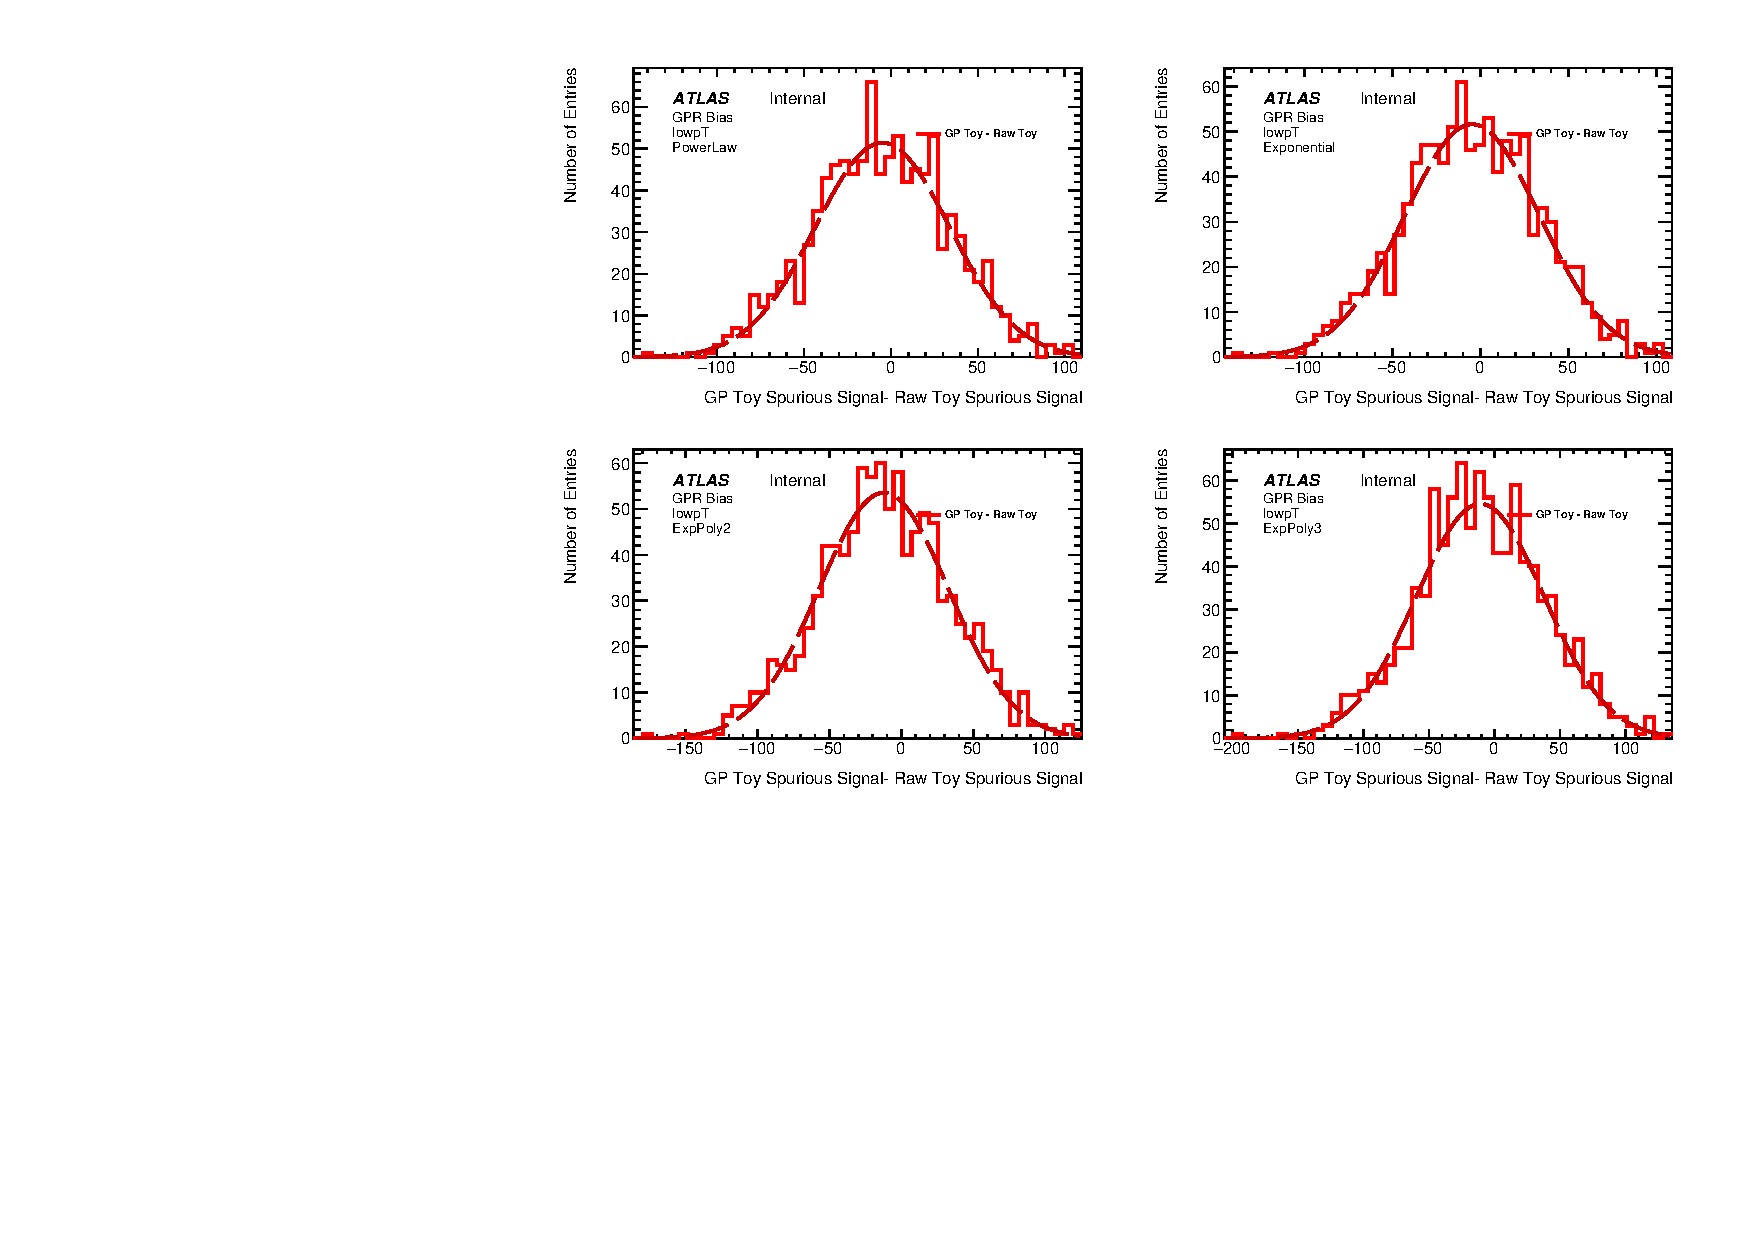
\includegraphics[width=\textwidth]{figures/background/gpr/validation/nominal/ToyTest_FitSigBiases_lowpT_10M_noSig}   
\caption{The per-toy bias (GP Spurious Signal - Raw Spurious Signal), using an expPoly2-derived template. Each toy in this test has 10,000,000 events.}
\label{fig:bias_lowpt_10M_noSig}
\end{center}
\end{figure}

\begin{figure} 
\begin{center}
  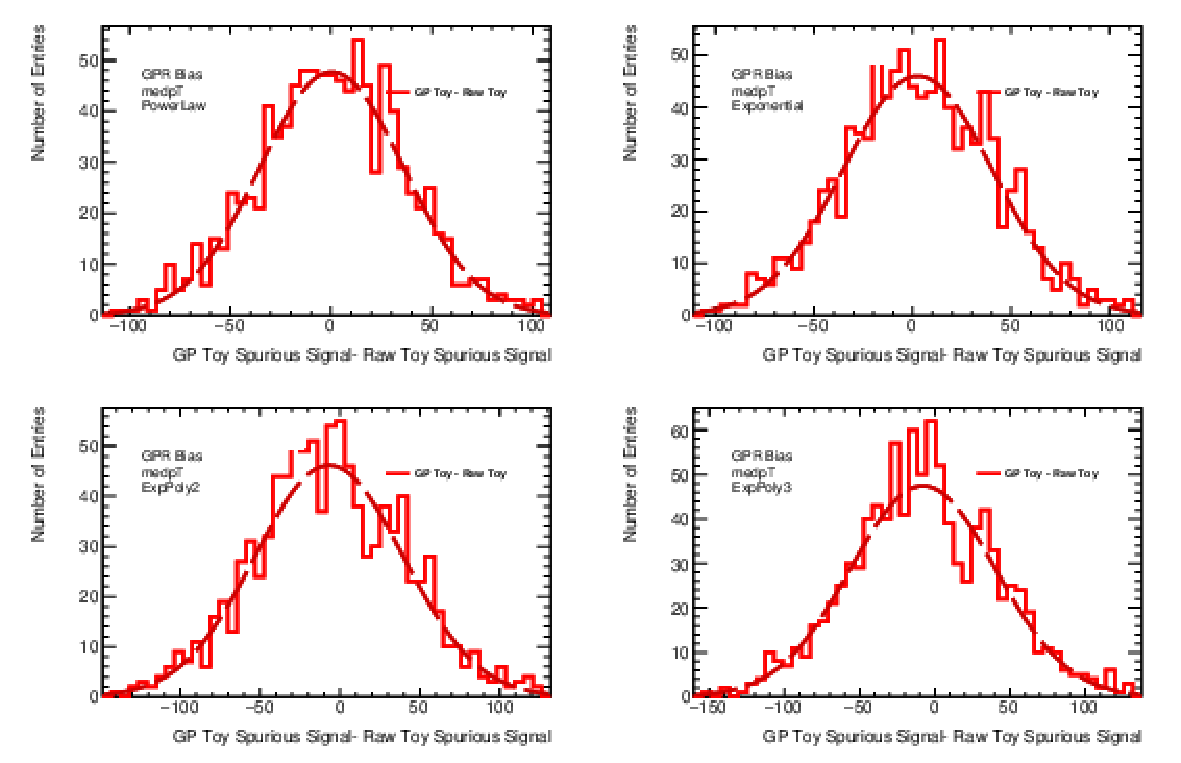
\includegraphics[width=\textwidth]{figures/background/gpr/validation/nominal/ToyTest_FitSigBiases_medpT_10M_noSig}   
\caption{The per-toy bias (GP Spurious Signal - Raw Spurious Signal), using an expPoly3-derived template. Each toy in this test has 10,000,000 events.}
\label{fig:bias_medpt_10M_noSig}
\end{center}
\end{figure}

\begin{figure} 
\begin{center}
  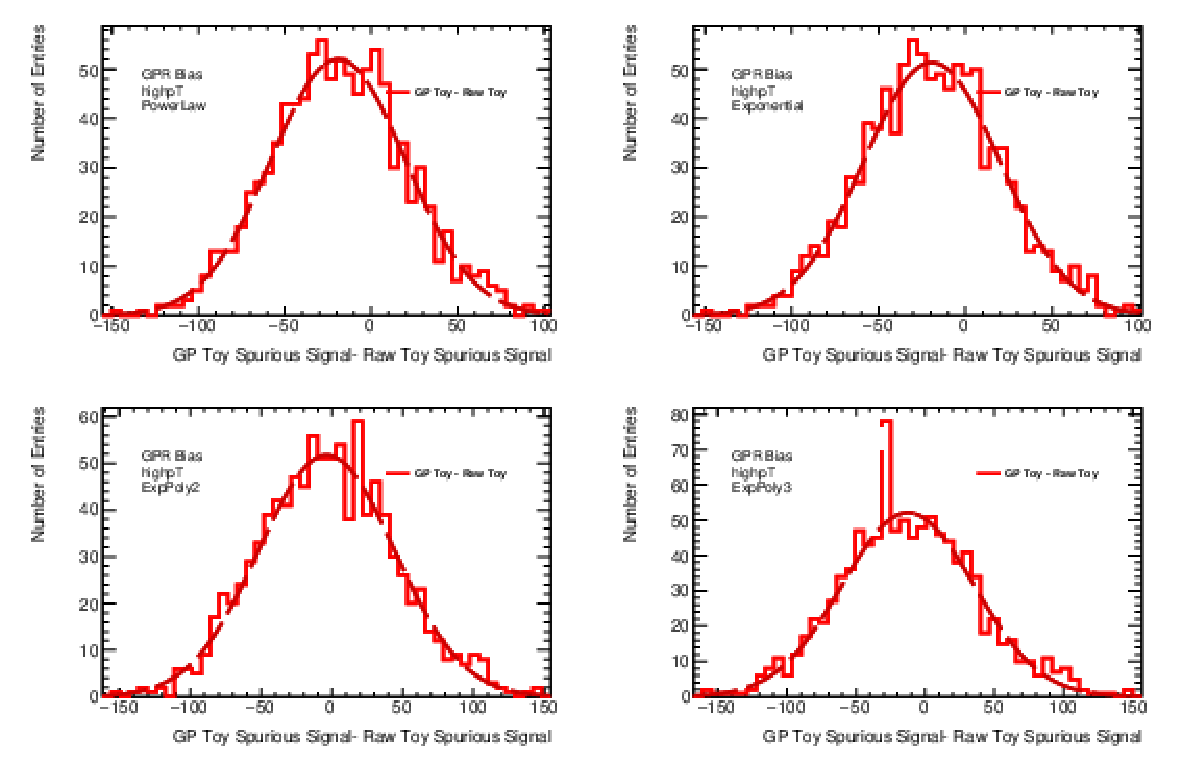
\includegraphics[width=\textwidth]{figures/background/gpr/validation/nominal/ToyTest_FitSigBiases_highpT_10M_noSig}   
\caption{The per-toy bias (GP Spurious Signal - Raw Spurious Signal), using a different expPoly3-derived template. Each toy in this test has 10,000,000 events.}
\label{fig:bias_highpt_10M_noSig}
\end{center}
\end{figure}

To determine how to reduce the bias further, we note a further set of tests performed in an earlier iteration of this method \cite{Hyneman}, evaluating the difference in GP fit bias when different functional priors were used as the GP mean. The Exponential function, Linear function, and a flat line were all tested. These tests were performed using templates constructed from Power Law (Fig.~\ref{fig:prior_bias_powerlaw}), ExpPoly2 (Fig.~\ref{fig:prior_bias_exppoly2}), and Bernstein 5 (Fig.~\ref{fig:prior_bias_bern5}) functions. Again, different levels of statistics in the templates were tested. Overall, the choice of GP mean does not seem to affect the GP fit behavior significantly, other than for templates with less than 10 effective MC events per bin. The unit of the y-axis in these plots is the percentage disagreement between the smoothed and the unsmoothed template, similar to a ratio plot.

In the lower statistics templates, most of the differences in fitting bias are again confined to the extremities of the template range, as expected, and can be reduced by padding the template with dummy bins. Furthermore, the use of the $\chi^2$ method to automatically select the flat prior in lower-statistics regions means that, in regions where the choice of prior matters, we are automatically choosing the one that best fits the data. Thus, the choice of prior does not appear to introduce a significant bias in the fit result. 

\begin{figure} 
\begin{center}
  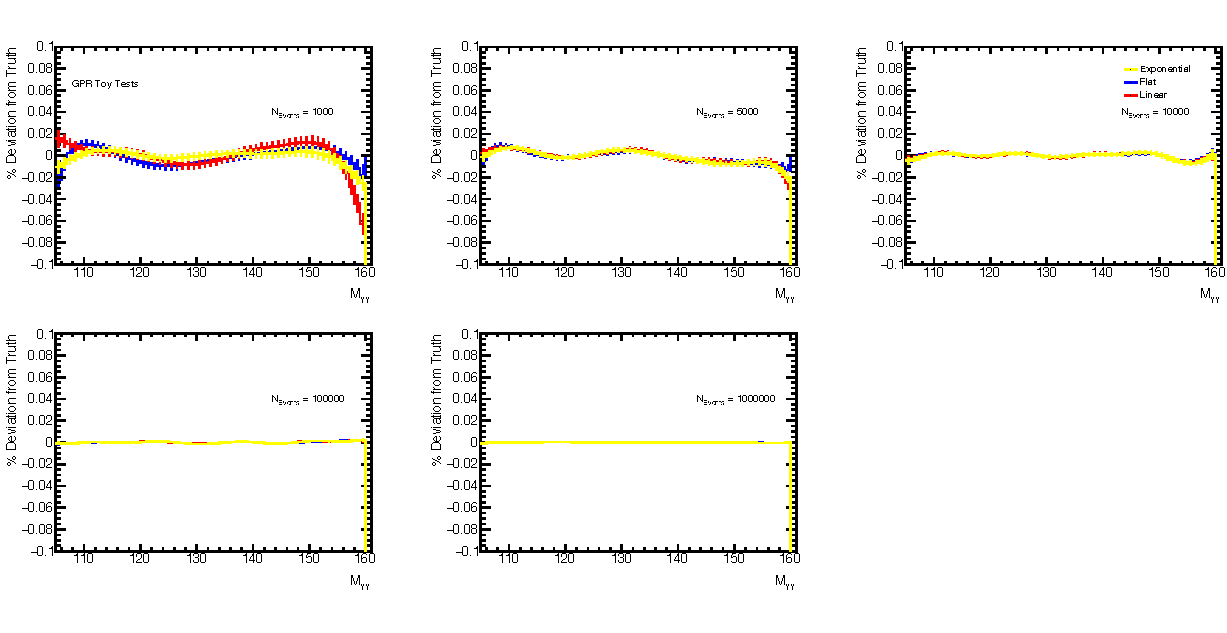
\includegraphics[width=\textwidth]{figures/background/gpr/checkBiasFromPriorChoice/Plots_GPR_PriorBiases_PowerLaw_crop}   
  \caption{Comparisons of the average bias induced by the choice of GP mean when fitting toy templates constructed from the analytic Power Law function. The yellow shape shows the results using the default Exponential mean, the blue shape shows the result using a flat line as the mean, and the red shape shows the result using a linear fit as the mean. The top left subplot shows the results using templates containing 1000 events, the top middle shows the results using templates containing 5000 events, and the top right shows the results using templates containing 10,000 events. The bottom left subplot shows the results using templates containing 100,000 events, while the bottom middle shows the results using templates containing one million events.}
\label{fig:prior_bias_powerlaw}
\end{center}
\end{figure}

\begin{figure} 
\begin{center}
  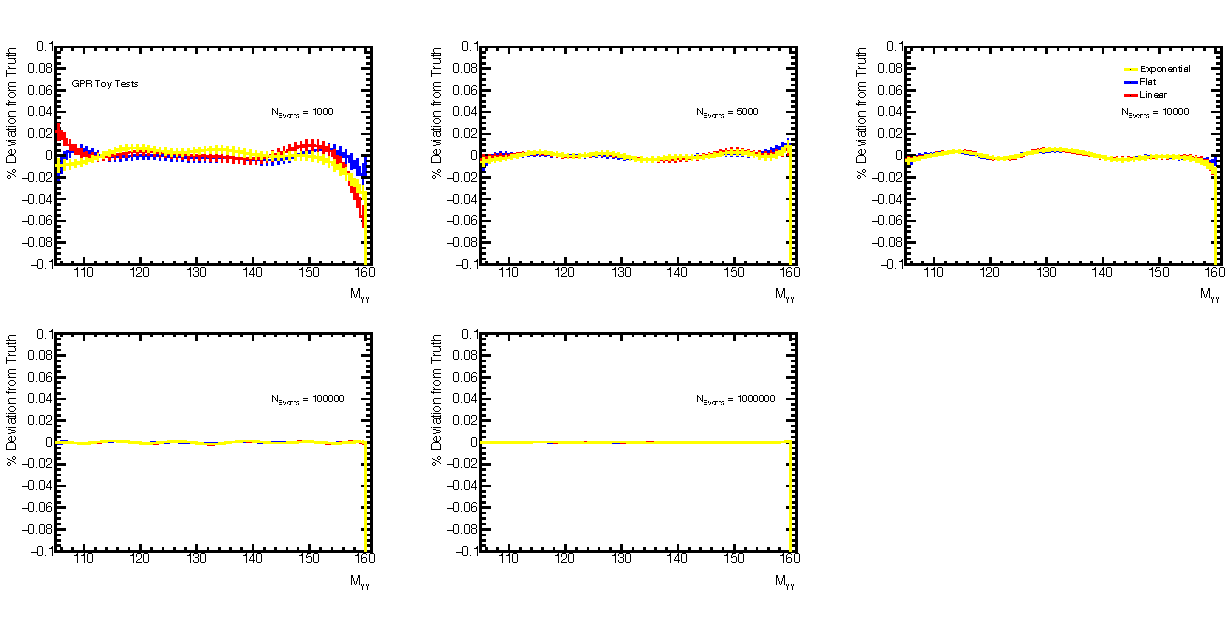
\includegraphics[width=\textwidth]{figures/background/gpr/checkBiasFromPriorChoice/Plots_GPR_PriorBiases_ExpPoly2_crop}   
   \caption{Comparisons of the average bias induced by the choice of GP mean when fitting toy templates constructed from the analytic ExpPoly2 function. The yellow shape shows the results using the default Exponential mean, the blue shape shows the result using a flat line as the mean, and the red shape shows the result using a linear fit as the mean. The top left subplot shows the results using templates containing 1000 events, the top middle shows the results using templates containing 5000 events, and the top right shows the results using templates containing 10,000 events. The bottom left subplot shows the results using templates containing 100,000 events, while the bottom middle shows the results using templates containing one million events.}
\label{fig:prior_bias_exppoly2}
\end{center}
\end{figure}

\begin{figure} 
\begin{center}
  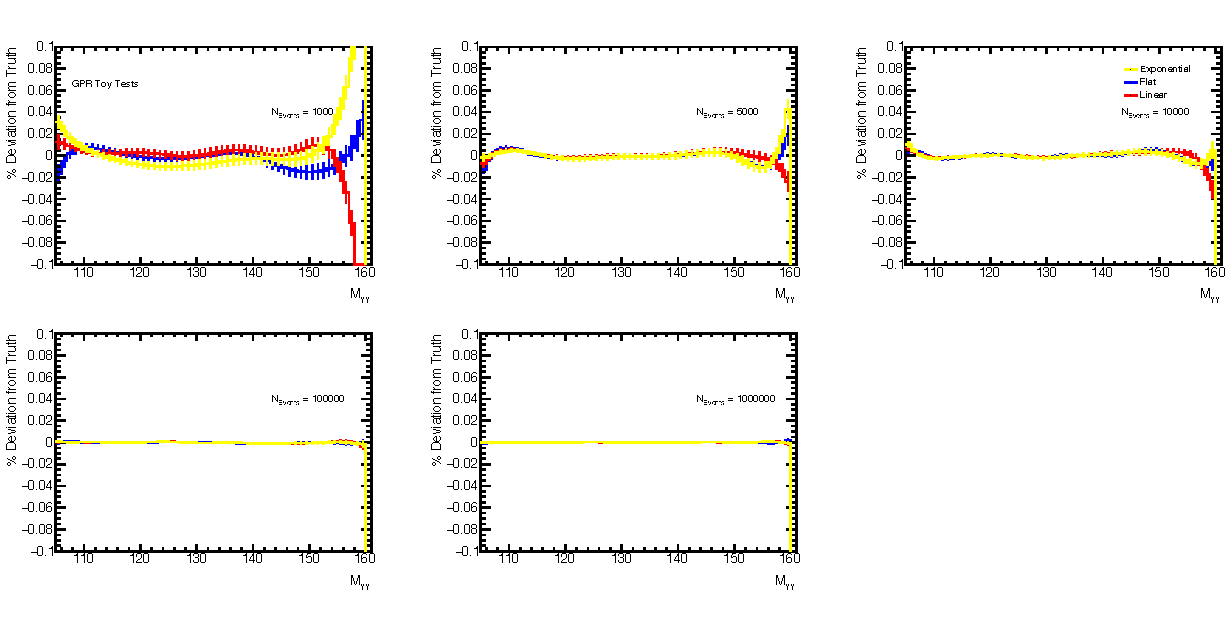
\includegraphics[width=\textwidth]{figures/background/gpr/checkBiasFromPriorChoice/Plots_GPR_PriorBiases_Bern5_crop}   
   \caption{Comparisons of the average bias induced by the choice of GP mean when fitting toy templates constructed from the analytic Bernstein 5 function. The yellow shape shows the results using the default Exponential mean, the blue shape shows the result using a flat line as the mean, and the red shape shows the result using a linear fit as the mean. The top left subplot shows the results using templates containing 1000 events, the top middle shows the results using templates containing 5000 events, and the top right shows the results using templates containing 10,000 events. The bottom left subplot shows the results using templates containing 100,000 events, while the bottom middle shows the results using templates containing one million events.}
\label{fig:prior_bias_bern5}
\end{center}
\end{figure}

\subsection{Extended Templates}

Some disagreement between the nominal template and the GP template is observed at the edges of the plots. To reduce this, larger templates can be provided to the GP- that is, we perform the GP fit on templates in the mass range 100-165 GeV, but perform the spurious signal test on the smoothed and unsmoothed template in the range 105-160 GeV, thus relegating the edge effects to the outer 5 bins. We show that extending the templates in this manner reduces the bias observed from 40\% to 25\% of the statistical uncertainty on the spurious signal.

To approximate this extension, we can also perform a linear fit padding on the templates, extending the templates by 5 bins on either side based on the slope of the first and last 5 bins. 
\begin{figure} 
\begin{center}
  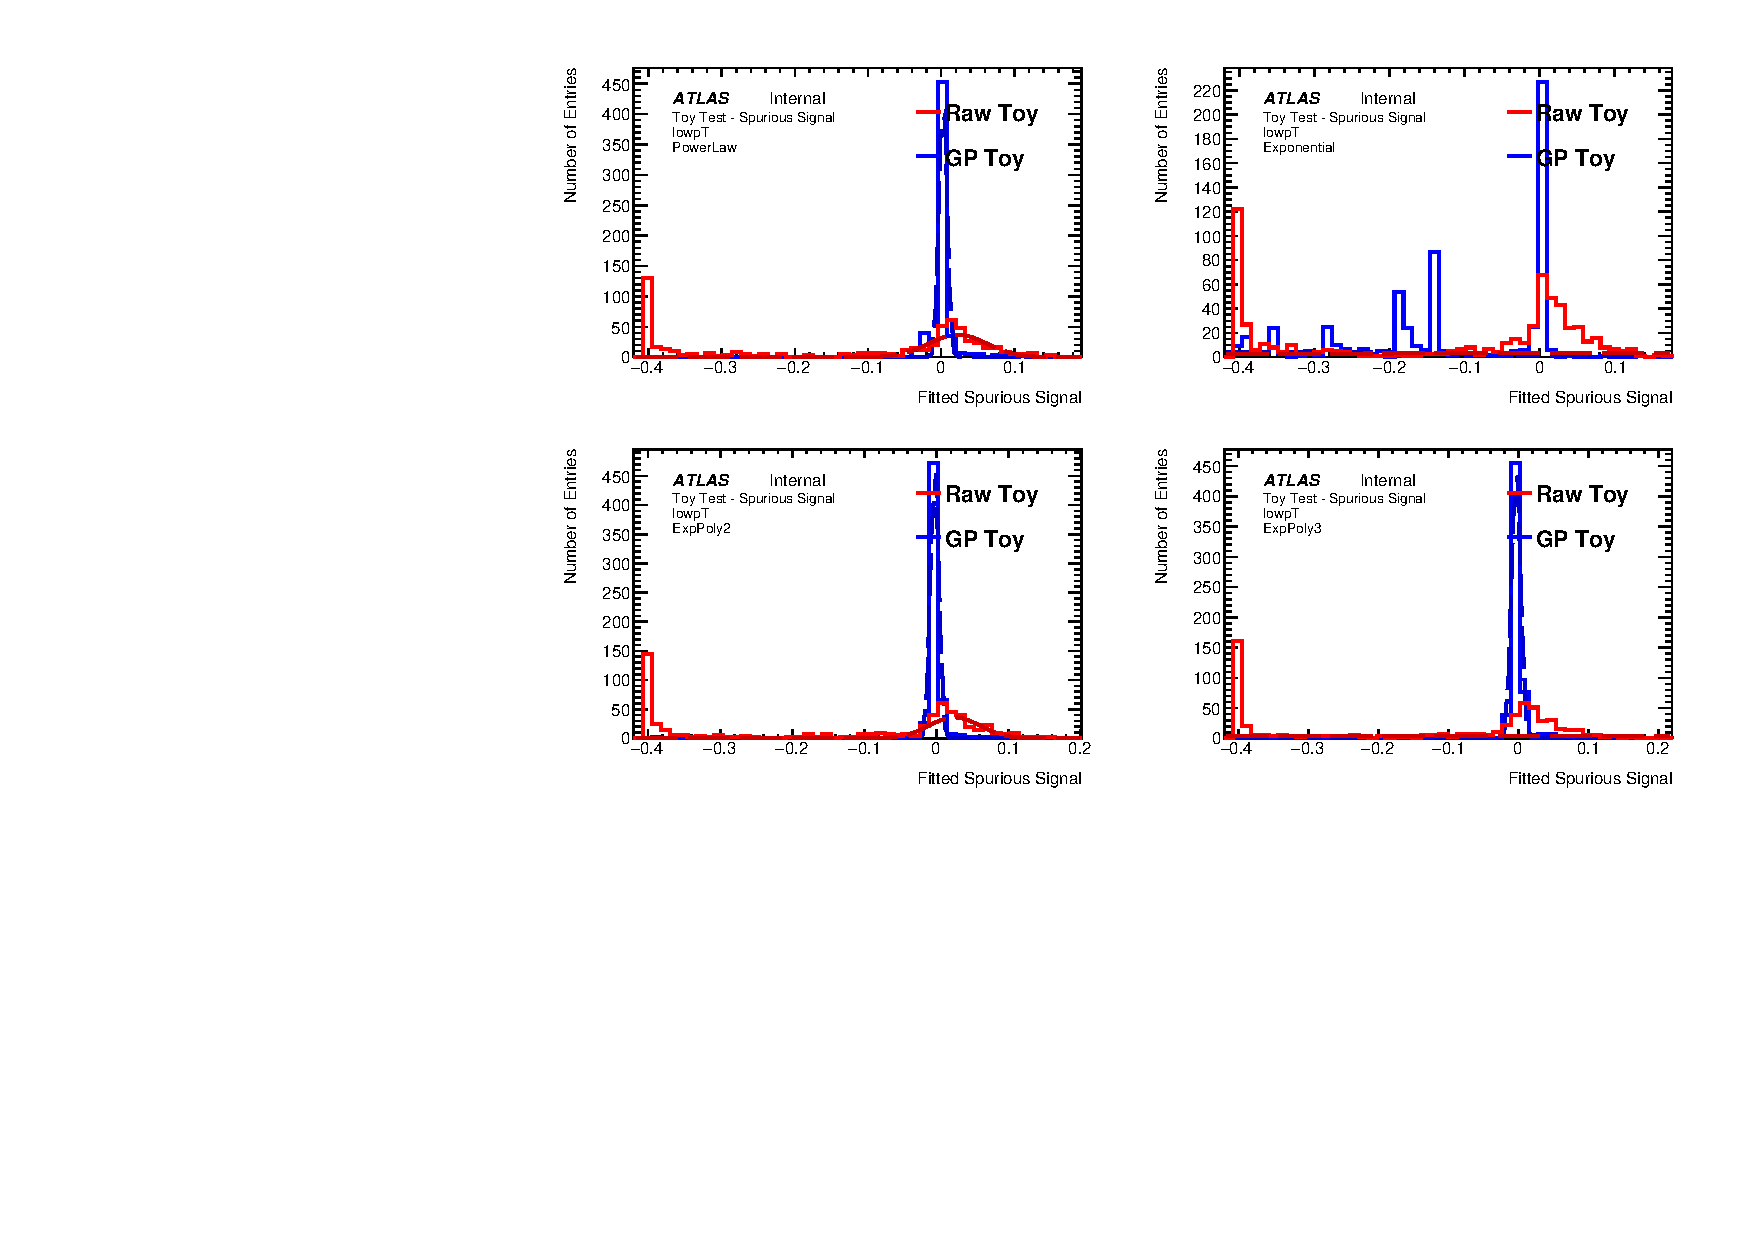
\includegraphics[width=\textwidth]{figures/background/gpr/validation/padded/ToyTest_FitSigVals_lowpT_10_noSig}   
\caption{The distribution of spurious signal for various functions for both the GPR and raw template, using an expPoly2-derived template extended by 5 bins on either side. Each toy in this test has 10 events.}
\label{fig:padded_lowpt_10_noSig}
\end{center}
\end{figure}

\begin{figure} 
\begin{center}
  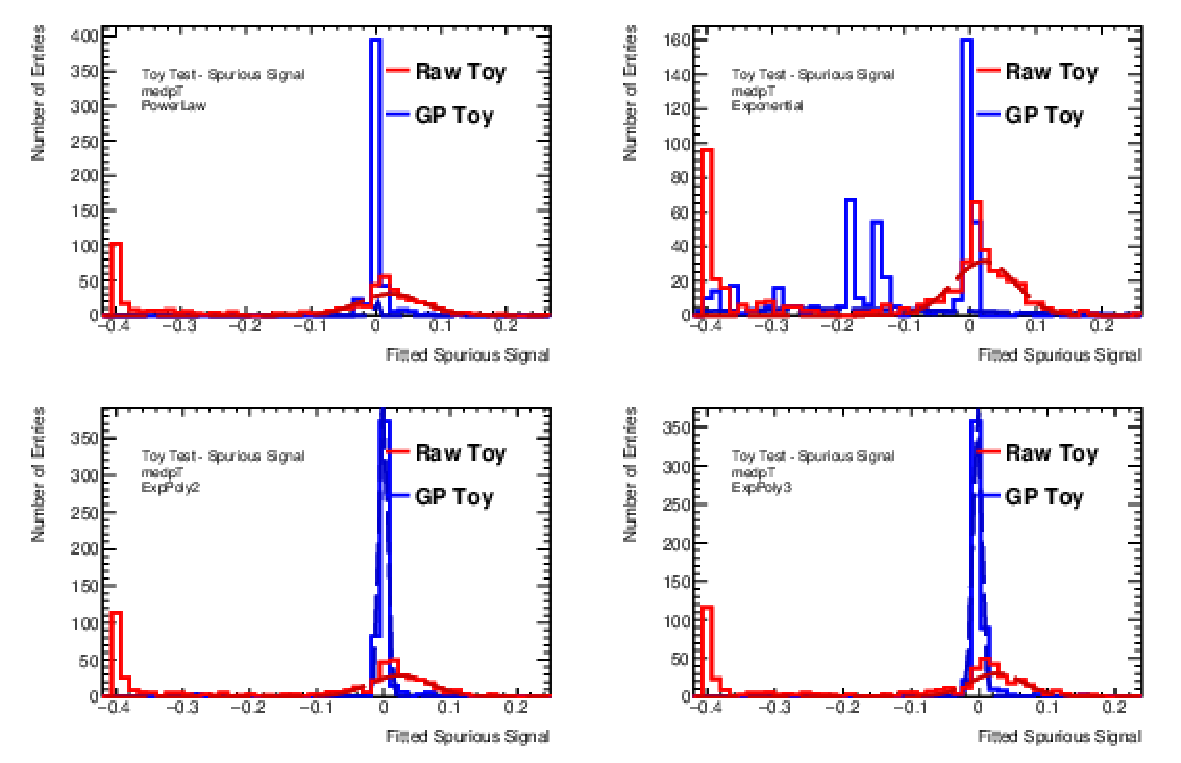
\includegraphics[width=\textwidth]{figures/background/gpr/validation/padded/ToyTest_FitSigVals_medpT_10_noSig}   
\caption{The distribution of spurious signal for various functions for both the GPR and raw template, using an expPoly3-derived template extended by 5 GeV on either side. Each toy in this test has 10 events.}
\label{fig:padded_medpt_10_noSig}
\end{center}
\end{figure}

\begin{figure} 
\begin{center}
  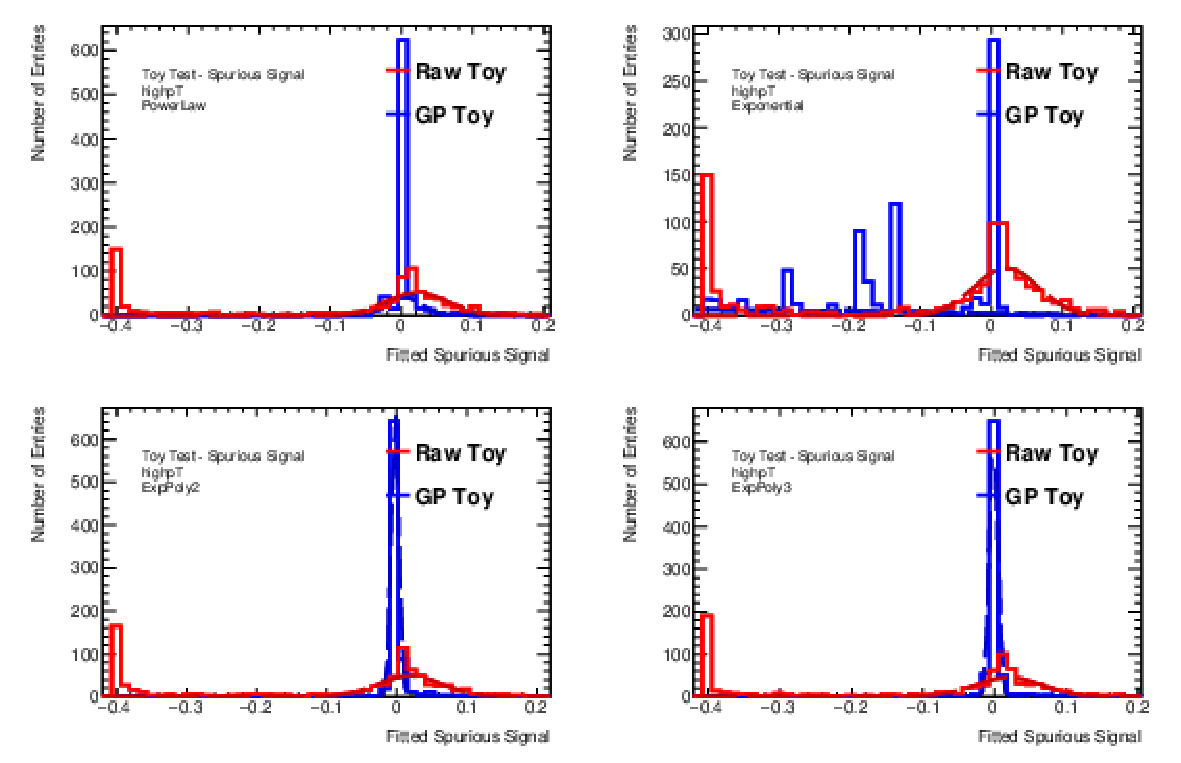
\includegraphics[width=\textwidth]{figures/background/gpr/validation/padded/ToyTest_FitSigVals_highpT_10_noSig}   
\caption{The distribution of spurious signal for various functions for both the GPR and raw template, using a different expPoly3-derived template extended by 5 GeV on either side. Each toy in this test has 10 events.}
\label{fig:padded_highpt_10_noSig}
\end{center}
\end{figure}

\begin{figure} 
\begin{center}
  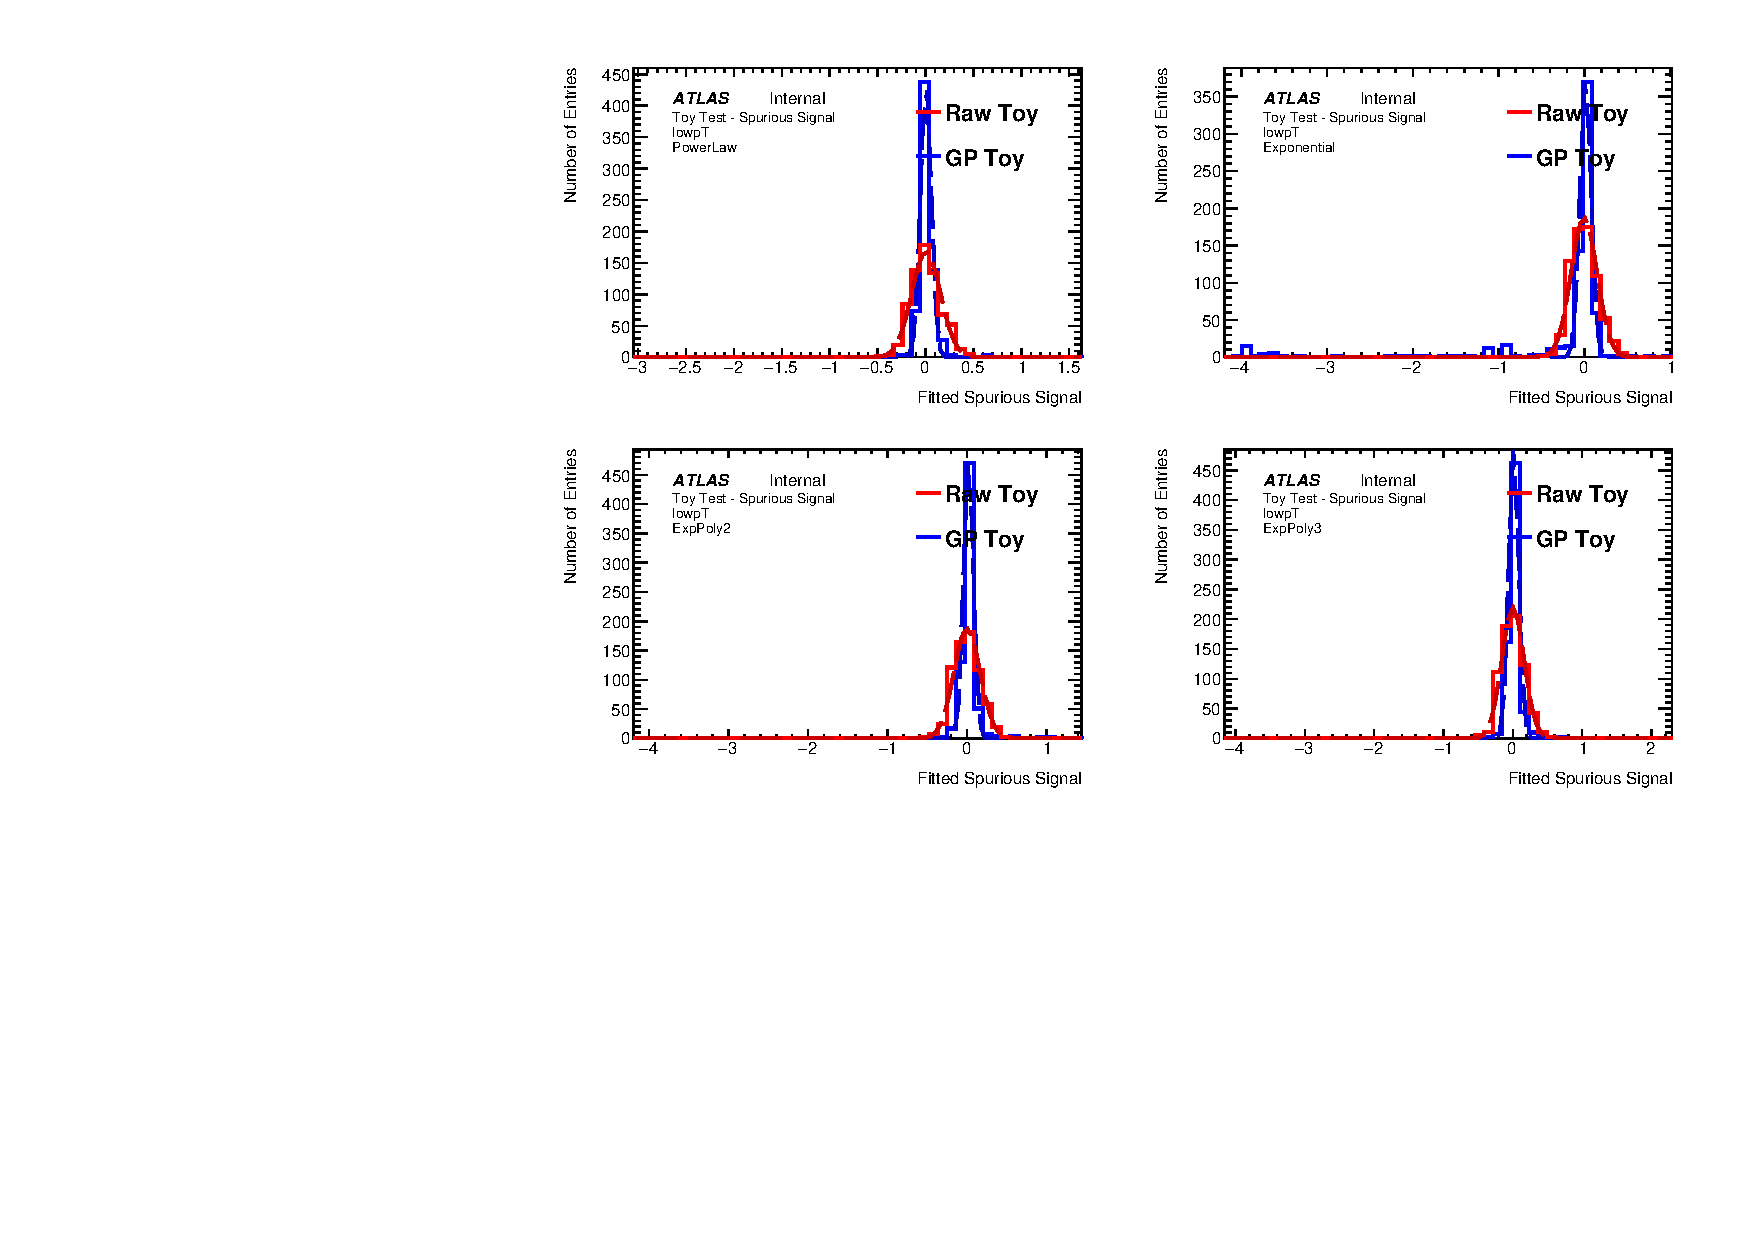
\includegraphics[width=\textwidth]{figures/background/gpr/validation/padded/ToyTest_FitSigVals_lowpT_100_noSig}   
\caption{The distribution of spurious signal for various functions for both the GPR and raw template, using an expPoly2-derived template extended by 5 GeV on either side. Each toy in this test has 100 events.}
\label{fig:padded_lowpt_100_noSig}
\end{center}
\end{figure}

\begin{figure} 
\begin{center}
  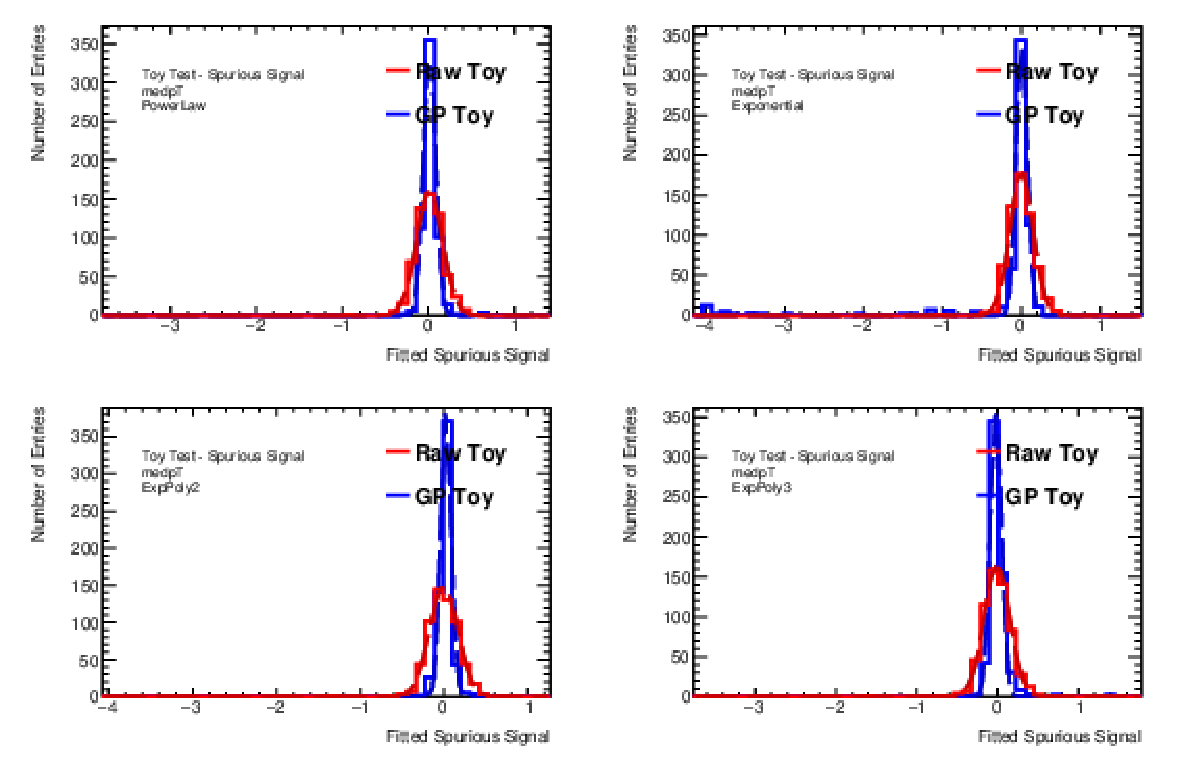
\includegraphics[width=\textwidth]{figures/background/gpr/validation/padded/ToyTest_FitSigVals_medpT_100_noSig}   
\caption{The distribution of spurious signal for various functions for both the GPR and raw template, using an expPoly3-derived template extended by 5 GeV on either side. Each toy in this test has 100 events.}
\label{fig:padded_medpt_100_noSig}
\end{center}
\end{figure}

\begin{figure} 
\begin{center}
  \includegraphics[width=\textwidth]{figures/background/gpr/validation/padded/ToyTest_FitSigVals_highpT_100_noSig}   
\caption{The distribution of spurious signal for various functions for both the GPR and raw template, using a different expPoly3-derived template extended by 5 GeV on either side. Each toy in this test has 100 events.}
\label{fig:padded_highpt_100_noSig}
\end{center}
\end{figure}

\begin{figure} 
\begin{center}
  \includegraphics[width=\textwidth]{figures/background/gpr/validation/padded/ToyTest_FitSigVals_lowpT_1000_noSig}   
\caption{The distribution of spurious signal for various functions for both the GPR and raw template, using an expPoly2-derived template extended by 5 GeV on either side. Each toy in this test has 1000 events.}
\label{fig:padded_lowpt_1000_noSig}
\end{center}
\end{figure}

\begin{figure} 
\begin{center}
  \includegraphics[width=\textwidth]{figures/background/gpr/validation/padded/ToyTest_FitSigVals_medpT_1000_noSig}   
\caption{The distribution of spurious signal for various functions for both the GPR and raw template, using an expPoly3-derived template extended by 5 GeV on either side. Each toy in this test has 1000 events.}
\label{fig:padded_medpt_1000_noSig}
\end{center}
\end{figure}

\begin{figure} 
\begin{center}
  \includegraphics[width=\textwidth]{figures/background/gpr/validation/padded/ToyTest_FitSigVals_highpT_1000_noSig}   
\caption{The distribution of spurious signal for various functions for both the GPR and raw template, using a different expPoly3-derived template extended by 5 GeV on either side. Each toy in this test has 1000 events.}
\label{fig:padded_highpt_1000_noSig}
\end{center}
\end{figure}

\begin{figure} 
\begin{center}
  \includegraphics[width=\textwidth]{figures/background/gpr/validation/padded/ToyTest_FitSigVals_lowpT_10k_noSig}   
\caption{The distribution of spurious signal for various functions for both the GPR and raw template, using an expPoly2-derived template extended by 5 GeV on either side. Each toy in this test has 10k events.}
\label{fig:padded_lowpt_10k_noSig}
\end{center}
\end{figure}

\begin{figure} 
\begin{center}
  \includegraphics[width=\textwidth]{figures/background/gpr/validation/padded/ToyTest_FitSigVals_medpT_10k_noSig}   
\caption{The distribution of spurious signal for various functions for both the GPR and raw template, using an expPoly3-derived template extended by 5 GeV on either side. Each toy in this test has 10k events.}
\label{fig:padded_medpt_10k_noSig}
\end{center}
\end{figure}

\begin{figure} 
\begin{center}
  \includegraphics[width=\textwidth]{figures/background/gpr/validation/padded/ToyTest_FitSigVals_highpT_10k_noSig}   
\caption{The distribution of spurious signal for various functions for both the GPR and raw template, using a different expPoly3-derived template extended by 5 GeV on either side. Each toy in this test has 10k events.}
\label{fig:padded_highpt_10k_noSig}
\end{center}
\end{figure}

\begin{figure} 
\begin{center}
  \includegraphics[width=\textwidth]{figures/background/gpr/validation/padded/ToyTest_FitSigVals_lowpT_100k_noSig}   
\caption{The distribution of spurious signal for various functions for both the GPR and raw template, using an expPoly2-derived template extended by 5 GeV on either side. Each toy in this test has 100k events.}
\label{fig:padded_lowpt_100k_noSig}
\end{center}
\end{figure}

\begin{figure} 
\begin{center}
  \includegraphics[width=\textwidth]{figures/background/gpr/validation/padded/ToyTest_FitSigVals_medpT_100k_noSig}   
\caption{The distribution of spurious signal for various functions for both the GPR and raw template, using an expPoly3-derived template extended by 5 GeV on either side. Each toy in this test has 100k events.}
\label{fig:padded_medpt_100k_noSig}
\end{center}
\end{figure}

\begin{figure} 
\begin{center}
  \includegraphics[width=\textwidth]{figures/background/gpr/validation/padded/ToyTest_FitSigVals_highpT_100k_noSig}   
\caption{The distribution of spurious signal for various functions for both the GPR and raw template, using a different expPoly3-derived template extended by 5 GeV on either side. Each toy in this test has 100k events.}
\label{fig:padded_highpt_100k_noSig}
\end{center}
\end{figure}

\begin{figure} 
\begin{center}
  \includegraphics[width=\textwidth]{figures/background/gpr/validation/padded/ToyTest_FitSigVals_lowpT_1M_noSig}   
\caption{The distribution of spurious signal for various functions for both the GPR and raw template, using an expPoly2-derived template extended by 5 GeV on either side. Each toy in this test has 1,000,000 events.}
\label{fig:padded_lowpt_1M_noSig}
\end{center}
\end{figure}

\begin{figure} 
\begin{center}
  \includegraphics[width=\textwidth]{figures/background/gpr/validation/padded/ToyTest_FitSigVals_medpT_1M_noSig}   
\caption{The distribution of spurious signal for various functions for both the GPR and raw template, using an expPoly3-derived template extended by 5 GeV on either side. Each toy in this test has 1,000,000 events.}
\label{fig:padded_medpt_1M_noSig}
\end{center}
\end{figure}

\begin{figure} 
\begin{center}
  \includegraphics[width=\textwidth]{figures/background/gpr/validation/padded/ToyTest_FitSigVals_highpT_1M_noSig}   
\caption{The distribution of spurious signal for various functions for both the GPR and raw template, using a different expPoly3-derived template extended by 5 GeV on either side. Each toy in this test has 1,000,000 events.}
\label{fig:padded_highpt_1M_noSig}
\end{center}
\end{figure}

\begin{figure} 
\begin{center}
  \includegraphics[width=\textwidth]{figures/background/gpr/validation/padded/ToyTest_FitSigVals_lowpT_10M_noSig}   
\caption{The distribution of spurious signal for various functions for both the GPR and raw template, using an expPoly2-derived template extended by 5 GeV on either side. Each toy in this test has 10,000,000 events.}
\label{fig:padded_lowpt_10M_noSig}
\end{center}
\end{figure}

\begin{figure} 
\begin{center}
  \includegraphics[width=\textwidth]{figures/background/gpr/validation/padded/ToyTest_FitSigVals_medpT_10M_noSig}   
\caption{The distribution of spurious signal for various functions for both the GPR and raw template, using an expPoly3-derived template extended by 5 GeV on either side. Each toy in this test has 10,000,000 events.}
\label{fig:padded_medpt_10M_noSig}
\end{center}
\end{figure}

\begin{figure} 
\begin{center}
  \includegraphics[width=\textwidth]{figures/background/gpr/validation/padded/ToyTest_FitSigVals_highpT_10M_noSig}   
\caption{The distribution of spurious signal for various functions for both the GPR and raw template, using a different expPoly3-derived template extended by 5 GeV on either side. Each toy in this test has 10,000,000 events.}
\label{fig:padded_highpt_10M_noSig}
\end{center}
\end{figure}


We report the results of the padded-template bias study for all categories in the \Tab{\ref{tab:NoSigSSpadded}}. Additionally, we plot the per-toy bias (that is, GP\_SS - Raw\_SS for each toy) for each shape and stat regime.

\begin{landscape}
	\begin{table}
		\centering 
		\resizebox{\linewidth}{!}{
			\begin{tabular}{lcS
					S[table-format = 3.2, round-mode = places, round-precision = 2]
					S[table-format = 3.2, round-mode = places, round-precision = 2]
					S[table-format = 3.2, round-mode = places, round-precision = 2]
					S[table-format = 3.2, round-mode = places, round-precision = 2]
				}
				Nominal           & N\_sig & {Unweighted Events} & {GP-Raw: Bias, Mean} & {Sigma Toy}       & {Sigma GPR}        & {Bias/sigma(SS\_raw)} \\ 
				\hline
				Fit:  Exp         &        &                     &                      &                   &                    &                       \\
				Generating: Exp2  &        &                     &                      &                   &                    &                       \\
				low10          &   0    & e1                  & -0.010745703287011   & 0.191584008190079 & 0.128837877356536  & -0.0560887278042      \\
				low100         &   0    & e2                  & 0.261544514949362    & 0.15463565339484  & 0.85383730666935   & 1.6913597169053       \\
				low1k          &   0    & e2                  & -0.110274225351397   & 0.452809823380513 & 0.287856856843948  & -0.243533200159241    \\
				low10k         &   0    & e4                  & -0.044122323512977   & 1.42785003663512  & 0.504400602762233  & -0.030901230788183    \\
				low100k        &   0    & e5                  & -1.1104014263671     & 4.6258499815082   & 1.7915229973209    & -0.240042679897948    \\
				low1M          &   0    & e6                  & 0.892953559092362    & 13.818391190764   & 6.47670050588494   & 0.064620660014981     \\
				low10M         &   0    & e7                  & 6.1912643345878      & 46.8588394454224  & 25.2551572718694   & 0.13212585731661      \\ 
				\hline
				Fit:  Exp2        &        &                     &                      &                   &                    &                       \\
				Generating:  Exp3 &        &                     &                      &                   &                    &                       \\
				med10          &   0    & e1                  & -0.131761808956058   & 0.196891686951387 & 0.0315631726726772 & -0.669209609589004    \\
				med100         &   0    & e2                  & 0.004972800948243    & 0.175644003910078 & 0.280366628684775  & 0.028311817298295     \\
				med1k          &   0    & e2                  & -0.010344688292167   & 0.493634415540716 & 0.357287247863826  & -0.020956173164781    \\
				med10k         &   0    & e4                  & 0.035600933756155    & 1.63165398268679  & 0.236691838601539  & 0.021818923701907     \\
				med100k        &   0    & e5                  & 0.07269404449053     & 4.94856215594418  & 0.970104722113277  & 0.014689932590462     \\
				med1M          &   0    & e6                  & -0.491381713271774   & 14.8511187130067  & 3.07648443035623   & -0.033087185064477    \\
				med10M         &   0    & e7                  & 3.31806932620652     & 49.8340096824064  & 10.9271293718266   & 0.066582427289168     \\ 
				\hline
				Fit:  Exp2        &        &                     &                      &                   &                    &                       \\
				Generating:  Exp3 &        &                     &                      &                   &                    &                       \\
				high10         &   0    & e1                  & -0.115486539196552   & 0.191063501041097 & 0.0302171832264002 & -0.604440610411048    \\
				high100        &   0    & e2                  & 0.000478934922873    & 0.151923832664933 & 0.189730757534023  & 0.003152467354672     \\
				high1k         &   0    & e2                  & -0.10217805869407    & 0.505668330789507 & 0.54696818344218   & -0.202065370664084    \\
				high10k        &   0    & e4                  & 0.096022951045168    & 1.65895140567435  & 0.233768364806738  & 0.057881714145892     \\
				high100k       &   0    & e5                  & 0.285394213968645    & 5.09417392376461  & 0.989156748206263  & 0.056023649415907     \\
				high1M         &   0    & e6                  & 1.22698415612041     & 15.9068417562002  & 5.17801742553286   & 0.077135623458513     \\
				high10M        &   0    & e7                  & 5.86472524825146     & 47.5684293547957  & 14.6983713009306   & 0.12329028575883      \\ 
				\hline
			\end{tabular}
		}
		\caption{Spurious signal means and widths for the three test functional-form distributions for a range of different template statistics.}
		\label{tab:NoSigSSpadded}
	\end{table}	
\end{landscape}

\begin{figure} 
\begin{center}
  \includegraphics[width=\textwidth]{figures/background/gpr/validation/padded/ToyTest_FitSigBiases_lowpT_10_noSig}   
\caption{The per-toy bias (GP Spurious Signal - Raw Spurious Signal), using an expPoly2-derived template extended by 5 GeV on either side. Each toy in this test has 10 events.}
\label{fig:bias_padded_lowpt_10_noSig}
\end{center}
\end{figure}

\begin{figure} 
\begin{center}
  \includegraphics[width=\textwidth]{figures/background/gpr/validation/padded/ToyTest_FitSigBiases_medpT_10_noSig}   
\caption{The per-toy bias (GP Spurious Signal - Raw Spurious Signal), using an expPoly3-derived template extended by 5 GeV on either side. Each toy in this test has 10 events.}
\label{fig:bias_padded_medpt_10_noSig}
\end{center}
\end{figure}

\begin{figure} 
\begin{center}
  \includegraphics[width=\textwidth]{figures/background/gpr/validation/padded/ToyTest_FitSigBiases_highpT_10_noSig}   
\caption{The per-toy bias (GP Spurious Signal - Raw Spurious Signal), using a different expPoly3-derived template extended by 5 GeV on either side. Each toy in this test has 10 events.}
\label{fig:bias_padded_highpt_10_noSig}
\end{center}
\end{figure}

\begin{figure} 
\begin{center}
  \includegraphics[width=\textwidth]{figures/background/gpr/validation/padded/ToyTest_FitSigBiases_lowpT_100_noSig}   
\caption{The per-toy bias (GP Spurious Signal - Raw Spurious Signal), using an expPoly2-derived template extended by 5 GeV on either side. Each toy in this test has 100 events.}
\label{fig:bias_padded_lowpt_100_noSig}
\end{center}
\end{figure}

\begin{figure} 
\begin{center}
  \includegraphics[width=\textwidth]{figures/background/gpr/validation/padded/ToyTest_FitSigBiases_medpT_100_noSig}   
\caption{The per-toy bias (GP Spurious Signal - Raw Spurious Signal), using an expPoly3-derived template extended by 5 GeV on either side. Each toy in this test has 100 events.}
\label{fig:bias_padded_medpt_100_noSig}
\end{center}
\end{figure}

\begin{figure} 
\begin{center}
  \includegraphics[width=\textwidth]{figures/background/gpr/validation/padded/ToyTest_FitSigBiases_highpT_100_noSig}   
\caption{The per-toy bias (GP Spurious Signal - Raw Spurious Signal), using a different expPoly3-derived template extended by 5 GeV on either side. Each toy in this test has 100 events.}
\label{fig:bias_padded_highpt_100_noSig}
\end{center}
\end{figure}

\begin{figure} 
\begin{center}
  \includegraphics[width=\textwidth]{figures/background/gpr/validation/padded/ToyTest_FitSigBiases_lowpT_1000_noSig}   
\caption{The per-toy bias (GP Spurious Signal - Raw Spurious Signal), using an expPoly2-derived template extended by 5 GeV on either side. Each toy in this test has 1000 events.}
\label{fig:bias_padded_lowpt_1000_noSig}
\end{center}
\end{figure}

\begin{figure} 
\begin{center}
  \includegraphics[width=\textwidth]{figures/background/gpr/validation/padded/ToyTest_FitSigBiases_medpT_1000_noSig}   
\caption{The per-toy bias (GP Spurious Signal - Raw Spurious Signal), using an expPoly3-derived template extended by 5 GeV on either side. Each toy in this test has 1000 events.}
\label{fig:bias_padded_medpt_1000_noSig}
\end{center}
\end{figure}

\begin{figure} 
\begin{center}
  \includegraphics[width=\textwidth]{figures/background/gpr/validation/padded/ToyTest_FitSigBiases_highpT_1000_noSig}   
\caption{The per-toy bias (GP Spurious Signal - Raw Spurious Signal), using a different expPoly3-derived template extended by 5 GeV on either side. Each toy in this test has 1000 events.}
\label{fig:bias_padded_highpt_1000_noSig}
\end{center}
\end{figure}

\begin{figure} 
\begin{center}
  \includegraphics[width=\textwidth]{figures/background/gpr/validation/padded/ToyTest_FitSigBiases_lowpT_10k_noSig}   
\caption{The per-toy bias (GP Spurious Signal - Raw Spurious Signal), using an expPoly2-derived template extended by 5 GeV on either side. Each toy in this test has 10k events.}
\label{fig:bias_padded_lowpt_10k_noSig}
\end{center}
\end{figure}

\begin{figure} 
\begin{center}
  \includegraphics[width=\textwidth]{figures/background/gpr/validation/padded/ToyTest_FitSigBiases_medpT_10k_noSig}   
\caption{The per-toy bias (GP Spurious Signal - Raw Spurious Signal), using an expPoly3-derived template extended by 5 GeV on either side. Each toy in this test has 10k events.}
\label{fig:bias_padded_medpt_10k_noSig}
\end{center}
\end{figure}

\begin{figure} 
\begin{center}
  \includegraphics[width=\textwidth]{figures/background/gpr/validation/padded/ToyTest_FitSigBiases_highpT_10k_noSig}   
\caption{The per-toy bias (GP Spurious Signal - Raw Spurious Signal), using a different expPoly3-derived template extended by 5 GeV on either side. Each toy in this test has 10k events.}
\label{fig:bias_padded_highpt_10k_noSig}
\end{center}
\end{figure}

\begin{figure} 
\begin{center}
  \includegraphics[width=\textwidth]{figures/background/gpr/validation/padded/ToyTest_FitSigBiases_lowpT_100k_noSig}   
\caption{The per-toy bias (GP Spurious Signal - Raw Spurious Signal), using an expPoly2-derived template extended by 5 GeV on either side. Each toy in this test has 100k events.}
\label{fig:bias_padded_lowpt_100k_noSig}
\end{center}
\end{figure}

\begin{figure} 
\begin{center}
  \includegraphics[width=\textwidth]{figures/background/gpr/validation/padded/ToyTest_FitSigBiases_medpT_100k_noSig}   
\caption{The per-toy bias (GP Spurious Signal - Raw Spurious Signal), using an expPoly3-derived template extended by 5 GeV on either side. Each toy in this test has 100k events.}
\label{fig:bias_padded_medpt_100k_noSig}
\end{center}
\end{figure}

\begin{figure} 
\begin{center}
  \includegraphics[width=\textwidth]{figures/background/gpr/validation/padded/ToyTest_FitSigBiases_highpT_100k_noSig}   
\caption{The per-toy bias (GP Spurious Signal - Raw Spurious Signal), using a different expPoly3-derived template extended by 5 GeV on either side. Each toy in this test has 100k events.}
\label{fig:bias_padded_highpt_100k_noSig}
\end{center}
\end{figure}

\begin{figure} 
\begin{center}
  \includegraphics[width=\textwidth]{figures/background/gpr/validation/padded/ToyTest_FitSigBiases_lowpT_1M_noSig}   
\caption{The per-toy bias (GP Spurious Signal - Raw Spurious Signal), using an expPoly2-derived template extended by 5 GeV on either side. Each toy in this test has 1,000,000 events.}
\label{fig:bias_padded_lowpt_1M_noSig}
\end{center}
\end{figure}

\begin{figure} 
\begin{center}
  \includegraphics[width=\textwidth]{figures/background/gpr/validation/padded/ToyTest_FitSigBiases_medpT_1M_noSig}   
\caption{The per-toy bias (GP Spurious Signal - Raw Spurious Signal), using an expPoly3-derived template extended by 5 GeV on either side. Each toy in this test has 1,000,000 events.}
\label{fig:bias_padded_medpt_1M_noSig}
\end{center}
\end{figure}

\begin{figure} 
\begin{center}
  \includegraphics[width=\textwidth]{figures/background/gpr/validation/padded/ToyTest_FitSigBiases_highpT_1M_noSig}   
\caption{The per-toy bias (GP Spurious Signal - Raw Spurious Signal), using a different expPoly3-derived template extended by 5 GeV on either side. Each toy in this test has 1,000,000 events.}
\label{fig:bias_padded_highpt_1M_noSig}
\end{center}
\end{figure}

\begin{figure} 
\begin{center}
  \includegraphics[width=\textwidth]{figures/background/gpr/validation/padded/ToyTest_FitSigBiases_lowpT_10M_noSig}   
\caption{The per-toy bias (GP Spurious Signal - Raw Spurious Signal), using an expPoly2-derived template extended by 5 GeV on either side. Each toy in this test has 10,000,000 events.}
\label{fig:bias_padded_lowpt_10M_noSig}
\end{center}
\end{figure}

\begin{figure} 
\begin{center}
  \includegraphics[width=\textwidth]{figures/background/gpr/validation/padded/ToyTest_FitSigBiases_medpT_10M_noSig}   
\caption{The per-toy bias (GP Spurious Signal - Raw Spurious Signal), using an expPoly3-derived template extended by 5 GeV on either side. Each toy in this test has 10,000,000 events.}
\label{fig:bias_padded_medpt_10M_noSig}
\end{center}
\end{figure}

\begin{figure} 
\begin{center}
  \includegraphics[width=\textwidth]{figures/background/gpr/validation/padded/ToyTest_FitSigBiases_highpT_10M_noSig}   
\caption{The per-toy bias (GP Spurious Signal - Raw Spurious Signal), using a different expPoly3-derived template extended by 5 GeV on either side. Each toy in this test has 10,000,000 events.}
\label{fig:bias_padded_highpt_10M_noSig}
\end{center}
\end{figure}

\subsection{Extended Templates, Linear Error Kernel}

For the stage in which we condition the Gaussian Process on the template, we can model the expected noise in a number of ways. The nominal approach performed in the previous study treats the noise level as being defined by the error bands of the original input template. However, the known physics of the template (smoothly-falling) suggests it is reasonable to implement a linear error kernel to model the noise. In this step, rather than fixing the variance at each training point to the value given by the errors on the templates, we can treat the variance as a hyperparameter that is optimized in the GP fit- a "white" kernel uses one hyperparameter (the constant noise value) and a linear error kernel uses two (the initial value and rate-of-decrease of the variance on the training points).

Using both the extended templates and the linear noise kernel, we are able to reduce the bias to less than 20\% of the stat uncertainty on the spurious signal for templates with greater than an average 20 effective MC events/ bin (i.e, templates with more than 2600 events) which is enough to claim that GPR is unbiased in this context. From a statistics perspective, 20 effective events per bin is also the known threshold above which the Poission-as-Gaussian approximation that allows us to employ GPR holds.

We note that the seeming lack of bias far below the 20 effective Monte-Carlo event per bin threshold is likely due to the prevalence of a large number of flat-line fits due to empty bins, while a larger bias is apparent just below the threshold (i.e., the 1000 event templates, which have ~9 events per bin, are dominated by Poisson statistics).

\begin{figure} 
\begin{center}
  \includegraphics[width=\textwidth]{figures/background/gpr/validation/linear/ToyTest_FitSigVals_lowpT_10_noSig}   
\caption{The distribution of spurious signal for various functions for both the GPR and raw template, using an expPoly2-derived template extended by 5 GeV on either side, and fit using a linear error kernel. Each toy in this test has 10 events.}
\label{fig:linearkernel_lowpt_10_noSig}
\end{center}
\end{figure}

\begin{figure} 
\begin{center}
  \includegraphics[width=\textwidth]{figures/background/gpr/validation/linear/ToyTest_FitSigVals_medpT_10_noSig}   
\caption{The distribution of spurious signal for various functions for both the GPR and raw template, using an expPoly3-derived template extended by 5 GeV on either side, and fit using a linear error kernel. Each toy in this test has 10 events.}
\label{fig:linearkernel_medpt_10_noSig}
\end{center}
\end{figure}

\begin{figure} 
\begin{center}
  \includegraphics[width=\textwidth]{figures/background/gpr/validation/linear/ToyTest_FitSigVals_highpT_10_noSig}   
\caption{The distribution of spurious signal for various functions for both the GPR and raw template, using a different expPoly3-derived template extended by 5 GeV on either side, and fit using a linear error kernel. Each toy in this test has 10 events.}
\label{fig:linearkernel_highpt_10_noSig}
\end{center}
\end{figure}

\begin{figure} 
\begin{center}
  \includegraphics[width=\textwidth]{figures/background/gpr/validation/linear/ToyTest_FitSigVals_lowpT_100_noSig}   
\caption{The distribution of spurious signal for various functions for both the GPR and raw template, using an expPoly2-derived template extended by 5 GeV on either side, and fit using a linear error kernel. Each toy in this test has 100 events.}
\label{fig:linearkernel_lowpt_100_noSig}
\end{center}
\end{figure}

\begin{figure} 
\begin{center}
  \includegraphics[width=\textwidth]{figures/background/gpr/validation/linear/ToyTest_FitSigVals_medpT_100_noSig}   
\caption{The distribution of spurious signal for various functions for both the GPR and raw template, using an expPoly3-derived template extended by 5 GeV on either side, and fit using a linear error kernel. Each toy in this test has 100 events.}
\label{fig:linearkernel_medpt_100_noSig}
\end{center}
\end{figure}

\begin{figure} 
\begin{center}
  \includegraphics[width=\textwidth]{figures/background/gpr/validation/linear/ToyTest_FitSigVals_highpT_100_noSig}   
\caption{The distribution of spurious signal for various functions for both the GPR and raw template, using a different expPoly3-derived template extended by 5 GeV on either side, and fit using a linear error kernel. Each toy in this test has 100 events.}
\label{fig:linearkernel_highpt_100_noSig}
\end{center}
\end{figure}

\begin{figure} 
\begin{center}
  \includegraphics[width=\textwidth]{figures/background/gpr/validation/linear/ToyTest_FitSigVals_lowpT_1000_noSig}   
\caption{The distribution of spurious signal for various functions for both the GPR and raw template, using an expPoly2-derived template extended by 5 GeV on either side, and fit using a linear error kernel. Each toy in this test has 1000 events.}
\label{fig:linearkernel_lowpt_1000_noSig}
\end{center}
\end{figure}

\begin{figure} 
\begin{center}
  \includegraphics[width=\textwidth]{figures/background/gpr/validation/linear/ToyTest_FitSigVals_medpT_1000_noSig}   
\caption{The distribution of spurious signal for various functions for both the GPR and raw template, using an expPoly3-derived template extended by 5 GeV on either side, and fit using a linear error kernel. Each toy in this test has 1000 events.}
\label{fig:linearkernel_medpt_1000_noSig}
\end{center}
\end{figure}

\begin{figure} 
\begin{center}
  \includegraphics[width=\textwidth]{figures/background/gpr/validation/linear/ToyTest_FitSigVals_highpT_1000_noSig}   
\caption{The distribution of spurious signal for various functions for both the GPR and raw template, using a different expPoly3-derived template extended by 5 GeV on either side, and fit using a linear error kernel. Each toy in this test has 1000 events.}
\label{fig:linearkernel_highpt_1000_noSig}
\end{center}
\end{figure}

\begin{figure} 
\begin{center}
  \includegraphics[width=\textwidth]{figures/background/gpr/validation/linear/ToyTest_FitSigVals_lowpT_10k_noSig}   
\caption{The distribution of spurious signal for various functions for both the GPR and raw template, using an expPoly2-derived template extended by 5 GeV on either side, and fit using a linear error kernel. Each toy in this test has 10k events.}
\label{fig:linearkernel_lowpt_10k_noSig}
\end{center}
\end{figure}

\begin{figure} 
\begin{center}
  \includegraphics[width=\textwidth]{figures/background/gpr/validation/linear/ToyTest_FitSigVals_medpT_10k_noSig}   
\caption{The distribution of spurious signal for various functions for both the GPR and raw template, using an expPoly3-derived template extended by 5 GeV on either side, and fit using a linear error kernel. Each toy in this test has 10k events.}
\label{fig:linearkernel_medpt_10k_noSig}
\end{center}
\end{figure}

\begin{figure} 
\begin{center}
  \includegraphics[width=\textwidth]{figures/background/gpr/validation/linear/ToyTest_FitSigVals_highpT_10k_noSig}   
\caption{The distribution of spurious signal for various functions for both the GPR and raw template, using a different expPoly3-derived template extended by 5 GeV on either side, and fit using a linear error kernel. Each toy in this test has 10k events.}
\label{fig:linearkernel_highpt_10k_noSig}
\end{center}
\end{figure}

\begin{figure} 
\begin{center}
  \includegraphics[width=\textwidth]{figures/background/gpr/validation/linear/ToyTest_FitSigVals_lowpT_100k_noSig}   
\caption{The distribution of spurious signal for various functions for both the GPR and raw template, using an expPoly2-derived template extended by 5 GeV on either side, and fit using a linear error kernel. Each toy in this test has 100k events.}
\label{fig:linearkernel_lowpt_100k_noSig}
\end{center}
\end{figure}

\begin{figure} 
\begin{center}
  \includegraphics[width=\textwidth]{figures/background/gpr/validation/linear/ToyTest_FitSigVals_medpT_100k_noSig}   
\caption{The distribution of spurious signal for various functions for both the GPR and raw template, using an expPoly3-derived template extended by 5 GeV on either side, and fit using a linear error kernel. Each toy in this test has 100k events.}
\label{fig:linearkernel_medpt_100k_noSig}
\end{center}
\end{figure}

\begin{figure} 
\begin{center}
  \includegraphics[width=\textwidth]{figures/background/gpr/validation/linear/ToyTest_FitSigVals_highpT_100k_noSig}   
\caption{The distribution of spurious signal for various functions for both the GPR and raw template, using a different expPoly3-derived template extended by 5 GeV on either side, and fit using a linear error kernel. Each toy in this test has 100k events.}
\label{fig:linearkernel_highpt_100k_noSig}
\end{center}
\end{figure}

\begin{figure} 
\begin{center}
  \includegraphics[width=\textwidth]{figures/background/gpr/validation/linear/ToyTest_FitSigVals_lowpT_1M_noSig}   
\caption{The distribution of spurious signal for various functions for both the GPR and raw template, using an expPoly2-derived template extended by 5 GeV on either side, and fit using a linear error kernel. Each toy in this test has 1,000,000 events.}
\label{fig:linearkernel_lowpt_1M_noSig}
\end{center}
\end{figure}

\begin{figure} 
\begin{center}
  \includegraphics[width=\textwidth]{figures/background/gpr/validation/linear/ToyTest_FitSigVals_medpT_1M_noSig}   
\caption{The distribution of spurious signal for various functions for both the GPR and raw template, using an expPoly3-derived template extended by 5 GeV on either side, and fit using a linear error kernel. Each toy in this test has 1,000,000 events.}
\label{fig:linearkernel_medpt_1M_noSig}
\end{center}
\end{figure}

\begin{figure} 
\begin{center}
  \includegraphics[width=\textwidth]{figures/background/gpr/validation/linear/ToyTest_FitSigVals_highpT_1M_noSig}   
\caption{The distribution of spurious signal for various functions for both the GPR and raw template, using a different expPoly3-derived template extended by 5 GeV on either side, and fit using a linear error kernel. Each toy in this test has 1,000,000 events.}
\label{fig:linearkernel_highpt_1M_noSig}
\end{center}
\end{figure}

\begin{figure} 
\begin{center}
  \includegraphics[width=\textwidth]{figures/background/gpr/validation/linear/ToyTest_FitSigVals_lowpT_10M_noSig}   
\caption{The distribution of spurious signal for various functions for both the GPR and raw template, using an expPoly2-derived template extended by 5 GeV on either side, and fit using a linear error kernel. Each toy in this test has 10,000,000 events.}
\label{fig:linearkernel_lowpt_10M_noSig}
\end{center}
\end{figure}

\begin{figure} 
\begin{center}
  \includegraphics[width=\textwidth]{figures/background/gpr/validation/linear/ToyTest_FitSigVals_medpT_10M_noSig}   
\caption{The distribution of spurious signal for various functions for both the GPR and raw template, using an expPoly3-derived template extended by 5 GeV on either side, and fit using a linear error kernel. Each toy in this test has 10,000,000 events.}
\label{fig:linearkernel_medpt_10M_noSig}
\end{center}
\end{figure}

\begin{figure} 
\begin{center}
  \includegraphics[width=\textwidth]{figures/background/gpr/validation/linear/ToyTest_FitSigVals_highpT_10M_noSig}   
\caption{The distribution of spurious signal for various functions for both the GPR and raw template, using a different expPoly3-derived template extended by 5 GeV on either side, and fit using a linear error kernel. Each toy in this test has 10,000,000 events.}
\label{fig:linearkernel_highpt_10M_noSig}
\end{center}
\end{figure}


We report the results of the padded-template, linear-error kernel bias study for all categories in the \Tab{\ref{tab:NoSigSSlinear}}. Additionally, we plot the per-toy bias (that is, GP\_SS - Raw\_SS for each toy) for each shape and stat regime.

\begin{landscape}
	\begin{table}
		\centering 
		\resizebox{\linewidth}{!}{
			\begin{tabular}{lcSS
					S[table-format = 3.2, round-mode = places, round-precision = 2]
					S[table-format = 3.2, round-mode = places, round-precision = 2]
					S[table-format = 3.2, round-mode = places, round-precision = 2]
					S[table-format = 3.2, round-mode = places, round-precision = 2]
					S[table-format = 3.2, round-mode = places, round-precision = 2]
					S[table-format = 3.2, round-mode = places, round-precision = 2]
				}
				Nominal                   & N\_sig & {\makecell{Unweighted \\ Events}} & {\makecell{Bkg events \\ weighted}} & {Mean SS\_raw}         & {Mean SS\_GPR}        & {\makecell{GP-Raw: \\Bias, Mean}} & {Sigma Toy}         & {Sigma GPR}          & {Bias/sigma(SS\_raw)} \\
				\hline
				Fit Function: Exp         &        &                   &                      &                       &                       &                       &                     &                     &                      \\
				GeneratingFunction: Exp2  &        &                   &                      &                       &                       &                       &                     &                     &                      \\
				low10                  &   0    & e1                  & 0.4                   & -0.11095146429984934  &  0.00844773056045722  &  -0.119399194860307   & 0.1877457326694182  & 0.0400057303669151  &  -0.635962230207086  \\
				low100                 &   0    & e2                  & 4                     & 0.0008458564946582397 & 0.0006710314802070321 & 0.000174825014451208  & 0.14906033375448582 & 0.14602231182582662 & 0.00117284732998893  \\
				low1k                  &   0    & e3                  & 4e1              
				     & -0.05889153413865524  &  0.11111586844105688  &  -0.170007402579712   & 0.4670267793704023  & 0.4148108600964497 &  -0.364020673094803  \\
				low10k                 &   0    & e4                  & 4e2                   &  -0.6775674730242852  &  -0.5441986527732852  &    -0.133368820251    & 1.4258120259504756  & 0.7762410508817972  &  -0.093538852123297  \\
				low100k                &   0    & e5                  & 4e3                   &  -6.572671915540376   &  -6.810707361242006   &   0.23803544570163    &  4.469569443932793  &  2.43277077356286   &  0.0532569073347212  \\
				low1M                  &   0    & e6                  & 4e4                   &  -65.40196392005517   &  -65.47416091340955   &  0.0721969933543818   & 14.125430265026955  &  8.159455860594502  & 0.00511113587337115  \\
				low10M                 &   0    & e7                  & 4e5                   &  -656.7415447925566   &  -656.9826406358867   &   0.241095843330072   & 46.625245023552594  & 28.111192309730374  &  0.0051709292510588  \\
				&        &                   &                      &                       &                       &                       &                     &                     &                      \\
				Fit Function: Exp2        &        &                   &                      &                       &                       &                       &                     &                     &                      \\
				Generating Function: Exp3 &        &                   &                      &                       &                       &                       &                     &                     &                      \\
				med10                  &   0    & e1                  & 0.4                   &  -0.1269660525787719  & 0.006489750207383168  &  -0.133455802786155   & 0.19245385913251198 & 0.03830152752903634 &  -0.693443110923879  \\
				med100                 &   0    & e2                  & 4                     & -0.00052890161410253  & 0.002023003524655274  &  -0.0025519051387578  & 0.16383654871209033 & 0.15570005105519788 & -0.0155759209945411  \\
				med1k                  &   0    & e3                  & 4e1                   & -0.020357697940076375 & 0.016527978498556795  &  -0.0368856764386332  &  0.505185754578486  & 0.4797137183149697  & -0.0730140866094089  \\
				med10k                 &   0    & e4                  & 4e2                   & 0.009496535763889084  & -0.00988566954240855  &  0.0193822053062976   & 1.7013375342095851  & 0.7136977520135814  &  0.0113923339234988  \\
				med100k                &   0    & e5                  & 4e3                   & -0.09065357019995948  &  -0.3807500835720334  &   0.290096513372074   &  4.906585742685792  & 1.8238479516272403  &  0.0591239058248434  \\
				med1M                  &   0    & e6                  & 4e4                   &  -1.2764321364880744  &  -1.4405628819160847  &   0.16413074542801    & 16.086716245737506  &  8.117907057249107  &  0.0102028744039978  \\
				med10M                 &   0    & e7                  & 4e5                   &  -10.488294885907322  &  -12.780226218648254  &   2.29193133274093    & 48.646020653599976  & 17.088507573425957  &  0.0471144669583846  \\
				&        &                   &                      &                       &                       &                       &                     &                     &                      \\
				Fit Function: Exp2        &        &                   &                      &                       &                       &                       &                     &                     &                      \\
				Generating Function: Exp3 &        &                   &                      &                       &                       &                       &                     &                     &                      \\
				high10                 &   0    & e1                  & 0.4                   & -0.11802628117687126  & 0.007347721655913286  &  -0.125374002832785   & 0.19112226938427396 & 0.04064507115283988 &  -0.655988458261268  \\
				high100                &   0    & e2                  & 4                     & -0.004545638612504336 & -0.004071408257221135 & -0.000474230355283201 & 0.15779338085803798 & 0.15527613481766162 & -0.00300538813925187 \\
				high1k                 &   0    & e3                  & 4e1                   & -0.014578646724384534 & 0.015839536292967502  &  -0.030418183017352   & 0.5027605805525133  & 0.4612409130265165  & -0.0605023229624003  \\
				high10k                &   0    & e4                  & 4e2                   &  0.04603043583999221  &  0.07809798149407675  &  -0.0320675456540845  & 1.6239496841236956  & 3.9128688572417403  & -0.0197466374528646  \\
				high100k               &   0    & e5                  & 4e3                   &  -0.5343996595157473  &  -0.7870437239919538  &   0.252644064476206   &  4.94122471208707   &  1.99431650973683   &  0.051129847193186   \\
				high1M                 &   0    & e6                  & 4e4                   &  -4.754545039547251   &  -4.3973513944315705  &  -0.357193645115681   &  15.73808134877575  &  8.203237575164028  & -0.0226961366636643  \\
				high10M                &   0    & e7                  & 4e5                   &  -45.75450267925742   &  -47.00098104152031   &   1.24647836226289    &  51.21528057865845  &  31.7068171994905   &  0.0243380168609738
			\end{tabular}
		}
		\caption{Spurious signal means and widths for the three test functional-form distributions for a range of different template statistics.}
		\label{tab:NoSigSSlinear}
	\end{table}	
\end{landscape}

\clearpage

\begin{figure} 
\begin{center}
  \includegraphics[width=\textwidth]{figures/background/gpr/validation/linear/ToyTest_FitSigBiases_lowpT_10_noSig}   
\caption{The per-toy bias (GP Spurious Signal - Raw Spurious Signal), using an expPoly2-derived template extended by 5 GeV on either side, and fit using a linear error kernel. Each toy in this test has 10 events.}
\label{fig:bias_linearkernel_lowpt_10_noSig}
\end{center}
\end{figure}

\begin{figure} 
\begin{center}
  \includegraphics[width=\textwidth]{figures/background/gpr/validation/linear/ToyTest_FitSigBiases_medpT_10_noSig}   
\caption{The per-toy bias (GP Spurious Signal - Raw Spurious Signal), using an expPoly3-derived template extended by 5 GeV on either side, and fit using a linear error kernel. Each toy in this test has 10 events.}
\label{fig:bias_linearkernel_medpt_10_noSig}
\end{center}
\end{figure}

\begin{figure} 
\begin{center}
  \includegraphics[width=\textwidth]{figures/background/gpr/validation/linear/ToyTest_FitSigBiases_highpT_10_noSig}   
\caption{The per-toy bias (GP Spurious Signal - Raw Spurious Signal), using a different expPoly3-derived template extended by 5 GeV on either side, and fit using a linear error kernel. Each toy in this test has 10 events.}
\label{fig:bias_linearkernel_highpt_10_noSig}
\end{center}
\end{figure}

\begin{figure} 
\begin{center}
  \includegraphics[width=\textwidth]{figures/background/gpr/validation/linear/ToyTest_FitSigBiases_lowpT_100_noSig}   
\caption{The per-toy bias (GP Spurious Signal - Raw Spurious Signal), using an expPoly2-derived template extended by 5 GeV on either side, and fit using a linear error kernel. Each toy in this test has 100 events.}
\label{fig:bias_linearkernel_lowpt_100_noSig}
\end{center}
\end{figure}

\begin{figure} 
\begin{center}
  \includegraphics[width=\textwidth]{figures/background/gpr/validation/linear/ToyTest_FitSigBiases_medpT_100_noSig}   
\caption{The per-toy bias (GP Spurious Signal - Raw Spurious Signal), using an expPoly3-derived template extended by 5 GeV on either side, and fit using a linear error kernel. Each toy in this test has 100 events.}
\label{fig:bias_linearkernel_medpt_100_noSig}
\end{center}
\end{figure}

\begin{figure} 
\begin{center}
  \includegraphics[width=\textwidth]{figures/background/gpr/validation/linear/ToyTest_FitSigBiases_highpT_100_noSig}   
\caption{The per-toy bias (GP Spurious Signal - Raw Spurious Signal), using a different expPoly3-derived template extended by 5 GeV on either side, and fit using a linear error kernel. Each toy in this test has 100 events.}
\label{fig:bias_linearkernel_highpt_100_noSig}
\end{center}
\end{figure}

\begin{figure} 
\begin{center}
  \includegraphics[width=\textwidth]{figures/background/gpr/validation/linear/ToyTest_FitSigBiases_lowpT_1000_noSig}   
\caption{The per-toy bias (GP Spurious Signal - Raw Spurious Signal), using an expPoly2-derived template extended by 5 GeV on either side, and fit using a linear error kernel. Each toy in this test has 1000 events.}
\label{fig:bias_linearkernel_lowpt_1000_noSig}
\end{center}
\end{figure}

\begin{figure} 
\begin{center}
  \includegraphics[width=\textwidth]{figures/background/gpr/validation/linear/ToyTest_FitSigBiases_medpT_1000_noSig}   
\caption{The per-toy bias (GP Spurious Signal - Raw Spurious Signal), using an expPoly3-derived template extended by 5 GeV on either side, and fit using a linear error kernel. Each toy in this test has 1000 events.}
\label{fig:bias_linearkernel_medpt_1000_noSig}
\end{center}
\end{figure}

\begin{figure} 
\begin{center}
  \includegraphics[width=\textwidth]{figures/background/gpr/validation/linear/ToyTest_FitSigBiases_highpT_1000_noSig}   
\caption{The per-toy bias (GP Spurious Signal - Raw Spurious Signal), using a different expPoly3-derived template extended by 5 GeV on either side, and fit using a linear error kernel. Each toy in this test has 1000 events.}
\label{fig:bias_linearkernel_highpt_1000_noSig}
\end{center}
\end{figure}

\begin{figure} 
\begin{center}
  \includegraphics[width=\textwidth]{figures/background/gpr/validation/linear/ToyTest_FitSigBiases_lowpT_10k_noSig}   
\caption{The per-toy bias (GP Spurious Signal - Raw Spurious Signal), using an expPoly2-derived template extended by 5 GeV on either side, and fit using a linear error kernel. Each toy in this test has 10k events.}
\label{fig:bias_linearkernel_lowpt_10k_noSig}
\end{center}
\end{figure}

\begin{figure} 
\begin{center}
  \includegraphics[width=\textwidth]{figures/background/gpr/validation/linear/ToyTest_FitSigBiases_medpT_10k_noSig}   
\caption{The per-toy bias (GP Spurious Signal - Raw Spurious Signal), using an expPoly3-derived template extended by 5 GeV on either side, and fit using a linear error kernel. Each toy in this test has 10k events.}
\label{fig:bias_linearkernel_medpt_10k_noSig}
\end{center}
\end{figure}

\begin{figure} 
\begin{center}
  \includegraphics[width=\textwidth]{figures/background/gpr/validation/linear/ToyTest_FitSigBiases_highpT_10k_noSig}   
\caption{The per-toy bias (GP Spurious Signal - Raw Spurious Signal), using a different expPoly3-derived template extended by 5 GeV on either side, and fit using a linear error kernel. Each toy in this test has 10k events.}
\label{fig:bias_linearkernel_highpt_10k_noSig}
\end{center}
\end{figure}

\begin{figure} 
\begin{center}
  \includegraphics[width=\textwidth]{figures/background/gpr/validation/linear/ToyTest_FitSigBiases_lowpT_100k_noSig}   
\caption{The per-toy bias (GP Spurious Signal - Raw Spurious Signal), using an expPoly2-derived template extended by 5 GeV on either side, and fit using a linear error kernel. Each toy in this test has 100k events.}
\label{fig:bias_linearkernel_lowpt_100k_noSig}
\end{center}
\end{figure}

\begin{figure} 
\begin{center}
  \includegraphics[width=\textwidth]{figures/background/gpr/validation/linear/ToyTest_FitSigBiases_medpT_100k_noSig}   
\caption{The per-toy bias (GP Spurious Signal - Raw Spurious Signal), using an expPoly3-derived template extended by 5 GeV on either side, and fit using a linear error kernel. Each toy in this test has 100k events.}
\label{fig:bias_linearkernel_medpt_100k_noSig}
\end{center}
\end{figure}

\begin{figure} 
\begin{center}
  \includegraphics[width=\textwidth]{figures/background/gpr/validation/linear/ToyTest_FitSigBiases_highpT_100k_noSig}   
\caption{The per-toy bias (GP Spurious Signal - Raw Spurious Signal), using a different expPoly3-derived template extended by 5 GeV on either side, and fit using a linear error kernel. Each toy in this test has 100k events.}
\label{fig:bias_linearkernel_highpt_100k_noSig}
\end{center}
\end{figure}

\begin{figure} 
\begin{center}
  \includegraphics[width=\textwidth]{figures/background/gpr/validation/linear/ToyTest_FitSigBiases_lowpT_1M_noSig}   
\caption{The per-toy bias (GP Spurious Signal - Raw Spurious Signal), using an expPoly2-derived template extended by 5 GeV on either side, and fit using a linear error kernel. Each toy in this test has 1,000,000 events.}
\label{fig:bias_linearkernel_lowpt_1M_noSig}
\end{center}
\end{figure}

\begin{figure} 
\begin{center}
  \includegraphics[width=\textwidth]{figures/background/gpr/validation/linear/ToyTest_FitSigBiases_medpT_1M_noSig}   
\caption{The per-toy bias (GP Spurious Signal - Raw Spurious Signal), using an expPoly3-derived template extended by 5 GeV on either side, and fit using a linear error kernel. Each toy in this test has 1,000,000 events.}
\label{fig:bias_linearkernel_medpt_1M_noSig}
\end{center}
\end{figure}

\begin{figure} 
\begin{center}
  \includegraphics[width=\textwidth]{figures/background/gpr/validation/linear/ToyTest_FitSigBiases_highpT_1M_noSig}   
\caption{The per-toy bias (GP Spurious Signal - Raw Spurious Signal), using a different expPoly3-derived template extended by 5 GeV on either side, and fit using a linear error kernel. Each toy in this test has 1,000,000 events.}
\label{fig:bias_linearkernel_highpt_1M_noSig}
\end{center}
\end{figure}

\begin{figure} 
\begin{center}
  \includegraphics[width=\textwidth]{figures/background/gpr/validation/linear/ToyTest_FitSigBiases_lowpT_10M_noSig}   
\caption{The per-toy bias (GP Spurious Signal - Raw Spurious Signal), using an expPoly2-derived template extended by 5 GeV on either side, and fit using a linear error kernel. Each toy in this test has 10,000,000 events.}
\label{fig:bias_linearkernel_lowpt_10M_noSig}
\end{center}
\end{figure}

\begin{figure} 
\begin{center}
  \includegraphics[width=\textwidth]{figures/background/gpr/validation/linear/ToyTest_FitSigBiases_medpT_10M_noSig}   
\caption{The per-toy bias (GP Spurious Signal - Raw Spurious Signal), using an expPoly3-derived template extended by 5 GeV on either side, and fit using a linear error kernel. Each toy in this test has 10,000,000 events.}
\label{fig:bias_linearkernel_medpt_10M_noSig}
\end{center}
\end{figure}

\begin{figure} 
\begin{center}
  \includegraphics[width=\textwidth]{figures/background/gpr/validation/linear/ToyTest_FitSigBiases_highpT_10M_noSig}   
\caption{The per-toy bias (GP Spurious Signal - Raw Spurious Signal), using a different expPoly3-derived template extended by 5 GeV on either side, and fit using a linear error kernel. Each toy in this test has 10,000,000 events.}
\label{fig:bias_linearkernel_highpt_10M_noSig}
\end{center}
\end{figure}

\clearpage

To further validate the choice of 20 effective events per bin as the cutoff, we investigate some edge cases. Since the templates have 130 bins (due to the 10 bin padding on either side), we note that the 1000-event templates have just over 7 effective events per bin, while the 10000 event templates have just over 76 events per bin. We test templates with exactly 10 effective events per bin (1300 total events), slightly more than 10 effective events per bin (1400 total events), exactly 20 effective events per bin (2600 total events), and slightly more than 21 effective events per bin (2800 total events).

We note that, in the 10 event/bin regime, for templates generated with ExpPoly2 and ExpPoly3, we see no bias when fitting with ExpPoly2 and ExpPoly3, but see a bias of roughly 35\% of the statistical uncertainty on the spurious signal when fitting with lower degree-of-freedom templates (i.e., Exponential and Powerlaw). Upon closer examination, we observe that this is due to the presence of more substantial edge effects in the low-mass region of this very low statistics category that cannot be appropriately modelled by the Gaussian Process.

However, by requiring at least 20 effective events per bin, we observe that this bias is reduced to less than or equal to 20\% of the statistical uncertainty on the spurious signal. At the low-statistics end of this range, however, we note that the statistical uncertainty is expected to dominate (that is, spurious signal will not be a significant uncertainty), so we can conclude that the effects of the GPR bias will be minimal. We further note that, as statistics increase past 75 effective events per bin, bias drops off to less than 10\% of the spurious signal uncertainty- in regimes where the spurious signal uncertainty is expected to dominate, the bias is found to be negligible.

\begin{landscape}
	\begin{table}
		\centering 
		\resizebox{\linewidth}{!}{
			\begin{tabular}{lcSS
					S[table-format = 3.2, round-mode = places, round-precision = 2]
					S[table-format = 3.2, round-mode = places, round-precision = 2]
					S[table-format = 3.2, round-mode = places, round-precision = 2]
					S[table-format = 3.2, round-mode = places, round-precision = 2]
					S[table-format = 3.2, round-mode = places, round-precision = 2]
					S[table-format = 3.2, round-mode = places, round-precision = 2]
					S[table-format = 3.2, round-mode = places, round-precision = 2]
				}
				Nominal           & N\_sig & {\makecell{Unweighted \\ Events}} & {\makecell{Bkg events \\ weighted}} & {Mean SS\_raw}        & {Mean SS\_GPR}       & {\makecell{GP-Raw: \\Bias, Mean}} & {Sigma Toy}         & {Sigma GPR}          & {Bias/sigma(SS\_raw)} & {Bias/Feature Size} \\ \hline
				
Fit Function: Exp&&&&&&&&&\\
GeneratingFunction: Exp2&&&&&&&&&\\
Low1300&0&1300&10&-0.058389228835854&0.112549058070539&-0.170938286906392&0.511628089543703&0.417010585128019&-0.334106532459631\\
Low1400&0&1400&10.7692307692308&-0.085019186464287&0.078602857577292&-0.163622044041579&0.542540625371908&0.42133317285671&-0.301584870127315\\
Low2600&0&2600&20&-0.179855497859081&-0.028942460262083&-0.150913037596999&0.724278982181666&0.526675249619611&-0.208363132590732\\
Low2800&0&2800&21.5384615384615&-0.186180353341104&-0.031850181579811&-0.154330171761293&0.762053165508563&0.522300316119028&-0.202518903859286\\ \hline
Fit Function: Pow&&&&&&&&&\\
GeneratingFunction: Exp2&&&&&&&&&\\
Low1300&0&1300&10&0.097280600253996&0.260873777765412&-0.163593177511417&0.51098863949871&0.415546273010389&-0.32015032207351\\
Low1400&0&1400&10.7692307692308&0.082820406205211&0.241065957645545&-0.158245551440334&0.541993819492507&0.420776287407217&-0.291969291436767\\
Low2600&0&2600&20&0.131687363010638&0.27660069624672&-0.144913333236082&0.7245895648354&0.527115693357249&-0.199993679551542\\
Low2800&0&2800&21.5384615384615&0.151108417404843&0.298292340941427&-0.147183923536583&0.761528329729932&0.519661280194011&-0.193274390184251\\ \hline
Fit Function: Exp2&&&&&&&&&\\
GeneratingFunction: Exp2&&&&&&&&&\\
Low1300&0&1300&10&0.009914471728181&0.051734786676406&-0.041820314948226&0.560776288674472&0.367636904918448&-0.07457575470439\\
Low1400&0&1400&10.7692307692308&-0.00960010029059&0.035651215115557&-0.045251315406147&0.586104704323907&0.369034191936149&-0.07720687971332\\
Low2600&0&2600&20&-0.025658475838526&0.01939175074425&-0.045050226582775&0.790048148677108&0.445750187213851&-0.057022127902217\\
Low2800&0&2800&21.5384615384615&-0.00312752859579&0.050303715433503&-0.053431244029292&0.832660123781152&0.420687040611193&-0.064169332123962\\ \hline
Fit Function: Exp3&&&&&&&&&\\
GeneratingFunction: Exp2&&&&&&&&&\\
Low1300&0&1300&10&0.004542008756851&0.010690690773449&-0.006148682016598&0.551004779168393&0.348408447033349&-0.011159035727201\\
Low1400&0&1400&10.7692307692308&-0.009728736073715&0.003663465009945&-0.01339220108366&0.579779039859291&0.350440139914755&-0.023098801720928\\
Low2600&0&2600&20&-0.0284272834045&-0.025175077610049&-0.003252205794451&0.781742378528472&0.415390035748726&-0.004160201472732\\
Low2800&0&2800&21.5384615384615&-0.004503417466248&0.003561303750613&-0.008064721216861&0.83415880755742&0.381927240125382&-0.009668088550759\\
			\end{tabular}
		}
		\caption{Spurious signal means and widths for all choices of fit functional-form, using the "low" template with the ExpPoly2 generating functional form, for a range of different template statistics.}
		\label{tab:NoSigSSedges1}
	\end{table}	
\end{landscape}


\begin{landscape}
	\begin{table}
		\centering 
		\resizebox{\linewidth}{!}{
			\begin{tabular}{lcSS
					S[table-format = 3.2, round-mode = places, round-precision = 2]
					S[table-format = 3.2, round-mode = places, round-precision = 2]
					S[table-format = 3.2, round-mode = places, round-precision = 2]
					S[table-format = 3.2, round-mode = places, round-precision = 2]
					S[table-format = 3.2, round-mode = places, round-precision = 2]
					S[table-format = 3.2, round-mode = places, round-precision = 2]
					S[table-format = 3.2, round-mode = places, round-precision = 2]
				}
				Nominal           & N\_sig & {\makecell{Unweighted \\ Events}} & {\makecell{Bkg events \\ weighted}} & {Mean SS\_raw}        & {Mean SS\_GPR}       & {\makecell{GP-Raw: \\Bias, Mean}} & {Sigma Toy}         & {Sigma GPR}          & {Bias/sigma(SS\_raw)} & {Bias/Feature Size} \\ \hline
				
Fit Function: Exp&&&&&&&&&\\
Generating Function: Exp3&&&&&&&&&\\
Med1300&0&1300&10&-0.02444097410038&0.142934406927867&-0.167375381028247&0.526042142411801&0.428007364617768&-0.318178654396135\\
Med1400&0&1400&10.7692307692308&0.013509482747036&0.027698021405921&-0.014188538658886&0.585190917413365&0.42584195993362&-0.024245999445106\\
Med2600&0&2600&20&-0.088445652428005&0.040022309228581&-0.128467961656586&0.656639646013041&0.424622342160707&-0.195644540253719\\
Med2800&0&2800&21.5384615384615&-0.111336365962704&0.022841336090651&-0.134177702053355&0.747884983235883&0.53976869202946&-0.179409541655465\\ \hline
Fit Function: Pow&&&&&&&&&\\
Generating Function: Exp3&&&&&&&&&\\
Med1300&0&1300&10&0.167414644708433&0.328715158717923&-0.16130051400949&0.526569276529859&0.424280051281131&-0.306323443464981\\
Med1400&0&1400&10.7692307692308&0.171682695166104&0.317456307475065&-0.145773612308961&0.544307472876742&0.47657594970818&-0.267814828149477\\
Med2600&0&2600&20&0.300791215663011&0.427303053541925&-0.126511837878914&0.655038651592535&0.423822847692926&-0.19313644709566\\
Med2800&0&2800&21.5384615384615&0.304362281459108&0.4365534813963&-0.132191199937192&0.748027621835737&0.535906474632697&-0.176719677293174\\ \hline
Fit Function: Exp3&&&&&&&&&\\
Generating Function: Exp3&&&&&&&&&\\
Med1300&0&1300&10&0.013584030560898&0.027592019898354&-0.014007989337456&0.578662118375443&0.372304738618684&-0.024207545115935\\
Med1400&0&1400&10.7692307692308&0.009969223555335&-0.002566201878323&0.012535425433659&0.576860860723663&0.405781337128644&0.021730414190232\\
Med2600&0&2600&20&-0.023244996181926&0.02891298260023&-0.052157978782156&0.79752748501239&0.345602879537983&-0.065399600342734\\
Med2800&0&2800&21.5384615384615&-0.011622192902455&-0.00286096415131&-0.008761228751145&0.826186771424646&0.409912878391341&-0.010604416645448\\ \hline
Fit Function: Exp2&&&&&&&&&\\
Generating Function: Exp3&&&&&&&&&\\
Med1300&0&1300&10&0.013305080639386&0.053031743738643&-0.039726663099257&0.355730007233069&0.383312536281978&-0.111676446438292\\
Med1400&0&1400&10.7692307692308&0.013509482747036&0.027698021405921&-0.014188538658886&0.585190917413365&0.42584195993362&-0.024245999445106\\
Med2600&0&2600&20&0.005388084787295&0.083420867538918&-0.078032782751624&0.785222106797589&0.355730007233069&-0.099376701287574\\
Med2800&0&2800&21.5384615384615&-0.012301204138805&0.029898059847768&-0.042199263986572&0.82452555428336&0.435215167371652&-0.051180055933197\\ \hline
Fit Function: Exp2&&&&&&&&&\\
Generating Function: Exp3&&&&&&&&&\\
High1300&0&1300&10&-0.044914541844669&-0.018939481645344&-0.025975060199325&0.538151967092956&0.49409661392054&-0.048267147177107\\
High1400&0&1400&10.7692307692308&-0.003410706658675&0.034382359687314&-0.037793066345989&0.613421539714528&0.580346832086147&-0.061610269446321\\
High2600&0&2600&20&-0.030105390158083&0.010166487923111&-0.040271878081194&0.755557426813467&0.412611385077144&-0.053300883099037\\
High2800&0&2800&21.5384615384615&-0.005217646454879&0.015515164923075&-0.020732811377954&0.818962039667921&0.442151542829461&-0.025315961392253 \\				
			\end{tabular}
		}
		\caption{Spurious signal means and widths for all choices of fit functional-form, using the "medium" template with the ExpPoly3 generating functional form and the "high" template with the ExpPoly3 generating functional form, for a range of different template statistics.}
		\label{tab:NoSigSSedges2}
	\end{table}	
\end{landscape}

\begin{figure} 
\begin{center}
  \includegraphics[width=\textwidth]{figures/background/gpr/validation/linear/ToyTest_FitSigVals_lowpT_1300_noSig}   
\caption{The distribution of spurious signal for various functions for both the GPR and raw template, using an expPoly2-derived template extended by 5 GeV on either side, and fit using a linear error kernel. Each toy in this test has 1300 events.}
\label{fig:linearkernel_lowpt_1300_noSig}
\end{center}
\end{figure}

\begin{figure} 
\begin{center}
  \includegraphics[width=\textwidth]{figures/background/gpr/validation/linear/ToyTest_FitSigVals_medpT_1300_noSig}   
\caption{The distribution of spurious signal for various functions for both the GPR and raw template, using an expPoly3-derived template extended by 5 GeV on either side, and fit using a linear error kernel. Each toy in this test has 1300 events.}
\label{fig:linearkernel_medpt_1300_noSig}
\end{center}
\end{figure}

\begin{figure} 
\begin{center}
  \includegraphics[width=\textwidth]{figures/background/gpr/validation/linear/ToyTest_FitSigVals_highpT_1300_noSig}   
\caption{The distribution of spurious signal for various functions for both the GPR and raw template, using a different expPoly3-derived template extended by 5 GeV on either side, and fit using a linear error kernel. Each toy in this test has 1300 events.}
\label{fig:linearkernel_highpt_1300_noSig}
\end{center}
\end{figure}

\begin{figure} 
\begin{center}
  \includegraphics[width=\textwidth]{figures/background/gpr/validation/linear/ToyTest_FitSigVals_lowpT_1400_noSig}   
\caption{The distribution of spurious signal for various functions for both the GPR and raw template, using an expPoly2-derived template extended by 5 GeV on either side, and fit using a linear error kernel. Each toy in this test has 1400 events.}
\label{fig:linearkernel_lowpt_1400_noSig}
\end{center}
\end{figure}

\begin{figure} 
\begin{center}
  \includegraphics[width=\textwidth]{figures/background/gpr/validation/linear/ToyTest_FitSigVals_medpT_1400_noSig}   
\caption{The distribution of spurious signal for various functions for both the GPR and raw template, using an expPoly3-derived template extended by 5 GeV on either side, and fit using a linear error kernel. Each toy in this test has 1400 events.}
\label{fig:linearkernel_medpt_1400_noSig}
\end{center}
\end{figure}

\begin{figure} 
\begin{center}
  \includegraphics[width=\textwidth]{figures/background/gpr/validation/linear/ToyTest_FitSigVals_highpT_1400_noSig}   
\caption{The distribution of spurious signal for various functions for both the GPR and raw template, using a different expPoly3-derived template extended by 5 GeV on either side, and fit using a linear error kernel. Each toy in this test has 1400 events.}
\label{fig:linearkernel_highpt_1400_noSig}
\end{center}
\end{figure}

\begin{figure} 
\begin{center}
  \includegraphics[width=\textwidth]{figures/background/gpr/validation/linear/ToyTest_FitSigVals_lowpT_2600_noSig}   
\caption{The distribution of spurious signal for various functions for both the GPR and raw template, using an expPoly2-derived template extended by 5 GeV on either side, and fit using a linear error kernel. Each toy in this test has 2600 events.}
\label{fig:linearkernel_lowpt_2600_noSig}
\end{center}
\end{figure}

\begin{figure} 
\begin{center}
  \includegraphics[width=\textwidth]{figures/background/gpr/validation/linear/ToyTest_FitSigVals_medpT_2600_noSig}   
\caption{The distribution of spurious signal for various functions for both the GPR and raw template, using an expPoly3-derived template extended by 5 GeV on either side, and fit using a linear error kernel. Each toy in this test has 2600 events.}
\label{fig:linearkernel_medpt_2600_noSig}
\end{center}
\end{figure}

\begin{figure} 
\begin{center}
  \includegraphics[width=\textwidth]{figures/background/gpr/validation/linear/ToyTest_FitSigVals_highpT_2600_noSig}   
\caption{The distribution of spurious signal for various functions for both the GPR and raw template, using a different expPoly3-derived template extended by 5 GeV on either side, and fit using a linear error kernel. Each toy in this test has 2600 events.}
\label{fig:linearkernel_highpt_2600_noSig}
\end{center}
\end{figure}

\begin{figure} 
\begin{center}
  \includegraphics[width=\textwidth]{figures/background/gpr/validation/linear/ToyTest_FitSigVals_lowpT_2800_noSig}   
\caption{The distribution of spurious signal for various functions for both the GPR and raw template, using an expPoly2-derived template extended by 5 GeV on either side, and fit using a linear error kernel. Each toy in this test has 2800 events.}
\label{fig:linearkernel_lowpt_2800_noSig}
\end{center}
\end{figure}

\begin{figure} 
\begin{center}
  \includegraphics[width=\textwidth]{figures/background/gpr/validation/linear/ToyTest_FitSigVals_medpT_2800_noSig}   
\caption{The distribution of spurious signal for various functions for both the GPR and raw template, using an expPoly3-derived template extended by 5 GeV on either side, and fit using a linear error kernel. Each toy in this test has 2800 events.}
\label{fig:linearkernel_medpt_2800_noSig}
\end{center}
\end{figure}

\begin{figure} 
\begin{center}
  \includegraphics[width=\textwidth]{figures/background/gpr/validation/linear/ToyTest_FitSigVals_highpT_2800_noSig}   
\caption{The distribution of spurious signal for various functions for both the GPR and raw template, using a different expPoly3-derived template extended by 5 GeV on either side, and fit using a linear error kernel. Each toy in this test has 2800 events.}
\label{fig:linearkernel_highpt_2800_noSig}
\end{center}
\end{figure}

\begin{figure} 
\begin{center}
  \includegraphics[width=\textwidth]{figures/background/gpr/validation/linear/ToyTest_AvgFitShape_lowpT_1300_noSig}   
\caption{The average toy distribution for both the GPR and raw template, using an expPoly2-derived template extended by 5 GeV on either side, and fit using a linear error kernel. Each toy in this test has 1300 events.}
\label{fig:linearkernel_lowpt_1300_noSig}
\end{center}
\end{figure}

\begin{figure} 
\begin{center}
  \includegraphics[width=\textwidth]{figures/background/gpr/validation/linear/ToyTest_AvgFitShape_medpT_1300_noSig}   
\caption{The average toy distribution for both the GPR and raw template, using an expPoly3-derived template extended by 5 GeV on either side, and fit using a linear error kernel. Each toy in this test has 1300 events.}
\label{fig:linearkernel_medpt_1300_noSig}
\end{center}
\end{figure}

\begin{figure} 
\begin{center}
  \includegraphics[width=\textwidth]{figures/background/gpr/validation/linear/ToyTest_AvgFitShape_highpT_1300_noSig}   
\caption{The average toy distribution for both the GPR and raw template, using a different expPoly3-derived template extended by 5 GeV on either side, and fit using a linear error kernel. Each toy in this test has 1300 events.}
\label{fig:linearkernel_highpt_1300_noSig}
\end{center}
\end{figure}

\begin{figure} 
\begin{center}
  \includegraphics[width=\textwidth]{figures/background/gpr/validation/linear/ToyTest_AvgFitShape_lowpT_1400_noSig}   
\caption{The average toy distribution for both the GPR and raw template, using an expPoly2-derived template extended by 5 GeV on either side, and fit using a linear error kernel. Each toy in this test has 1400 events.}
\label{fig:linearkernel_lowpt_1400_noSig}
\end{center}
\end{figure}

\begin{figure} 
\begin{center}
  \includegraphics[width=\textwidth]{figures/background/gpr/validation/linear/ToyTest_AvgFitShape_medpT_1400_noSig}   
\caption{The average toy distribution for both the GPR and raw template, using an expPoly3-derived template extended by 5 GeV on either side, and fit using a linear error kernel. Each toy in this test has 1400 events.}
\label{fig:linearkernel_medpt_1400_noSig}
\end{center}
\end{figure}

\begin{figure} 
\begin{center}
  \includegraphics[width=\textwidth]{figures/background/gpr/validation/linear/ToyTest_AvgFitShape_highpT_1400_noSig}   
\caption{The average toy distribution for both the GPR and raw template, using a different expPoly3-derived template extended by 5 GeV on either side, and fit using a linear error kernel. Each toy in this test has 1400 events.}
\label{fig:linearkernel_highpt_1400_noSig}
\end{center}
\end{figure}

\begin{figure} 
\begin{center}
  \includegraphics[width=\textwidth]{figures/background/gpr/validation/linear/ToyTest_AvgFitShape_lowpT_2600_noSig}   
\caption{The average toy distribution for both the GPR and raw template, using an expPoly2-derived template extended by 5 GeV on either side, and fit using a linear error kernel. Each toy in this test has 2600 events.}
\label{fig:linearkernel_lowpt_2600_noSig}
\end{center}
\end{figure}

\begin{figure} 
\begin{center}
  \includegraphics[width=\textwidth]{figures/background/gpr/validation/linear/ToyTest_AvgFitShape_medpT_2600_noSig}   
\caption{The average toy distribution for both the GPR and raw template, using an expPoly3-derived template extended by 5 GeV on either side, and fit using a linear error kernel. Each toy in this test has 2600 events.}
\label{fig:linearkernel_medpt_2600_noSig}
\end{center}
\end{figure}

\begin{figure} 
\begin{center}
  \includegraphics[width=\textwidth]{figures/background/gpr/validation/linear/ToyTest_AvgFitShape_highpT_2600_noSig}   
\caption{The average toy distribution for both the GPR and raw template, using a different expPoly3-derived template extended by 5 GeV on either side, and fit using a linear error kernel. Each toy in this test has 2600 events.}
\label{fig:linearkernel_highpt_2600_noSig}
\end{center}
\end{figure}

\begin{figure} 
\begin{center}
  \includegraphics[width=\textwidth]{figures/background/gpr/validation/linear/ToyTest_AvgFitShape_lowpT_2800_noSig}   
\caption{The average toy distribution for both the GPR and raw template, using an expPoly2-derived template extended by 5 GeV on either side, and fit using a linear error kernel. Each toy in this test has 2800 events.}
\label{fig:linearkernel_lowpt_2800_noSig}
\end{center}
\end{figure}

\begin{figure} 
\begin{center}
  \includegraphics[width=\textwidth]{figures/background/gpr/validation/linear/ToyTest_AvgFitShape_medpT_2800_noSig}   
\caption{The average toy distribution for both the GPR and raw template, using an expPoly3-derived template extended by 5 GeV on either side, and fit using a linear error kernel. Each toy in this test has 2800 events.}
\label{fig:linearkernel_medpt_2800_noSig}
\end{center}
\end{figure}

\begin{figure} 
\begin{center}
  \includegraphics[width=\textwidth]{figures/background/gpr/validation/linear/ToyTest_AvgFitShape_highpT_2800_noSig}   
\caption{The average toy distribution for both the GPR and raw template, using a different expPoly3-derived template extended by 5 GeV on either side, and fit using a linear error kernel. Each toy in this test has 2800 events.}
\label{fig:linearkernel_highpt_2800_noSig}
\end{center}
\end{figure}

\clearpage


\subsection{Feature Injection Study}

In addition to showing that, with the correct choice of noise kernel, GPR introduces no bias in templates without features, we show that GPR is not severely hampered when real features are present in the data. Though this study is not relevant in the context of the Couplings analysis, as we assume our underlying templates are smooth, it provides further proof of GPR's power and applicability in different contexts.

For feature-injection tests, we inject a signal-like feature to the toy template. We then smooth the template using the GPR and extract the spurious signal from both the smoothed and unsmoothed toy, and compare them to see whether the two results differ substantially.

For the preliminary feature-width study, we use the templates from Category 1 and Category 31 of the Couplings analysis (GG2H\_0J\_PTH\_0\_10\_\_0 and GG2H\_PTH\_300\_450\_\_0). We perform a functional form fit to each and use these as the basis for drawing toys; the normalization and statistics of each toy are fixed to those of the original template. We perform the feature-injection and the no-feature injection tests using these templates. We conclude that the bias increases as template statistics decrease and as feature width decreases; however, we note that the presence of true narrow background features in our templates is highly unphysical (as we assume our underlying distributions are generally smooth). Thus, we conclude that, for the estimation of the feature-injection bias, a three-times-signal-width feature (i.e., approximately 3 GeV) provides a decent trade-off between a conservative estimate of the bias and the ability to model a potential realistic feature. However, in these feature-injection tests, the width of the signal model used for the spurious signal test is kept at the nominal value of ~1 GeV.

For this initial study, the error passed to the GP fit is the input error of the initial template (i.e., the linear noise kernel is not used) and no padding is used. Additionally, because we are simply attempting to choose an optimal width for injection, we fit with the same function we have used to generate the template. 

\begin{figure} 
\begin{center}
  \includegraphics[width=\textwidth]{figures/background/gpr/validation/ToyTest_FitSigVals_Merged_Category_c1NoSig.eps}   
   \caption{The distribution of spurious signal for various functions for both the GPR and raw template, using the c1 template as a basis.}
\label{fig:c1NoSig}
\end{center}
\end{figure}

\begin{figure} 
\begin{center}
  \includegraphics[width=\textwidth]{figures/background/gpr/validation/ToyTest_FitSigVals_Merged_Category_c31NoSig.eps}  
 \caption{The distribution of spurious signal for various functions for both the GPR and raw template, using the c31 template as a basis.}
  \label{fig:c31NoSig}
\end{center}
\end{figure}

\begin{figure} 
\begin{center}
    \includegraphics[width=\textwidth]{figures/background/gpr/validation/ToyTest_FitSigVals_Merged_Category_c1Sig.eps}
     \caption{The distribution of spurious signal for various functions for both the GPR and raw template, using the c1 template with a 1GeV wide feature injected as a basis.}
\label{fig:c1Sig}
\end{center}
\end{figure}

\begin{figure} 
\begin{center}
  \includegraphics[width=\textwidth]{figures/background/gpr/validation/ToyTest_FitSigVals_Merged_Category_c31Sig.eps}  
    \caption{The distribution of spurious signal for various functions for both the GPR and raw template, using the c31 template with a 1GeV-wide feature injected as a basis.}
\label{fig:c31Sig}
\end{center}
\end{figure}

\clearpage

\begin{table}
	\centering 
	\resizebox{\linewidth}{!}{
		\begin{tabular}{lcccccc}
			Category and Function &   Nsig   & Signal Width & Median SS, GPR & Median SS, Raw Toy &   Bias   & (GPR- Raw)/ NSig \\ 
			\hline
			C1, Exp2              &    0     &     1.02     &    -19.644     &      -19.776       &  0.132   &       N/A        \\
			C1, Exp2              & 2405.177 &     1.02     &    2084.351    &       2363.8       & -279.449 &      -0.116      \\
			C1, Exp2              & 2405.177 &    3.062     &    631.187     &      632.204       &  -1.017  &     -0.0004      \\
			C1, Exp2              & 2405.177 &    5.104     &    -640.038    &      -644.867      &  4.829   &      0.002       \\
			C31, Exp              &    0     &    1.818     &     0.004      &       -0.009       &  0.013   &       N/A        \\
			C31, Exp              &   2.02   &    1.818     &     1.182      &       1.989        &  -0.807  &      -0.400      \\
			C31, Exp              &   2.02   &    5.453     &     0.583      &       0.829        &  -0.246  &      -0.122      \\
			C31, Exp              &   2.02   &    9.088     &     0.385      &       0.443        &  -0.058  &      -0.029      \\ 
			\hline
		\end{tabular}
	}
	\caption{The median spurious signal extracted from a distribution of 1000 toys (in this study, we use the median rather than the mean to be robust to potential outliers; however, distributions are approximately Gaussian so the two generally do not disagree) for a variety of feature-injection widths.}
	\label{tab:Widths}
\end{table}	

Following this, we set the size of a feature as 3 times the standard-model signal width (i.e., approximately 3 GeV). Additionally, we fix the size of the feature injected as 1\% of the number of events in the toy template (except for toys with 10 events, for which we inject a one-event feature). We show the spurious signal extracted for 10 event through 10M event toys for the three shapes, and record the bias. The results are reported in \Tab{\ref{tab:SigSS}}
\begin{figure}  
\begin{center}
  \includegraphics[width=\textwidth]{figures/background/gpr/validation/linear/ToyTest_FitSigVals_lowpT_10_Sig}   
\caption{The distribution of spurious signal for various functions for both the GPR and raw template, using an expPoly2-derived template with a 3 GeV wide feature injected, extended by 5 GeV on either side, and fit using a linear error kernel. Each toy in this test has 10 events.}
\label{fig:linearkernel_lowpt_10_Sig}
\end{center}
\end{figure}

\begin{figure} 
\begin{center}
  \includegraphics[width=\textwidth]{figures/background/gpr/validation/linear/ToyTest_FitSigVals_medpT_10_Sig}   
\caption{The distribution of spurious signal for various functions for both the GPR and raw template, using an expPoly3-derived template with a 3 GeV wide feature injected, extended by 5 GeV on either side, and fit using a linear error kernel. Each toy in this test has 10 events.}
\label{fig:linearkernel_medpt_10_Sig}
\end{center}
\end{figure}

\begin{figure} 
\begin{center}
  \includegraphics[width=\textwidth]{figures/background/gpr/validation/linear/ToyTest_FitSigVals_highpT_10_Sig}   
\caption{The distribution of spurious signal for various functions for both the GPR and raw template, using a different expPoly3-derived template with a 3 GeV wide feature injected, extended by 5 GeV on either side, and fit using a linear error kernel. Each toy in this test has 10 events.}
\label{fig:linearkernel_highpt_10_Sig}
\end{center}
\end{figure}

\begin{figure} 
\begin{center}
  \includegraphics[width=\textwidth]{figures/background/gpr/validation/linear/ToyTest_FitSigVals_lowpT_100_Sig}   
\caption{The distribution of spurious signal for various functions for both the GPR and raw template, using an expPoly2-derived template with a 3 GeV wide feature injected, extended by 5 GeV on either side, and fit using a linear error kernel. Each toy in this test has 100 events.}
\label{fig:linearkernel_lowpt_100_Sig}
\end{center}
\end{figure}

\begin{figure} 
\begin{center}
  \includegraphics[width=\textwidth]{figures/background/gpr/validation/linear/ToyTest_FitSigVals_medpT_100_Sig}   
\caption{The distribution of spurious signal for various functions for both the GPR and raw template, using an expPoly3-derived template with a 3 GeV wide feature injected, extended by 5 GeV on either side, and fit using a linear error kernel. Each toy in this test has 100 events.}
\label{fig:linearkernel_medpt_100_Sig}
\end{center}
\end{figure}

\begin{figure} 
\begin{center}
  \includegraphics[width=\textwidth]{figures/background/gpr/validation/linear/ToyTest_FitSigVals_highpT_100_Sig}   
\caption{The distribution of spurious signal for various functions for both the GPR and raw template, using a different expPoly3-derived template with a 3 GeV wide feature injected, extended by 5 GeV on either side, and fit using a linear error kernel. Each toy in this test has 100 events.}
\label{fig:linearkernel_highpt_100_Sig}
\end{center}
\end{figure}

\begin{figure} 
\begin{center}
  \includegraphics[width=\textwidth]{figures/background/gpr/validation/linear/ToyTest_FitSigVals_lowpT_1000_Sig}   
\caption{The distribution of spurious signal for various functions for both the GPR and raw template, using an expPoly2-derived template with a 3 GeV wide feature injected, extended by 5 GeV on either side, and fit using a linear error kernel. Each toy in this test has 1000 events.}
\label{fig:linearkernel_lowpt_1000_Sig}
\end{center}
\end{figure}

\begin{figure} 
\begin{center}
  \includegraphics[width=\textwidth]{figures/background/gpr/validation/linear/ToyTest_FitSigVals_medpT_1000_Sig}   
\caption{The distribution of spurious signal for various functions for both the GPR and raw template, using an expPoly3-derived template with a 3 GeV wide feature injected, extended by 5 GeV on either side, and fit using a linear error kernel. Each toy in this test has 1000 events.}
\label{fig:linearkernel_medpt_1000_Sig}
\end{center}
\end{figure}

\begin{figure} 
\begin{center}
  \includegraphics[width=\textwidth]{figures/background/gpr/validation/linear/ToyTest_FitSigVals_highpT_1000_Sig}   
\caption{The distribution of spurious signal for various functions for both the GPR and raw template, using a different expPoly3-derived template with a 3 GeV wide feature injected, extended by 5 GeV on either side, and fit using a linear error kernel. Each toy in this test has 1000 events.}
\label{fig:linearkernel_highpt_1000_Sig}
\end{center}
\end{figure}

\begin{figure} 
\begin{center}
  \includegraphics[width=\textwidth]{figures/background/gpr/validation/linear/ToyTest_FitSigVals_lowpT_10k_Sig}   
\caption{The distribution of spurious signal for various functions for both the GPR and raw template, using an expPoly2-derived template with a 3 GeV wide feature injected, extended by 5 GeV on either side, and fit using a linear error kernel. Each toy in this test has 10k events.}
\label{fig:linearkernel_lowpt_10k_Sig}
\end{center}
\end{figure}

\begin{figure} 
\begin{center}
  \includegraphics[width=\textwidth]{figures/background/gpr/validation/linear/ToyTest_FitSigVals_medpT_10k_Sig}   
\caption{The distribution of spurious signal for various functions for both the GPR and raw template, using an expPoly3-derived template with a 3 GeV wide feature injected, extended by 5 GeV on either side, and fit using a linear error kernel. Each toy in this test has 10k events.}
\label{fig:linearkernel_medpt_10k_Sig}
\end{center}
\end{figure}

\begin{figure} 
\begin{center}
  \includegraphics[width=\textwidth]{figures/background/gpr/validation/linear/ToyTest_FitSigVals_highpT_10k_Sig}   
\caption{The distribution of spurious signal for various functions for both the GPR and raw template, using a different expPoly3-derived template with a 3 GeV wide feature injected, extended by 5 GeV on either side, and fit using a linear error kernel. Each toy in this test has 10k events.}
\label{fig:linearkernel_highpt_10k_Sig}
\end{center}
\end{figure}

\begin{figure} 
\begin{center}
  \includegraphics[width=\textwidth]{figures/background/gpr/validation/linear/ToyTest_FitSigVals_lowpT_100k_Sig}   
\caption{The distribution of spurious signal for various functions for both the GPR and raw template, using an expPoly2-derived template with a 3 GeV wide feature injected, extended by 5 GeV on either side, and fit using a linear error kernel. Each toy in this test has 100k events.}
\label{fig:linearkernel_lowpt_100k_Sig}
\end{center}
\end{figure}

\begin{figure} 
\begin{center}
  \includegraphics[width=\textwidth]{figures/background/gpr/validation/linear/ToyTest_FitSigVals_medpT_100k_Sig}   
\caption{The distribution of spurious signal for various functions for both the GPR and raw template, using an expPoly3-derived template with a 3 GeV wide feature injected, extended by 5 GeV on either side, and fit using a linear error kernel. Each toy in this test has 100k events.}
\label{fig:linearkernel_medpt_100k_Sig}
\end{center}
\end{figure}

\begin{figure} 
\begin{center}
  \includegraphics[width=\textwidth]{figures/background/gpr/validation/linear/ToyTest_FitSigVals_highpT_100k_Sig}   
\caption{The distribution of spurious signal for various functions for both the GPR and raw template, using a different expPoly3-derived template with a 3 GeV wide feature injected, extended by 5 GeV on either side, and fit using a linear error kernel. Each toy in this test has 100k events.}
\label{fig:linearkernel_highpt_100k_Sig}
\end{center}
\end{figure}

\begin{figure} 
\begin{center}
  \includegraphics[width=\textwidth]{figures/background/gpr/validation/linear/ToyTest_FitSigVals_lowpT_1M_Sig}   
\caption{The distribution of spurious signal for various functions for both the GPR and raw template, using an expPoly2-derived template with a 3 GeV wide feature injected, extended by 5 GeV on either side, and fit using a linear error kernel. Each toy in this test has 1,000,000 events.}
\label{fig:linearkernel_lowpt_1M_Sig}
\end{center}
\end{figure}

\begin{figure} 
\begin{center}
  \includegraphics[width=\textwidth]{figures/background/gpr/validation/linear/ToyTest_FitSigVals_medpT_1M_Sig}   
\caption{The distribution of spurious signal for various functions for both the GPR and raw template, using an expPoly3-derived template with a 3 GeV wide feature injected, extended by 5 GeV on either side, and fit using a linear error kernel. Each toy in this test has 1,000,000 events.}
\label{fig:linearkernel_medpt_1M_Sig}
\end{center}
\end{figure}

\begin{figure} 
\begin{center}
  \includegraphics[width=\textwidth]{figures/background/gpr/validation/linear/ToyTest_FitSigVals_highpT_1M_Sig}   
\caption{The distribution of spurious signal for various functions for both the GPR and raw template, using a different expPoly3-derived template with a 3 GeV wide feature injected, extended by 5 GeV on either side, and fit using a linear error kernel. Each toy in this test has 1,000,000 events.}
\label{fig:linearkernel_highpt_1M_Sig}
\end{center}
\end{figure}

\begin{figure} 
\begin{center}
  \includegraphics[width=\textwidth]{figures/background/gpr/validation/linear/ToyTest_FitSigVals_lowpT_10M_Sig}   
\caption{The distribution of spurious signal for various functions for both the GPR and raw template, using an expPoly2-derived template with a 3 GeV wide feature injected, extended by 5 GeV on either side, and fit using a linear error kernel. Each toy in this test has 10,000,000 events.}
\label{fig:linearkernel_lowpt_10M_Sig}
\end{center}
\end{figure}

\begin{figure} 
\begin{center}
  \includegraphics[width=\textwidth]{figures/background/gpr/validation/linear/ToyTest_FitSigVals_medpT_10M_Sig}   
\caption{The distribution of spurious signal for various functions for both the GPR and raw template, using an expPoly3-derived template with a 3 GeV wide feature injected, extended by 5 GeV on either side, and fit using a linear error kernel. Each toy in this test has 10,000,000 events.}
\label{fig:linearkernel_medpt_10M_Sig}
\end{center}
\end{figure}

\begin{figure} 
\begin{center}
  \includegraphics[width=\textwidth]{figures/background/gpr/validation/linear/ToyTest_FitSigVals_highpT_10M_Sig}   
\caption{The distribution of spurious signal for various functions for both the GPR and raw template, using a different expPoly3-derived template with a 3 GeV wide feature injected, extended by 5 GeV on either side, and fit using a linear error kernel. Each toy in this test has 10,000,000 events.}
\label{fig:linearkernel_highpt_10M_Sig}
\end{center}
\end{figure}


\begin{landscape}
	\begin{table}
		\centering 
		\resizebox{\linewidth}{!}{
			\begin{tabular}{lcSS
					S[table-format = 3.2, round-mode = places, round-precision = 2]
					S[table-format = 3.2, round-mode = places, round-precision = 2]
					S[table-format = 3.2, round-mode = places, round-precision = 2]
					S[table-format = 3.2, round-mode = places, round-precision = 2]
					S[table-format = 3.2, round-mode = places, round-precision = 2]
					S[table-format = 3.2, round-mode = places, round-precision = 2]
					S[table-format = 3.2, round-mode = places, round-precision = 2]
				}
				Nominal           & N\_sig & {\makecell{Unweighted \\ Events}} & {\makecell{Bkg events \\ weighted}} & {Mean SS\_raw}        & {Mean SS\_GPR}       & {\makecell{GP-Raw: \\Bias, Mean}} & {Sigma Toy}         & {Sigma GPR}          & {Bias/sigma(SS\_raw)} & {Bias/Feature Size} \\ \hline
				Fit:  Exp         &        &                                   &                                     &                       &                      &                                   &                     &                      &                       &                     \\
				Generating: Exp2  &        &                                   &                                     &                       &                      &                                   &                     &                      &                       &                     \\
				low10          &  0.04  & e1                                & 0.4                                 & -0.08382919616223716  & 0.0238724756936315   & -0.0677016718558687               & 0.16706473320079623 & 0.05142381528506841  & -0.405242151103774    & -1.69254179639672   \\
				low100         &  0.04  & e2                                & 4                                   & -0.035810792105584535 & 0.00500997715083132  & -0.000820769256415853             & 0.1484585803382742  & 0.14716314372248088  & -0.0055286077405945   & -0.0205192314103963 \\
				low1k          &  0.4   & e3                                & 4e1                                 & -0.33114089414741193  & 0.243194496846913    & -0.174335390994325                & 0.45904072483423286 & 1.3471716683598964   & -0.379781970449964    & -0.435838477485812  \\
				low10k         &   4    & e4                                & 4e2                                 & -3.211866945082461    & 0.247183311297762    & 0.540949743619777                 & 1.471408881481425   & 0.9548126542098785   & 0.367640667681131     & 0.135237435904944   \\
				low100k        &   40   & e5                                & 4e3                                 & -31.541146540866087   & 3.41250053082393     & 5.04635292830998                  & 4.803651255762519   & 3.583101413300536    & 1.05052441562162      & 0.126158823207749   \\
				low1M          &  400   & e6                                & 4e4                                 & -317.65858346783034   & 71.3092157928991     & 11.0322007392705                  & 14.354063507062522  & 15.917904351516833   & 0.768576837760433     & 0.0275805018481763  \\
				low10M         &  4000  & e7                                & 4e5                                 & -3175.424814602675    & 806.913156007134     & 17.662029390191                   & 47.24160349809764   & 43.85104535860307    & 0.373866001201722     & 0.00441550734754776 \\ \hline
				Fit:  Exp2        &        &                                   &                                     &                       &                      &                                   &                     &                      &                       &                     \\
				Generating:  Exp3 &        &                                   &                                     &                       &                      &                                   &                     &                      &                       &                     \\
				med10          &  0.04  & e1                                & 0.4                                 & -0.09242395281054389  & 0.020457939377085    & -0.0728818921876289               & 0.16855266490237125 & 0.05153810669023444  & -0.432398338109002    & -1.82204730469072   \\
				med100         &  0.04  & e2                                & 4                                   & -0.04469181923951156  & -0.00491709049146147 & 0.000225271251949911              & 0.15911784892957895 & 0.1579663794370388   & 0.00141575098875055   & 0.00563178129874779 \\
				med1k          &  0.4   & e3                                & 4e1                                 & -0.2859054204011403   & 0.110416210877267    & 0.00367836872159288               & 0.4893055957596451  & 0.3967809468409852   & 0.00751752841878342   & 0.00919592180398221 \\
				med10k         &   4    & e4                                & 4e2                                 & -2.975671904380635    & 0.335076069154165    & 0.6892520264652                   & 1.6227015171147894  & 0.7170727224182024   & 0.42475588960483      & 0.1723130066163     \\
				med100k        &   40   & e5                                & 4e3                                 & -29.41352758886628    & 5.42858982324552     & 5.1578825878882                   & 5.215686083585058   & 3.2590761315731385   & 0.988917374479499     & 0.128947064697205   \\
				med1M          &  400   & e6                                & 4e4                                 & -293.39599097567833   & 87.989471209093      & 18.6145378152287                  & 16.389139929558276  & 19.35015766127341    & 1.13578490971676      & 0.0465363445380717  \\
				med10M         &  4000  & e7                                & 4e5                                 & -2922.561748720537    & 1058.21114188898     & 19.2271093904824                  & 51.64249931931646   & 49.1068248781916     & 0.372311751830544     & 0.0048067773476206  \\ \hline
				Fit:  Exp2        &        &                                   &                                     &                       &                      &                                   &                     &                      &                       &                     \\
				Generating:  Exp3 &        &                                   &                                     &                       &                      &                                   &                     &                      &                       &                     \\
				high10         &  0.04  & e1                                & 0.4                                 & -0.09619184754053693  & 0.0197440693428282   & -0.0759359168833652               & 0.17102453250695168 & 0.049874134655601914 & -0.444005990077936    & -1.89839792208413   \\
				high100        &  0.04  & e2                                & 4                                   & -0.027002197016275202 & 0.0139067297326585   & -0.00090892674893368              & 0.16043851755940813 & 0.15633216825029278  & -0.00566526519167766  & -0.022723168723342  \\
				high1k         &  0.4   & e3                                & 4e1                                 & -0.3259144685240942   & 0.0953640170071272   & -0.0212784855312214               & 0.49429522949166904 & 0.41599771539729963  & -0.0430481304727623   & -0.0531962138280534 \\
				high10k        &   4    & e4                                & 4e2                                 & -3.0756461877863956   & 0.292168836786029    & 0.632184975427576                 & 1.6993473703561837  & 0.7840568658332027   & 0.372016331949288     & 0.158046243856894   \\
				high100k       &   40   & e5                                & 4e3                                 & -30.06446275623591    & 5.30203375654931     & 4.63350348721479                  & 5.407866789082537   & 3.200402921776662    & 0.856807992491412     & 0.11583758718037    \\
				high1M         &  400   & e6                                & 4e4                                 & -298.370562071835     & 92.9838033025229     & 8.64563462564212                  & 15.86125758427555   & 14.542056784183638   & 0.545078760603017     & 0.0216140865641053  \\
				high10M        &  4000  & e7                                & 4e5                                 & -2981.4163571584404   & 996.503611886314     & 22.080030955246                   & 51.14116436338397   & 48.56927256844806    & 0.431746739248175     & 0.0055200077388115  \\ \hline
			\end{tabular}
		}
		\caption{Spurious signal means and widths for the three test functional-form distributions for a range of different template statistics, with a signal feature injection that is approximately 3 GeV wide and 1\% of the template integral.}
		\label{tab:SigSS}
	\end{table}
\end{landscape}


The feature-injection bias for a three-sigma feature does not change appreciably with template shape (that is, for a given statistics level, the bias is approximately the same for all three templates). However, at high stats, the bias / feature size drops off as a function of template statistics. This makes sense, as the presence of true underlying features in high statistics templates is not compatible with the assumption that our true templates are smoothly falling functions. However, for templates containing greater than 20 effective background MC events per bin prior to feature injection (that is, those in the statistics range we conclude that it is safe to use GPR in), the measured bias is less than 18\% of the injected feature size. 



As a further check, we investigate the bias when the number of background events is fixed, but the size of the injected 3 GeV wide feature is allowed to vary. We see that, if the feature is very small or very large, the bias is small- the feature is either completely smoothed out (if it is small) or completely preserved (if it is large). In the intermediate range (feature integral >= 0.1\% of the total template integral), the bias varies, but is consistently less than 18\% of the expected integral of the feature. We fix the toy template size at 1,000,000 events. 

\begin{figure}  
\begin{center}
  \includegraphics[width=\textwidth]{figures/background/gpr/validation/linear/ToyTest_FitSigVals_lowpT_100_Siginj}   
\caption{The distribution of spurious signal for various functions for both the GPR and raw template, using an expPoly2-derived template with a 3 GeV wide feature that is 0.01\% of the template integral injected, extended by 5 GeV on either side, and fit using a linear error kernel. Each toy in this test has 1,000,000 events.}
\label{fig:linearkernel_lowpt_100_Siginj}
\end{center}
\end{figure}

\begin{figure} 
\begin{center}
  \includegraphics[width=\textwidth]{figures/background/gpr/validation/linear/ToyTest_FitSigVals_medpT_100_Siginj}   
\caption{The distribution of spurious signal for various functions for both the GPR and raw template, using an expPoly3-derived template with a 3 GeV wide feature that is 0.01\% of the template integral injected, extended by 5 GeV on either side, and fit using a linear error kernel. Each toy in this test has 1,000,000 events.}
\label{fig:linearkernel_medpt_100_Siginj}
\end{center}
\end{figure}

\begin{figure} 
\begin{center}
  \includegraphics[width=\textwidth]{figures/background/gpr/validation/linear/ToyTest_FitSigVals_highpT_100_Siginj}   
\caption{The distribution of spurious signal for various functions for both the GPR and raw template, using a different expPoly3-derived template with a 3 GeV wide feature that is 0.01\% of the template integral injected, extended by 5 GeV on either side, and fit using a linear error kernel. Each toy in this test has 1,000,000 events.}
\label{fig:linearkernel_highpt_100_Siginj}
\end{center}
\end{figure}

\begin{figure}  
\begin{center}
  \includegraphics[width=\textwidth]{figures/background/gpr/validation/linear/ToyTest_FitSigVals_lowpT_1k_Siginj}   
\caption{The distribution of spurious signal for various functions for both the GPR and raw template, using an expPoly2-derived template with a 3 GeV wide feature that is 0.1\% of the template integral injected, extended by 5 GeV on either side, and fit using a linear error kernel. Each toy in this test has 1,000,000 events.}
\label{fig:linearkernel_lowpt_1k_Siginj}
\end{center}
\end{figure}

\begin{figure} 
\begin{center}
  \includegraphics[width=\textwidth]{figures/background/gpr/validation/linear/ToyTest_FitSigVals_medpT_1k_Siginj}   
\caption{The distribution of spurious signal for various functions for both the GPR and raw template, using an expPoly3-derived template with a 3 GeV wide feature that is 0.1\% of the template integral injected, extended by 5 GeV on either side, and fit using a linear error kernel. Each toy in this test has 1,000,000 events.}
\label{fig:linearkernel_medpt_1k_Siginj}
\end{center}
\end{figure}

\begin{figure} 
\begin{center}
  \includegraphics[width=\textwidth]{figures/background/gpr/validation/linear/ToyTest_FitSigVals_highpT_1k_Siginj}   
\caption{The distribution of spurious signal for various functions for both the GPR and raw template, using a different expPoly3-derived template with a 3 GeV wide feature that is 0.1\% of the template integral injected, extended by 5 GeV on either side, and fit using a linear error kernel. Each toy in this test has 1,000,000 events.}
\label{fig:linearkernel_highpt_1k_Siginj}
\end{center}
\end{figure}

\begin{figure}  
\begin{center}
  \includegraphics[width=\textwidth]{figures/background/gpr/validation/linear/ToyTest_FitSigVals_lowpT_10k_Siginj}   
\caption{The distribution of spurious signal for various functions for both the GPR and raw template, using an expPoly2-derived template with a 3 GeV wide feature that is 1\% of the template integral injected, extended by 5 GeV on either side, and fit using a linear error kernel. Each toy in this test has 1,000,000 events.}
\label{fig:linearkernel_lowpt_10k_Siginj}
\end{center}
\end{figure}

\begin{figure} 
\begin{center}
  \includegraphics[width=\textwidth]{figures/background/gpr/validation/linear/ToyTest_FitSigVals_medpT_10k_Siginj}   
\caption{The distribution of spurious signal for various functions for both the GPR and raw template, using an expPoly3-derived template with a 3 GeV wide feature that is 1\% of the template integral injected, extended by 5 GeV on either side, and fit using a linear error kernel. Each toy in this test has 1,000,000 events.}
\label{fig:linearkernel_medpt_10_Siginj}
\end{center}
\end{figure}

\begin{figure} 
\begin{center}
  \includegraphics[width=\textwidth]{figures/background/gpr/validation/linear/ToyTest_FitSigVals_highpT_10k_Siginj}   
\caption{The distribution of spurious signal for various functions for both the GPR and raw template, using a different expPoly3-derived template with a 3 GeV wide feature that is 1\% of the template integral injected, extended by 5 GeV on either side, and fit using a linear error kernel. Each toy in this test has 1,000,000 events.}
\label{fig:linearkernel_highpt_10k_Siginj}
\end{center}
\end{figure}

\begin{figure}  
\begin{center}
  \includegraphics[width=\textwidth]{figures/background/gpr/validation/linear/ToyTest_FitSigVals_lowpT_100k_Siginj}   
\caption{The distribution of spurious signal for various functions for both the GPR and raw template, using an expPoly2-derived template with a 3 GeV wide feature that is 10\% of the template integral injected, extended by 5 GeV on either side, and fit using a linear error kernel. Each toy in this test has 1,000,000 events.}
\label{fig:linearkernel_lowpt_100k_Siginj}
\end{center}
\end{figure}

\begin{figure} 
\begin{center}
  \includegraphics[width=\textwidth]{figures/background/gpr/validation/linear/ToyTest_FitSigVals_medpT_100k_Siginj}   
\caption{The distribution of spurious signal for various functions for both the GPR and raw template, using an expPoly3-derived template with a 3 GeV wide feature that is 10\% of the template integral injected, extended by 5 GeV on either side, and fit using a linear error kernel. Each toy in this test has 1,000,000 events.}
\label{fig:linearkernel_medpt_100k_Siginj}
\end{center}
\end{figure}

\begin{figure} 
\begin{center}
  \includegraphics[width=\textwidth]{figures/background/gpr/validation/linear/ToyTest_FitSigVals_highpT_100k_Siginj}   
\caption{The distribution of spurious signal for various functions for both the GPR and raw template, using a different expPoly3-derived template with a 3 GeV wide feature that is 10\% of the template integral injected, extended by 5 GeV on either side, and fit using a linear error kernel. Each toy in this test has 1,000,000 events.}
\label{fig:linearkernel_highpt_100k_Siginj}
\end{center}
\end{figure}

\begin{landscape}
	\begin{table}
		\centering 
		\resizebox{\linewidth}{!}{
			\begin{tabular}{lcSS
					S[table-format = 3.2, round-mode = places, round-precision = 2]
					S[table-format = 3.2, round-mode = places, round-precision = 2]
					S[table-format = 3.2, round-mode = places, round-precision = 2]
					S[table-format = 3.2, round-mode = places, round-precision = 2]
					S[table-format = 3.2, round-mode = places, round-precision = 2]
					S[table-format = 3.2, round-mode = places, round-precision = 2]
					S[table-format = 3.2, round-mode = places, round-precision = 2]
				}
				Nominal           & N\_sig & {\makecell{Unweighted \\ Events}} & {\makecell{Bkg events \\ weighted}} & {Mean SS\_raw}        & {Mean SS\_GPR}       & {\makecell{GP-Raw: \\Bias, Mean}} & {Sigma Toy}         & {Sigma GPR}          & {Bias/sigma(SS\_raw)} & {Bias/Feature Size} \\ \hline

Fit Function: Exp&&&&&&&&&&\\
GeneratingFunction: Exp2&&&&&&&&&&\\
low100&4&1e6&4e4&-64.1370493591173&-64.8573565948&0.720307235682697&13.9476597153324&7.82889320123892&0.051643591138869&0.180076808920674\\
low1k&40&1e6&4e4&-50.711934885782&-55.7280783693062&5.01614348352425&14.973862591301&9.28683999192386&0.334993289335936&0.125403587088106\\
low10k&400&1e6&4e4&110.657596090703&98.2627842031341&12.3948118875687&16.2443980854393&18.6097958681263&0.763020693187687&0.030987029718922\\
low100k&4000&1e6&4e4&1471.87622538245&1469.3000108697&2.57621451275759&17.0846622857735&16.1846900986328&0.150791070356879&0.000644053628189\\ \hline
Fit Function: Exp2&&&&&&&&&&\\
Generating Function: Exp3&&&&&&&&&&\\
med100&4&1e6&4e4&0.674992475436695&-0.524744660412704&1.1997371358494&15.8319531901823&7.76947846192035&0.075779477202685&0.29993428396235\\
med1k&40&1e6&4e4&9.6767208209327&4.76098328140345&4.91573753952926&15.3819061045298&8.66369075559645&0.319579218994298&0.122893438488231\\
med10k&400&1e6&4e4&107.02225710596&87.3271150209414&19.6951420850189&16.0052041743176&17.990006155259&1.23054613177771&0.049237855212547\\
med100k&4000&1e6&4e4&1105.20951529694&1102.32267223385&2.88684306309506&18.6939284367756&17.305774023531&0.154426774065098&0.000721710765774\\ \hline
Fit Function: Exp2&&&&&&&&&&\\
Generating Function: Exp3&&&&&&&&&&\\
high100&4&1e6&4e4&-3.8589479306521&-3.57503361113663&-0.283914319515469&15.6240028245503&8.183315454962&-0.018171676151348&-0.070978579878867\\
high1k&40&1e6&4e4&5.91179889592855&2.14789538587193&3.76390351005662&15.8374239297285&8.19443657574925&0.237658821709722&0.094097587751416\\
high10k&400&1e6&4e4&101.860695790872&93.1337262441351&8.72696954673665&15.4591642761342&14.3430476614979&0.56451755029276&0.021817423866842\\
high100k&4000&1e6&4e4&1078.98190239696&1076.93856262147&2.04333977548163&19.1476762754828&17.5942510597364&0.106714765075592&0.00051083494387\\ \hline
			\end{tabular}
		}
		\caption{Spurious signal means and widths for the three test functional-form distributions for a range of different template statistics, with a signal feature injection that is approximately 3 GeV wide. The template statistics are fixed at one million events, and the feature size is varied.}
		\label{tab:SigSSvarinj}
	\end{table}
\end{landscape}

As a final check, we investigate the bias when a standard-model-signal like feature is injected (~1 GeV wide). As expected, we see that the bias is larger- narrow features are more smoothed by the Gaussian Process fit, but are still present in the templates.

\begin{figure}  
\begin{center}
  \includegraphics[width=\textwidth]{figures/background/gpr/validation/linear/ToyTest_FitSigVals_lowpT_10_Sig_1s}   
\caption{The distribution of spurious signal for various functions for both the GPR and raw template, using an expPoly2-derived template with a 1 GeV wide feature injected, extended by 5 GeV on either side, and fit using a linear error kernel. Each toy in this test has 10 events.}
\label{fig:linearkernel_lowpt_10_Sig_1s}
\end{center}
\end{figure}

\begin{figure} 
\begin{center}
  \includegraphics[width=\textwidth]{figures/background/gpr/validation/linear/ToyTest_FitSigVals_medpT_10_Sig_1s}   
\caption{The distribution of spurious signal for various functions for both the GPR and raw template, using an expPoly3-derived template with a 1 GeV wide feature injected, extended by 5 GeV on either side, and fit using a linear error kernel. Each toy in this test has 10 events.}
\label{fig:linearkernel_medpt_10_Sig_1s}
\end{center}
\end{figure}

\begin{figure} 
\begin{center}
  \includegraphics[width=\textwidth]{figures/background/gpr/validation/linear/ToyTest_FitSigVals_highpT_10_Sig_1s}   
\caption{The distribution of spurious signal for various functions for both the GPR and raw template, using a different expPoly3-derived template with a 1 GeV wide feature injected, extended by 5 GeV on either side, and fit using a linear error kernel. Each toy in this test has 10 events.}
\label{fig:linearkernel_highpt_10_Sig_1s}
\end{center}
\end{figure}

\begin{figure} 
\begin{center}
  \includegraphics[width=\textwidth]{figures/background/gpr/validation/linear/ToyTest_FitSigVals_lowpT_100_Sig_1s}   
\caption{The distribution of spurious signal for various functions for both the GPR and raw template, using an expPoly2-derived template with a 1 GeV wide feature injected, extended by 5 GeV on either side, and fit using a linear error kernel. Each toy in this test has 100 events.}
\label{fig:linearkernel_lowpt_100_Sig_1s}
\end{center}
\end{figure}

\begin{figure} 
\begin{center}
  \includegraphics[width=\textwidth]{figures/background/gpr/validation/linear/ToyTest_FitSigVals_medpT_100_Sig_1s}   
\caption{The distribution of spurious signal for various functions for both the GPR and raw template, using an expPoly3-derived template with a 1 GeV wide feature injected, extended by 5 GeV on either side, and fit using a linear error kernel. Each toy in this test has 100 events.}
\label{fig:linearkernel_medpt_100_Sig_1s}
\end{center}
\end{figure}

\begin{figure} 
\begin{center}
  \includegraphics[width=\textwidth]{figures/background/gpr/validation/linear/ToyTest_FitSigVals_highpT_100_Sig_1s}   
\caption{The distribution of spurious signal for various functions for both the GPR and raw template, using a different expPoly3-derived template with a 1 GeV wide feature injected, extended by 5 GeV on either side, and fit using a linear error kernel. Each toy in this test has 100 events.}
\label{fig:linearkernel_highpt_100_Sig_1s}
\end{center}
\end{figure}

\begin{figure} 
\begin{center}
  \includegraphics[width=\textwidth]{figures/background/gpr/validation/linear/ToyTest_FitSigVals_lowpT_1000_Sig_1s}   
\caption{The distribution of spurious signal for various functions for both the GPR and raw template, using an expPoly2-derived template with a 1 GeV wide feature injected, extended by 5 GeV on either side, and fit using a linear error kernel. Each toy in this test has 1000 events.}
\label{fig:linearkernel_lowpt_1000_Sig_1s}
\end{center}
\end{figure}

\begin{figure} 
\begin{center}
  \includegraphics[width=\textwidth]{figures/background/gpr/validation/linear/ToyTest_FitSigVals_medpT_1000_Sig_1s}   
\caption{The distribution of spurious signal for various functions for both the GPR and raw template, using an expPoly3-derived template with a 1 GeV wide feature injected, extended by 5 GeV on either side, and fit using a linear error kernel. Each toy in this test has 1000 events.}
\label{fig:linearkernel_medpt_1000_Sig_1s}
\end{center}
\end{figure}

\begin{figure} 
\begin{center}
  \includegraphics[width=\textwidth]{figures/background/gpr/validation/linear/ToyTest_FitSigVals_highpT_1000_Sig_1s}   
\caption{The distribution of spurious signal for various functions for both the GPR and raw template, using a different expPoly3-derived template with a 1 GeV wide feature injected, extended by 5 GeV on either side, and fit using a linear error kernel. Each toy in this test has 1000 events.}
\label{fig:linearkernel_highpt_1000_Sig_1s}
\end{center}
\end{figure}

\begin{figure} 
\begin{center}
  \includegraphics[width=\textwidth]{figures/background/gpr/validation/linear/ToyTest_FitSigVals_lowpT_10k_Sig_1s}   
\caption{The distribution of spurious signal for various functions for both the GPR and raw template, using an expPoly2-derived template with a 1 GeV wide feature injected, extended by 5 GeV on either side, and fit using a linear error kernel. Each toy in this test has 10k events.}
\label{fig:linearkernel_lowpt_10k_Sig_1s}
\end{center}
\end{figure}

\begin{figure} 
\begin{center}
  \includegraphics[width=\textwidth]{figures/background/gpr/validation/linear/ToyTest_FitSigVals_medpT_10k_Sig_1s}   
\caption{The distribution of spurious signal for various functions for both the GPR and raw template, using an expPoly3-derived template with a 1 GeV wide feature injected, extended by 5 GeV on either side, and fit using a linear error kernel. Each toy in this test has 10k events.}
\label{fig:linearkernel_medpt_10k_Sig_1s}
\end{center}
\end{figure}

\begin{figure} 
\begin{center}
  \includegraphics[width=\textwidth]{figures/background/gpr/validation/linear/ToyTest_FitSigVals_highpT_10k_Sig_1s}   
\caption{The distribution of spurious signal for various functions for both the GPR and raw template, using a different expPoly3-derived template with a 1 GeV wide feature injected, extended by 5 GeV on either side, and fit using a linear error kernel. Each toy in this test has 10k events.}
\label{fig:linearkernel_highpt_10k_Sig_1s}
\end{center}
\end{figure}

\begin{figure} 
\begin{center}
  \includegraphics[width=\textwidth]{figures/background/gpr/validation/linear/ToyTest_FitSigVals_lowpT_100k_Sig_1s}   
\caption{The distribution of spurious signal for various functions for both the GPR and raw template, using an expPoly2-derived template with a 1 GeV wide feature injected, extended by 5 GeV on either side, and fit using a linear error kernel. Each toy in this test has 100k events.}
\label{fig:linearkernel_lowpt_100k_Sig_1s}
\end{center}
\end{figure}

\begin{figure} 
\begin{center}
  \includegraphics[width=\textwidth]{figures/background/gpr/validation/linear/ToyTest_FitSigVals_medpT_100k_Sig_1s}   
\caption{The distribution of spurious signal for various functions for both the GPR and raw template, using an expPoly3-derived template with a 1 GeV wide feature injected, extended by 5 GeV on either side, and fit using a linear error kernel. Each toy in this test has 100k events.}
\label{fig:linearkernel_medpt_100k_Sig_1s}
\end{center}
\end{figure}

\begin{figure} 
\begin{center}
  \includegraphics[width=\textwidth]{figures/background/gpr/validation/linear/ToyTest_FitSigVals_highpT_100k_Sig_1s}   
\caption{The distribution of spurious signal for various functions for both the GPR and raw template, using a different expPoly3-derived template with a 1 GeV wide feature injected, extended by 5 GeV on either side, and fit using a linear error kernel. Each toy in this test has 100k events.}
\label{fig:linearkernel_highpt_100k_Sig_1s}
\end{center}
\end{figure}

\begin{figure} 
\begin{center}
  \includegraphics[width=\textwidth]{figures/background/gpr/validation/linear/ToyTest_FitSigVals_lowpT_1M_Sig_1s}   
\caption{The distribution of spurious signal for various functions for both the GPR and raw template, using an expPoly2-derived template with a 1 GeV wide feature injected, extended by 5 GeV on either side, and fit using a linear error kernel. Each toy in this test has 1,000,000 events.}
\label{fig:linearkernel_lowpt_1M_Sig_1s}
\end{center}
\end{figure}

\begin{figure} 
\begin{center}
  \includegraphics[width=\textwidth]{figures/background/gpr/validation/linear/ToyTest_FitSigVals_medpT_1M_Sig_1s}   
\caption{The distribution of spurious signal for various functions for both the GPR and raw template, using an expPoly3-derived template with a 1 GeV wide feature injected, extended by 5 GeV on either side, and fit using a linear error kernel. Each toy in this test has 1,000,000 events.}
\label{fig:linearkernel_medpt_1M_Sig_1s}
\end{center}
\end{figure}

\begin{figure} 
\begin{center}
  \includegraphics[width=\textwidth]{figures/background/gpr/validation/linear/ToyTest_FitSigVals_highpT_1M_Sig_1s}   
\caption{The distribution of spurious signal for various functions for both the GPR and raw template, using a different expPoly3-derived template with a 1 GeV wide feature injected, extended by 5 GeV on either side, and fit using a linear error kernel. Each toy in this test has 1,000,000 events.}
\label{fig:linearkernel_highpt_1M_Sig_1s}
\end{center}
\end{figure}

\begin{figure} 
\begin{center}
  \includegraphics[width=\textwidth]{figures/background/gpr/validation/linear/ToyTest_FitSigVals_lowpT_10M_Sig_1s}   
\caption{The distribution of spurious signal for various functions for both the GPR and raw template, using an expPoly2-derived template with a 1 GeV wide feature injected, extended by 5 GeV on either side, and fit using a linear error kernel. Each toy in this test has 10,000,000 events.}
\label{fig:linearkernel_lowpt_10M_Sig_1s}
\end{center}
\end{figure}

\begin{figure} 
\begin{center}
  \includegraphics[width=\textwidth]{figures/background/gpr/validation/linear/ToyTest_FitSigVals_medpT_10M_Sig_1s}   
\caption{The distribution of spurious signal for various functions for both the GPR and raw template, using an expPoly3-derived template with a 1 GeV wide feature injected, extended by 5 GeV on either side, and fit using a linear error kernel. Each toy in this test has 10,000,000 events.}
\label{fig:linearkernel_medpt_10M_Sig_1s}
\end{center}
\end{figure}

\begin{figure} 
\begin{center}
  \includegraphics[width=\textwidth]{figures/background/gpr/validation/linear/ToyTest_FitSigVals_highpT_10M_Sig_1s}   
\caption{The distribution of spurious signal for various functions for both the GPR and raw template, using a different expPoly3-derived template with a 1 GeV wide feature injected, extended by 5 GeV on either side, and fit using a linear error kernel. Each toy in this test has 10,000,000 events.}
\label{fig:linearkernel_highpt_10M_Sig_1s}
\end{center}
\end{figure}

				
\begin{landscape}
	\begin{table}
		\centering 
		\resizebox{\linewidth}{!}{
			\begin{tabular}{lcSS
					S[table-format = 3.2, round-mode = places, round-precision = 2]
					S[table-format = 3.2, round-mode = places, round-precision = 2]
					S[table-format = 3.2, round-mode = places, round-precision = 2]
					S[table-format = 3.2, round-mode = places, round-precision = 2]
					S[table-format = 3.2, round-mode = places, round-precision = 2]
					S[table-format = 3.2, round-mode = places, round-precision = 2]
					S[table-format = 3.2, round-mode = places, round-precision = 2]
				}
				Nominal           & N\_sig & {\makecell{Unweighted \\ Events}} & {\makecell{Bkg events \\ weighted}} & {Mean SS\_raw}        & {Mean SS\_GPR}       & {\makecell{GP-Raw: \\Bias, Mean}} & {Sigma Toy}         & {Sigma GPR}          & {Bias/sigma(SS\_raw)} & {Bias/Feature Size} \\ \hline
Fit Function: Exp&&&&&&&&&&\\
GeneratingFunction: Exp2&&&&&&&&&&\\
low10&4E-2&1E+0&4E-1&0.027224806774553&0.042100951603975&-0.014876144829423&0.094748840383747&0.050215396856831&-0.157006088614613&-0.371903620735561\\
low100&4E-2&1E+2&4E+0&0.037469774426684&0.037273012487588&0.000196761939096&0.142694597394107&0.142408313749022&0.001378902514106&0.004919048477403\\
low1k&4E-1&1E+3&4E+1&0.333451283261422&0.332512532595088&0.000938750666334&0.462807593075692&0.528391909915599&0.002028382162218&0.002346876665834\\
low10k&4E+0&1E+4&4E+2&3.37367035266531&0.62973112743117&2.74393922523414&1.43609253428609&3.1775427174875&1.91069806417329&0.685984806308535\\
low100k&4E+1&1E+5&4E+3&33.3885255276133&12.3612300956497&21.0272954319636&4.52165484721306&7.60307158243705&4.65035393953694&0.52568238579909\\
low1M&4E+2&1E+6&4E+4&333.182432912717&323.800705930907&9.38172698180944&14.1088338282366&15.114926509978&0.664954105776866&0.023454317454524\\
low10M&4E+3&1E+7&4E+5&3326.74268915484&3314.39384723965&12.3488419151959&46.1152548317769&47.610821651796&0.267782146282028&0.003087210478799\\ \hline
Fit Function: Exp2&&&&&&&&&&\\
Generating Function: Exp3&&&&&&&&&&\\
med10&4E-2&1E+1&4E-1&0.015371581746316&0.038776941453177&-0.023405359706861&0.111208388411187&0.050381189772519&-0.210463977054688&-0.585133992671524\\
med100&4E-2&1E+2&4E+0&0.04073488925765&0.040226914329456&0.000507974928194&0.159812273849671&0.158525700322517&0.003178572683795&0.012699373204842\\
med1k&4E-1&1E+3&4E+1&0.411275519044059&0.306069111294387&0.105206407749671&0.509208811245897&0.637930451485279&0.206607594814119&0.263016019374178\\
med10k&4E+0&1E+4&4E+2&3.98293602527657&0.800880791518054&3.18205523375851&1.65605014377351&1.50389245660472&1.92147275595642&0.795513808439628\\
med100k&4E+1&1E+5&4E+3&39.7199369546516&14.859320197912&24.8606167567396&5.08899668158512&8.19578114381853&4.8851705576267&0.62151541891849\\
med1M&4E+2&1E+6&4E+4&397.565350376497&385.407085314635&12.1582650618615&16.556323597249&18.2600440834343&0.734357781209454&0.030395662654654\\
med10M&4E+3&1E+7&4E+5&3982.58836699946&3968.34866783926&14.2396991602031&51.1786976091956&51.2874187714829&0.278234887275533&0.003559924790051\\ \hline
Fit Function: Exp2&&&&&&&&&&\\
Generating Function: Exp3&&&&&&&&&&\\
high10&4E-2&1E+1&4E-1&0.018185036251018&0.038893090858902&-0.020708054607884&0.106546644713169&0.051430480001571&-0.1943567032414&-0.517701365197106\\
high100&4E-2&1E+2&4E+0&0.03756439871587&0.037896549185099&-0.00033215046923&0.162391868945663&0.160749547601438&-0.002045363917456&-0.008303761730744\\
high1k&4E-1&1E+3&4E+1&0.364970755652889&0.355363143367063&0.009607612285826&0.522649732216096&1.841961729929&0.018382506856147&0.024019030714565\\
high10k&4E+0&1E+4&4E+2&3.98201691319903&0.81047177697756&3.17154513622147&1.5959705020038&1.34605881204205&1.98722039802082&0.792886284055367\\
high100k&4E+1&1E+5&4E+3&39.3287778955499&14.6096550904544&24.7191228050955&5.18795874104001&8.31907927417791&4.76471075406821&0.617978070127387\\
high1M&4E+2&1E+6&4E+4&394.497132369567&385.363798864626&9.13333350494105&15.9708217162327&16.7807014188855&0.571876242013142&0.022833333762353\\
high10M&4E+3&1E+7&4E+5&3944.35538150966&3932.4420473971&11.9133341125607&49.1708082499834&49.290302724958&0.242284691599812&0.00297833352814\\ \hline
			\end{tabular}
		}
		\caption{Spurious signal means and widths for the three test functional-form distributions for a range of different template statistics, with a signal feature injection that is approximately 3 GeV wide and 1\% of the template integral.}
		\label{tab:SigSS1S}
	\end{table}
\end{landscape}

From these studies, we conclude that, in the presence of underlying features that we wish to preserve, the bias is dependent on both the size and shape of the expected feature- features are blunted somewhat by the GP, but are still present in the smoothed template; how much they are blunted depends on their shape and size, both absolute and relative to the template as a whole.


\subsection{Results}
From these studies, we conclude that, for the purposes of the Couplings analysis, the bias depends only on statistics, and that the bias is, for templates containing greater than 20 effective Monte Carlo events per bin, less than 20\% of the statistical uncertainty of the nominal spurious signal (i.e., the MC stat uncertainty on the template), with a bias of near 20\% in the very low-stat regime. As this rises to a threshold of  However, in this very low-stat regime, statistical uncertainty is expected to dominate over the spurious signal systematic, so the effects of GPR bias are trivial. Thus, we can safely conclude that GPR is effectively unbiased in this stat regime, so long as no features are expected in the true underlying distribution. 

If we did expect true, significantly-sized underlying features in the templates (i.e., our templates were not assumed to be smoothly falling), we can also conclude that we could conservatively model the bias due to GPR as approximately 18\% of the expected integral of the feature, so long as the feature was larger than .01\% of the expected template integral. However, the unbinned fitting method used in the analyses discussed in this dissertation assumes the templates can be modelled by smoothly falling functions, so as a result, we can safely neglect the feature-injection bias on the spurious signal numbers.

These validation tests prove the robustness of the Gaussian Process method. In addition to the Coupling analysis, GPR has shown promising results in XXX, XXX, and XXX. By reducing problematic statistical fluctuations, the spurious signal systematic is reduced substantially, and may be able to significantly increase the precision of $H \rightarrow \gamma \gamma$ analyses in the future. 
